% !TEX program = xelatex
% !TEX TS-program = xelatex
% !TEX encoding = UTF-8 Unicode

\documentclass[a4paper, 12pt]{article}
\usepackage{amsmath}
\usepackage{fontspec}  % 解决中文问题
	\defaultfontfeatures{Mapping=tex-text}
	\setromanfont{Songti SC}  % Mac下使用此句
	% \setromanfont{"[msyh.ttc]"}  % Windows下使用此句
	\XeTeXlinebreaklocale “zh”
	\XeTeXlinebreakskip = 0pt plus 1pt minus 0.1pt
\usepackage[top=20mm, bottom=25mm, left=20mm, right=25mm]{geometry}  % 设置页边距
	% \special{papersize=12cm,9cm}  % For Kindle
	% \setlength\paperheight{35cm}  % For iPhone 7
	% \setlength\paperwidth{20cm}
\usepackage{tikz}  % 画图用s
	\def\pgfsysdriver{pgfsys-dvipdfmx.def}
\usepackage{xltxtra}
\usepackage{xunicode}

\renewcommand{\thefootnote}{注[\arabic{footnote}]}  % 重新定义\footnote命令的格式


\usepackage[colorlinks,linkcolor=blue]{hyperref}  % 设置超链接

\graphicspath{{../}}



\begin{document}
	\title{机器学习笔记}
\author{MingShun Wu}
\date{\today}
\maketitle
	\renewcommand{\contentsname}{目录}
\tableofcontents
\setcounter{tocdepth}{3}

	\part{CS299课程笔记}
	% 	\title{机器学习笔记}
\author{MingShun Wu}
\date{\today}
\maketitle
		% \renewcommand{\contentsname}{目录}
\tableofcontents
\setcounter{tocdepth}{3}
		\section*{说明}
\begin{enumerate}
	\item 本文是根据吴恩达(Andrew Ng) CS229课程的视频\&讲义,再加上一些自己的理解整理出来的,我也只是个初学者,里面的内容可能有很多错误,若发现错误欢迎联系我修改: \href{mailto:wu.mingshun@icloud.com}{wu.mingshun@icloud.com}
	\item 暂时只有部分内容,通过后面的网址可以下载到最新的文档(若有更新会替换掉原来的文件),下载最新文档:\href{http://images.miasun.cn/math/CS299课程笔记.pdf}{http://images.miasun.cn/math/CS299课程笔记.pdf}
	% \item 
	% 个人联系方式:
	% \begin{enumerate}
	% 	\item 邮件:
	% 	\item 微信
	% 	\begin{figure}[htbp]
	% 		\centering
	% 		
\includegraphics[scale=0.25]{images/微信号二维码}
	% 		\caption{微信号二维码}
	% 	\end{figure}
	% \end{enumerate}
	
\end{enumerate}





























		\section{线性回归}
\subsection{假设函数(Hypothesis Function)}
\begin{equation}\begin{aligned}
	h_\theta(x) = \theta_0 + \theta_1x_1 + \theta_2x_2 + \theta_3x_3 + ... + \theta_nx_n
\end{aligned}\end{equation}
为每个数据点添加$x_0=1$,则
\begin{equation}\begin{aligned}
	h_\theta(x) &= \theta_0x_0 + \theta_1x_1 + \theta_2x_2 + \theta_3x_3 + ... + \theta_nx_n \\
	&= \sum_{j=0}^n{\theta_jx_j}
\end{aligned}\end{equation}

\subsection{最小二乘法}
后面要讲到的Cost Function使用的就是最小二乘法

\subsection{梯度下降}
\subsubsection{批梯度下降(BGD)}
\begin{enumerate}
	\item Cost Function
	\begin{equation}\begin{aligned}
		J(\theta) = \frac{1}{2} \sum_{i=1}^m \left[h_{\theta} {(x^{(i)})} - y^{(i)}\right]^2
	\end{aligned}\end{equation}
	其中,$J(\theta)$就是在训练过程中的Cost Function。我们的目的就是将该Cost Function最小化。\\
	上式中:
	\begin{itemize}
		\item $x^{(i)}$为输入,是个$n$维列向量;
		\item $y^{(i)}$为输出,是一个标量;
		\item $\theta$为所要训练的参数,也是一个$n$维列向量;
		\item $h_{\theta}$为假设函数,我们通过它来预测$y^{(i)}$的值;
		\item $h_{\theta} {(x^{(i)})}$为输入经过假设函数后得到的输出,是$y^{(i)}$的点估计量
	\end{itemize}

	\item 迭代方式
	\begin{equation}\begin{aligned}
	      \theta_j &:= \theta_j - \alpha \frac{\partial} {\partial \theta_j} J(\theta)
	\end{aligned}\end{equation}
	其中:
	\begin{equation}\begin{aligned}
	      \frac{\partial} {\partial \theta_j} J(\theta) &= \frac{\partial}{\partial \theta_j} \frac{1}{2} \sum_{i=1}^m\left[ h_\theta(x^{(i)}) - y^{(i)} \right]^2 \\
	      &= 2 * \frac{1}{2} \sum_{i=1}^m\left[ h_\theta(x^{(i)}) - y^{(i)} \right] \frac{\partial}{\partial\theta_j}\left[ h_\theta(x^{(i)}) - y^{(i)} \right] \\
	      &= \sum_{i=1}^m\left[ h_\theta(x^{(i)}) - y^{(i)} \right]\frac{\partial}{\partial\theta_j}\left[ \theta_0x_0^{(i)} +  \theta_1x_1^{(i)} + \dots + \theta_jx_j^{(i)} + ... + \theta_nx_n^{(i)} - y^{(i)} \right] \\
	      &= \sum_{i=1}^m\left[ h_\theta(x^{(i)}) - y^{(i)} \right]x_j^{(i)}
	\end{aligned}\end{equation}
	所以,更新后的梯度下降公式为
	\begin{equation}\begin{aligned}
		\theta_j &:= \theta_j - \alpha \sum_{i=1}^m \left[ h_\theta(x^{(i)}) - y^{(i)} \right]x_j^{(i)}
	\end{aligned}\end{equation}
	其中,$\alpha$称为学习速率(learning rate),用于控制$\theta$前进的步伐,避免$\theta$走得太快(或太慢)\footnote{走得太慢需要的迭代很多次数才能收敛,走得太快有可能出现Cost Function值越来越大的情况,即Cost随着迭代次数增多不但不收敛反倒一直增大。\\
	在实践时,时常会画出Cost随迭代次数变化的图像(设置一定的次数间隔,不会每次都画),以实时观察学习效果}。\\
	梯度下降法每次计算都是找到当前所在位置中,下降最快的方向\footnote{至于为什么是当前所在位置中下降最快的方向就是梯度的定义了。不明白的请复习高数}。 \\
	如果计算进入了某个局部极小值,则很可能一直在这个局部极小值内出不来了\footnote{因为在这局部极小值中,各个方向的导数$\frac{\partial{J(\theta)}}{\theta_j}$都很小,其和也很小,故$\theta$一直徘徊在这局部极小值附近},除非你的步长比较大,帮助它跑出这个局部极小值\footnote{实际上,我们并不知道现在处在的是局部最小还是全局最小,为了避免Cost随迭代次数变大,我们也不会将步长设得太大},这就是梯度下降法的局限所在,它很容易陷入局部极小值中。 \\
	使用梯度下降法每次修正的是参数$\theta$,而不是输入的$x$或$y$\footnote{吴恩达在Coursera的课程中会画图帮助理解$\theta$的迭代过程,要注意,图像中的横轴是$\theta_j$,而不是$x_j$}。
\end{enumerate}


\subsubsection{随机梯度下降(SGD)}
由批梯度下降的式子可以发现,在每一次梯度下降的迭代过程中,我们都遍历了所有训练集,这将会耗费大量的性能,于是产生了随机梯度下降(SGD)方法,每次迭代只使用一个数据\footnote{因为每次只使用1个数据收敛得太慢了,因此一般不会使用此方法,大部分情况下会使用下面提到的迷你批梯度下降}。 \\
\begin{enumerate}
	\item Cost Function
	\begin{equation}\begin{aligned}
		J(\theta) = \frac{1}{2} \left[h_{\theta} {(x^{(i)})} - y^{(i)}\right]^2
	\end{aligned}\end{equation}

	\item 迭代方式
	\begin{equation}\begin{aligned}
	      \frac{\partial} {\partial \theta_j} J(\theta) &= \left[ h_\theta(x^{(i)}) - y^{(i)} \right]x_j^{(i)}
	\end{aligned}\end{equation}
	更新后
	\begin{equation}\begin{aligned}
		\theta_j &:= \theta_j - \alpha\left[ h_\theta(x^{(i)}) - y^{(i)} \right]x_j^{(i)}
	\end{aligned}\end{equation}
	如上所示,与批梯度下降不同,随机梯度下降每次迭代只用了一个数据(第$i$个数据),若$i$从1取到m,则完成了一次训练集的遍历\footnote{在训练中,为了使参数收敛,可以多次遍历训练集。比如我们的批梯度下降就每次都遍历了一遍训练集,随机梯度(或其他梯度下降方法)当然也可以多次遍历}。\\
	使用随机梯度下降虽然解决了批梯度下降耗费过多性能的问题,但是却带来了另一个问题:收敛太慢!由此,我们折中使用迷你批梯度下降(mini-batch GD)。\\
\end{enumerate}

\subsubsection{迷你批梯度下降(mini-batch GD)}
为了解决梯度下降每次都使用所有训练集导致的性能问题,以及随机梯度下降每次只使用一个数据导致的收敛太慢,我们可以只用mini-batch GD。每次只用一部分训练集进行训练。
\begin{enumerate}
	\item Cost Function \\
	略\footnote{与批梯度下降相比,只是求和的上限变了而已,从训练集大小$m$变成了一个比较合理的数字}

	\item 迭代方式 \\
	略
	\item 在很多第三方框架中使用的都是迷你梯度下降,故其在使用过程中都需要设置每次迭代使用的数据量大小。
\end{enumerate}







			\subsection{线性代数知识}\footnote{在实际的机器学习实践中,都是使用矩阵运算,以提高性能}
\begin{enumerate}
	\item
	\begin{equation}
		\nabla_{\theta}J(\theta) = \left[\begin{matrix}
		\frac{\partial J}{\partial\theta_0} \\
		\frac{\partial J}{\partial\theta_1} \\
		\vdots \\
		\frac{\partial J}{\partial\theta_n} \\
		\end{matrix}\right], \quad \in {\rm I\!R}^{n+1}
	\end{equation}

	\item
	\begin{equation}
		\nabla_Af(A) = \left[ \begin{matrix}
			\frac{\partial f}{\partial A_{11}} & \frac{\partial f}{\partial A_{12}} & \dots & \frac{\partial f}{\partial A_{1n}} \\
			\frac{\partial f}{\partial A_{21}} & \frac{\partial f}{\partial A_{22}} & \dots & \frac{\partial f}{\partial A_{2n}} \\
			\vdots & \vdots & \ddots & \vdots \\
			\frac{\partial f}{\partial A_{n1}} & \frac{\partial f}{\partial A_{n2}}& \dots & \frac{\partial f}{\partial A_{nn}} \\
		\end{matrix}\right]
	\end{equation}

	\item 矩阵的迹的计算方式 \\
	如果矩阵$A$是方阵,则:
	\begin{equation}
		tr(A) = \sum_{i=1}^nA_{ii}
	\end{equation}

	\item 矩阵的迹的性质
	\begin{align}
		tr(AB) &= tr(BA) \\
		tr(ABC) &= tr(CAB) = tr(BCA) \\
		tr(A^T) &= tr(A) \\
		tr(A+B) &= tr(A) + tr(B) \\
		tr(a\cdot A) &= a\cdot tr(A)
	\end{align}

	\item 
	\begin{align}
		\nabla_Atr(AB) &= B^T \\
		\nabla_{A^T}f(A) &= \left[\nabla_Af(A)\right]^T \\
		\nabla_Atr(ABA^TC) &= CAB + C^TAB^T \\
		\nabla_A|A| &= |A|(A^{-1})^T \\
		A^{-1} &= \frac{(A^{'})^T}{|A|}
	\end{align}
	其中,$A^{-1}$为矩阵的逆



\end{enumerate}



















			\subsection{梯度下降过程的矩阵表达}
\begin{enumerate}
	\item 
	\begin{equation}
		X = \left[\begin{matrix}
		-\!-  & (x^{(1)})^T & -\!- \\
		-\!- & (x^{(2)})^T & -\!- \\
		\vdots & \ddots & \vdots \\
		-\!- & (x^{(m)})^T & -\!- \\
		\end{matrix}\right] \quad \in {\rm I\!R}^{m \times (n+1)}
	\end{equation}

	\item 
	\begin{equation}
		\vec{y} = \left[\begin{matrix}
		y^{(1)} \\ y^{(2)} \\ \vdots \\ y^{(m)}
		\end{matrix}\right] \quad \in {\rm I\!R}^{m \times 1}
	\end{equation}

	\item 
	\begin{equation}
		X\theta - \vec{y} = \left[\begin{matrix}
		(x^{(1)})^T\theta \\ (x^{(2)})^T\theta \\ \vdots \\ (x^{(m)})^T\theta
		\end{matrix}\right] - \left[\begin{matrix}
		y^{(1)} \\ y^{(2)} \\ \vdots \\ y^{(m)}
		\end{matrix}\right] = \left[\begin{matrix}
		h_\theta(x^{(1)}) - y^{(1)} \\ h_\theta(x^{(2)}) - y^{(2)} \\ \vdots \\ h_\theta(x^{(m)}) - y^{(m)}
		\end{matrix}\right]  \quad \in {\rm I\!R}^{m \times 1}
	\end{equation}

	\item 
	\begin{equation}
		J(\theta) = \frac{1}{2}(X\theta - \vec{y})^T(X\theta - \vec{y})
	\end{equation}
	\footnote{这就是矩阵中平方的表达方式}

	\item 
	\begin{equation}
		\nabla_{\theta}J(\theta) = X^TX\theta - X^T \vec{y}
	\end{equation}
	为了得到最值,另上式值为0(极值点的方向倒数均为0),可得
	\begin{equation}
		\theta = (X^TX)^{-1}X^T\vec{y}
	\end{equation}






\end{enumerate}




























			\subsection{线性回归中使用最小二乘法的合理性解释}
\subsubsection{证明过程}
\begin{enumerate}
	\item 我们可以将实际的$y^{(i)}$分为两个部分:一部分被我们的计算模型所包括,为$\theta^Tx^{(i)}$;一部分未被我们的计算模型所包括,将其记为$\epsilon^{(i)}$,可得:
	\begin{equation}
		y^{(i)} = \theta^Tx^{(i)} + \epsilon^{(i)}
	\end{equation}

	\item 根据中心极限定理\footnote{中心极限定理大意:许多独立随机变量之和趋向于服从高斯分布。 更详细的待补充...},同时根据经验,我们可以假设$\epsilon^{(i)}$服从高斯分布$N(\mu, \sigma^2)$,故
	\begin{align}
		p(\epsilon^{(i)}) &= \frac{1}{\sqrt{2\pi}\sigma}e^{-\frac{\left(\epsilon^{(i)}-\mu\right)^2}{2\sigma^2}}  \\
		&\downarrow \\
		p(y^{(i)}|x^{(i)};\theta) &= \frac{1}{\sqrt{2\pi}\sigma}e^{-\frac{\left(y^{(i)}-\theta^Tx^{(i)}-\mu\right)^2}{2\sigma^2}}
	\end{align}
	\footnote{在数学上,对于连续型随机变量,$F(x)$表示随机变量的分布函数,$f(x)$表示其概率密度,二者表示的数学意义不一样,且$F'(x) = f(x)$;对于离散型来讲$P(X=x_i)=p_i$,两个值意义一样且都叫分布律}

	\item 写出其似然函数
	\begin{align}
		L(\theta) &= L(\theta; X, \vec{y}) = p(\vec{y}|X; \theta) \\
		&= \prod_{i=1}^{m}P(y^{(i)}|x^{(i)}; \theta) \\
		&= \prod_{i=1}^{m}\frac{1}{\sqrt{2\pi}\sigma}e^{-\frac{\left(y^{(i)}-\theta^Tx^{(i)}-\mu\right)^2}{2\sigma^2}} \\
		&= \left(\frac{1}{\sqrt{2\pi}\sigma}\right)^m\cdot e^{\sum_{i=1}^{m}{-\frac{\left(y^{(i)}-\theta^Tx^{(i)}-\mu\right)^2}{2\sigma^2}}}
	\end{align}
	\footnote{关于此式子的理解建议看看文档末尾附录中对似然函数的介绍。}

	\item 显然,求其对数后更好分析
	\begin{align}
		l(\theta) &= \ln{L(\theta)} \\
		&= \ln\left[\left(\frac{1}{\sqrt{2\pi}\sigma}\right)^m\cdot e^{\sum_{i=1}^{m}{-\frac{\left(y^{(i)}-\theta^Tx^{(i)}-\mu\right)^2}{2\sigma^2}}}\right] \\
		&= m\cdot\ln\frac{1}{\sqrt{2\pi}\sigma} - \sum_{i=1}^{m}\frac{\left(y^{(i)}-\theta^Tx^{(i)}-\mu\right)^2}{2\sigma^2} \\
		&= m\cdot\ln\frac{1}{\sqrt{2\pi}\sigma} - \frac{1}{{\sigma^2}}\cdot \frac{1}{2} \sum_{i=1}^{m}\left(y^{(i)}-\theta^Tx^{(i)}-\mu\right)^2
	\end{align}

	\item 由上式可知,若要最小化似然函数$l(\theta)$,等价于最小化$\frac{1}{2} \sum_{i=1}^{m}\left(y^{(i)}-\theta^Tx^{(i)}-\mu\right)^2$,此式子同样是最小二乘法的形式。令常数项$\mu = 0$便可得到前述线性回归Cost Function使用的最小二乘法,故在线性回归中使用最小二乘法计算$J(\theta)$是合理的

\end{enumerate}

\subsubsection{说明}
\begin{enumerate}
	\item 从上述结果中,我们可以发现,让$l(\theta)$取到最值时的$\theta$值与$\sigma^2$无关。后续说明指数分布族\&广义线性模型时将会用到此性质
\end{enumerate}















		\section{局部加权回归(LWR:Local Weight Regression)}
\subsection{概念}
\begin{enumerate}
	\item 局部加权回归思想由来 \\
	在普通的线性回归中,如果输入变量$X$与目标变量$y$之间并没有明显的线性关系,那么我们使用线性回归得到的拟合效果并不好。于是我们就想对我们的拟合方法做些改进,下面我们再复习下我们的线性回归:
	\begin{equation}
		h_{\theta}(x) = \sum_{j=0}^n \theta_jx_j = \theta_0x_0 + \theta_1x_1 + \theta_2x_2 + \dots +  + \theta_nx_n
	\end{equation}
	\begin{equation}\begin{aligned}
		J(\theta) = \frac{1}{2} \left[h_{\theta} {(x^{(i)})} - y^{(i)}\right]^2
	\end{aligned}\end{equation}
	\begin{equation}\begin{aligned}
		\theta_j &:= \theta_j - \alpha \sum_{i=1}^m \left[ h_\theta(x^{(i)}) - y^{(i)} \right]x_j^{(i)}
	\end{aligned}\end{equation}
	$h_\theta(x)$是假设函数,用来预测结果;$J(\theta)$为Cost Funtion,用来得到当前参数下预测值与实际值的差距,进而对$\theta$进行奖惩(通过迭代方式实施奖惩),从而得到拟合效果最好的$\theta$。\\
	若要得到不同的拟合效果,一方面我们可以更改$h_\theta(x)$,使用不同的拟合函数;另一方面,我们可以保持原来的拟合函数,通过改变迭代方式实施不同的奖惩措施,最终得到不同的$\theta$;又或者,我们仅改变Cost Function,给不同位置的点$(x^{(i)}, y^{(i)})$不同的权重。\\
	若要更改$h_\theta(x)$,我们可以添加$x^2, x^3, \dots$或使用其他的拟合函数,这在其他章节会讲到了,不在我们本次的讨论内容中(更改迭代方式的方法也会在其他章节讲到);下面我们讲下如何更改$J(\theta)$来获取不同的拟合效果:\\
	% 有上式可知,若要改善拟合效果,一方面可以从$x$入手,如添加更高阶的拟合方式,由此来得到更准确的$\theta$来拟合;\\
	我们可以发现,上述线性回归根本思想其实就是给每个特征赋予不同的权值($x_j$就是特征,$\theta_j$就是权值)。其赋权只在$h_\theta(x)$中,在$J(\theta)$中并没有赋权,且只考虑到了给每个特征$\theta_j$赋予不同的权值,现在,我们考虑给$J(\theta)$赋权,且让这个权值与该数据点所处位置相关,这就是局部加权回归(若采用其他的赋权方法也可以,但这就不叫局部加权回归了)。\\
	下面,我们讲讲局部加权回归的计算方法
\end{enumerate}

\subsection{计算方法}
\begin{enumerate}
	\item 设计权值函数
	\begin{equation}
		\omega^{(i)} = e^{-\frac{(x^{(i)}-x)^2}{2}}
	\end{equation}
	$\omega^{(i)}$就是我们为局部加权回归量身定做的加权函数. \\
	其具有正态分布函数的形式,但没有其代表的意义(当然,我们也可以使用其他函数作为权值函数,但这就不叫局部加权回归了)。\\
	其中,$x$就是我们要预测的点,$\omega^{(i)}$在$|x^{(i)}-x|$较小时,其值约等于1;在$|x^{(i)}-x|$较大时,其值约等于0。\\
	\item Cost Function
	\begin{equation}
		J(\theta) = \sum_{i}\omega^{(i)}(y^{(i)} - \Theta^Tx^{(i)})^2
	\end{equation}
	之后,通过与一般线性回归一样的方式不断地拟合,让$J(\theta)$的值最小便可得到局部加权回归的结果。最终的效果中,距离要预估的点较近的点对结果影响较大,距离要预估的点较远的点对结果影响较小\footnote{虽然$h_\theta(x)$一样,但是因为计算误差的方式变化导致惩罚机制变化,以此来改变不同位置点的影响}。
	\item 优化 \\
	添加带宽参数(Bandwidth Parameter)$\tau^2$,来控制不同距离对预估结果的影响
	\begin{equation}
		\omega^{(i)} = e^{-\frac{(x^{(i)}-x)^2}{2\tau^2}}
	\end{equation}
	
\end{enumerate}

\subsection{其他注意事项}
\begin{enumerate}
	\item 使用局部加权回归得到的仍旧是一条直线$h_{\theta}(x)= \sum_{j=0}^n\theta_jx_j^{(i)}$
	\item 局部加权回归是一个非参数学习算法\footnote{参数学习算法: 对于线性回归算法,一旦拟合出适合训练数据的参数$\theta$,保存这些参数$\theta$,对于之后的预测,不需要再使用原始训练数据集; 非参数学习算法: 对于局部加权线性回归算法,每次进行预测都需要全部的训练数据(每次进行的预测得到不同的参数$\theta$),没有固定的参数$\theta$}。
	\item 局部加权回归同样会有过拟合、欠拟合的问题。
	\item 因为局部加权函数在对$\theta$进行奖惩时,用到了我们要预测的那个点,最终的$\theta$受到该点的影响,所以,如果我们要预测其他点,需要重新进行一次局部加权回归。这将导致此算法不适合所要预测的点一直变化的情况。
\end{enumerate}









		\section{逻辑回归}
\subsection{sigmoid Function}
\begin{enumerate}
	\item sigmoid Function
	\begin{equation}
		g(z) = \frac{1}{1+e^{-z}}
	\end{equation}
	将sigmoid Function作用在线性回归的$h_\theta(x)$上,将线性回归的结果压缩到$(0,1)$.
	\item sigmoid Function的性质
	\begin{align}
		g^{'}{(z)} &= \frac{d}{dz}\frac{1}{1+e^{-z}} \\
		&= -1 \cdot \frac{1}{(1+e^{-z})^2} \cdot e^{-z} \cdot (-1) \\
		&= \frac{1+e^{-z} - 1}{(1+e^{-z})^2} \\
		&= \frac{1}{1+e^{-z}} \cdot \left( 1- \frac{1}{1+e^{-z}} \right) \\
		&= g(z)\left[1-g(z)\right]
	\end{align}
\end{enumerate}

\subsection{假设函数$h_\theta(x)$(Hypothesis Function)}
\begin{enumerate}
	\item 在逻辑回归中,Hypothesis Function定义为:在给定的数据集$x$的条件下,得到$y=1$的概率,即:
	\begin{equation}
		h_\theta(x) = P(y=1|x; \theta)
	\end{equation}
	在上式中,$P(y=1|x)$表示在$x$条件下,$y=1$的概率;$\theta$表示该式子是关于$\theta$的函数 \\
	如前面所说,逻辑回归是将线性回归作用在sigmoid Function中得到的,故,$h_\theta(x)$还可以表示为以下形式
	\begin{equation}
		h_\theta(x) = g(\theta^Tx)
	\end{equation}
	其中,$\theta$表示由各个$\theta_j$组成的向量;$x$表示数据集中的某组数据(所有数据集用$X$表示)

	\item 对二元分类来说,我们可以得到以下式子
	\begin{align}
		P(y=1|x;\theta) &= h_\theta(x) \\
		P(y=0|x;\theta) &= 1- h_\theta(x)
	\end{align}
	以上两个式子可以改写成一个式子,以便做后续的计算,如下:
	\begin{equation}
		p(y|x;\theta) = \left( h_\theta(x) \right)^y \left( 1-h_\theta(x) \right)^{1-y}
	\end{equation}
	在$y=0$时,为$1- h_\theta(x)$,在$y=1$时,为$h_\theta(x)$
\end{enumerate}

\subsection{推导过程}
\begin{enumerate}
	\item 回想一下线性回归的推导方式,是使用最小二乘法计算误差,然后进行迭代,得到使误差最小的$\theta$,使用此$\theta$进行预测
	\item 但逻辑回归与其不同,下面我们先讲下逻辑回归中使用的推导方法,然后再说明二者的异同
	\begin{enumerate}
		\item 用概率论的语言讲,我们的逻辑回归其实是讨论在多维(离散??or 连续??)随机变量$X$中,$Y=g(\theta^TX)$发生的概率。其中,$x_i$的维数就是该多维随机变量的维数,$g(\theta^Tx_i)$得到的结果就是:在该$x_i$下$Y=g(\theta^Tx_i)=1$的概率。
		\item 对于这种概率问题,我们很容易会想到用似然估计法,其似然函数如下:
			\begin{align}
				L(\theta) &= \prod_{i=1}^{m}p(y^{(i)}|x^{(i)}; \theta) \\
				&= \prod_{i=1}^{m}\left( h_\theta(x^{(i)}) \right)^{y^{(i)}} \left( 1-h_\theta(x^{(i)}) \right)^{1-y^{(i)}}
			\end{align}
			我们要做的就是让$L(\theta)$最大化。显然,对于这种指数问题,要求其最值,第一件事就是取其对数,然后才是求导,$=0$,计算
			\begin{align}
				l(\theta) &= \log L(\theta) \\
				&= \sum_{i=1}^{m}y^{(i)}\log h_\theta(x^{(i)}) + (1-y^{(i)})\log(1-h_\theta(x^{(i)}))
			\end{align}
			\begin{align}
				\frac{\partial}{\partial \theta_j}l(\theta) &= \frac{\partial}{\partial \theta_j} \left[ \sum_{i=1}^{m}y^{(i)}\log h_\theta(x^{(i)}) + (1-y^{(i)})\log(1-h_\theta(x^{(i)})) \right]\\
				&= \sum_{i=1}^{m} \left( y^{(i)}\frac{1}{h_\theta(x^{(i)})} \frac{\partial}{\partial\theta_j}h_\theta(x^{(i)}) - (1-y^{(i)})\frac{1}{1-h_\theta(x^{(i)})}\frac{\partial}{\partial\theta_j}h_\theta(x^{(i)})  \right) \\
				&= \sum_{i=1}^{m} \left( y^{(i)}\frac{1}{g(\Theta^Tx^{(i)})} - (1-y^{(i)})\frac{1}{1-g(\Theta^Tx)} \right) \frac{\partial}{\partial\theta_j}g(\Theta^Tx^{(i)}) \\
				&= \sum_{i=1}^{m} \left( y^{(i)}\frac{1}{g(\Theta^Tx^{(i)})} - (1-y^{(i)})\frac{1}{1-g(\Theta^Tx^{(i)})} \right)g(\Theta^Tx^{(i)})(1-g(\Theta^Tx^{(i)})) \frac{\partial}{\partial\theta_j}\Theta^Tx^{(i)} \\
				&= \sum_{i=1}^{m} \left\{ y^{(i)}\left[1-g(\Theta^Tx^{(i)})\right] - (1-y^{(i)})g(\Theta^Tx^{(i)}) \right\}x_j^{(i)} \\
				&= \sum_{i=1}^{m} \left[ y^{(i)} - h_\theta(x^{(i)}) \right]x_j^{(i)}
			\end{align}
			上面的推导过程中,使用到了$g^{'}{(x)}=g(z)\left[1-g(z)\right]$

			\item 为了使$L(\theta)$最大,使用梯度上升算法,最终结果
			\begin{align}
				\theta_j &:= \theta_j + \alpha \frac{\partial}{\partial \theta_j}l(\theta) \\
				&=  \theta_j + \alpha \sum_{i=1}^{m} \left[ y^{(i)} - h_\theta(x^{(i)}) \right]x_j^{(i)}
			\end{align}
			注意,此处,我们想要让$L(\theta)$最大,所以使用的是梯度上升,所以上式中中间应是加号$+$。注意其中$y^{(i)}$的位置与$h_\theta(x^{(i)})$的位置与之前线性回归的不一致,更改位置后发现,线性回归与逻辑回归的迭代方式是一样的。
			\begin{align}
				\theta_j :=  \theta_j - \alpha \sum_{i=1}^{m} \left[h_\theta(x^{(i)}) - y^{(i)} \right]x_j^{(i)}
			\end{align}
			为什么这二者会殊途同归呢?是不是其有什么内在联系呢?这将会在后续的内容中介绍
			\end{enumerate}

		\item 如果我们不用似然估计法,而是和线性回归类似,通过$J(\theta) = \frac{1}{2} \sum_{}^{} \left[h_\theta(x^{(i)}) - y^{(i)}\right]^2$,再求导、迭代是否可以呢?\\
		理论上这似乎是可以的,那我们来计算一下
		\begin{align}
			\frac{\partial} {\partial \theta_j} J(\theta) &= \frac{\partial}{\partial \theta_j} \frac{1}{2} \sum_{i=1}^m\left[ h_\theta(x^{(i)}) - y^{(i)} \right]^2 \\
		      &= 2 \cdot \frac{1}{2} \sum_{i=1}^m\left[ h_\theta(x^{(i)}) - y^{(i)} \right] \frac{\partial}{\partial\theta_j}\left[ h_\theta(x^{(i)}) - y^{(i)} \right] \\
		      &= \sum_{i=1}^m\left[ h_\theta(x^{(i)}) - y^{(i)} \right]\frac{\partial}{\partial\theta_j}\left[ \frac{1}{1+e^{\theta_0x_0^{(i)} +  \theta_1x_1^{(i)} + \theta_2x_2^{(i)} + ... + \theta_nx_n^{(i)}} } - y^{(i)} \right] \\
		      &= \sum_{i=1}^m\left[ h_\theta(x^{(i)}) - y^{(i)} \right] \cdot \frac{-1\cdot e^{(\theta_0x_0^{(i)}+ \theta_1x_1^{(i)} + \theta_2x_2^{(i)} + ... + \theta_nx_n^{(i)})}\cdot x^{(i)}}{\left[1+e^{\theta_0x_0^{(i)} +  \theta_1x_1^{(i)} + \theta_2x_2^{(i)} + ... + \theta_nx_n^{(i)}}\right]^2} \\
		      &= \sum_{i=1}^m\left[ h_\theta(x^{(i)}) - y^{(i)} \right] \cdot \frac{-1\cdot e^{\Theta^Tx^{(i)}}\cdot x^{(i)}}{\left[1 + e^{\Theta^Tx^{(i)}}\right]^2} \\
		      &= \sum_{i=1}^m\left[ h_\theta(x^{(i)}) - y^{(i)} \right] \cdot \frac{-1\cdot e^{h_\theta(x^{(i)})}\cdot x^{(i)}}{\left[1 + e^{h_\theta(x^{(i)})}\right]^2}
		\end{align}
		看上面的结果,$h_\theta(x^{(i)})$计算完后存下来,其他的计算也不太复杂,似乎也可以用,不过与使用似然估计法相比显然都会使用似然估计。

\end{enumerate}

\subsection{逻辑回归\&线性回归}
\begin{enumerate}
	\item 线性回归推导时使用的是梯度下降,逻辑回归推导时使用的是梯度上升\footnote{因为要使概率最大化}。
	\item 同样地,对于逻辑回归,同样有批梯度上升、随机梯度上升、迷你梯度上升
	\item 梯度下降时,前面的符号是减号,梯度上升时,前面的符号是加号,这就相当于默认了算出来的梯度是正值,why??或者有其他的原因?{\color{gray}{待研究}}
\end{enumerate}


\subsection{$0-1$分布\&逻辑回归}
{\color{red}{以下内容正确性待验证}}
\begin{enumerate}
	\item $0-1$分布
	\begin{enumerate}
		\item 伯努利实验:如果每次实验只有两种结果$A, \bar A$,则称这种实验为伯努利实验,显然,逻辑回归的每次预测都是伯努利实验;
		\item $n$重伯努利实验:将伯努利实验独立重复进行$n$次,就称为$n$重伯努利实验;
		\item $0-1$分布: 如果随机变量$X$有分布律
		\begin{align}
			P(X=1) &= p \\
			P(X=0) &= 1-p
		\end{align}
		$0<p<1$,则称$X$服从参数为$p$的$0-1$分布,$0-1$分布又称伯努利分布
	\end{enumerate}

	\item 逻辑回归
	\begin{enumerate}
		\item 在逻辑回归中,将给定的数据$x$所对应的$y=1$的概率记为$p$,即$p=P(y=1|x)$,则$q=P(y=0|x)=1-p=1-P(y=1|x)$。显然,这就是一个$0-1$分布。
		\item 于是后续我们便可以用$0-1$分布的知识来处理逻辑回归的内容了,于是,其分布律、似然函数的写法便很清楚了
	\end{enumerate}
\end{enumerate}



















			\subsection{感知器算法}
\begin{enumerate}
	\item 将逻辑回归中的$g(z)$换成
	\[ g(z)=\begin{cases}
	1 \quad z \geq 0, \\
	0 \quad z <0
	\end{cases} \]
	即$h_\theta(x) = g(\theta^Tx)$。其得到的$h_\theta(x)$值只有$0$或$1$。 \\
	其他均与逻辑回归一致,这就变成了感知器算法
	\item 在逻辑回归迭代方式的证明中,用到了sigmoid Function $g^{'}{(x)} = g(z)\left[1-g(z)\right]$的性质,对感知器算法中的$g(z)$,该式子同样成立。经证明后可发现,感知器算法的迭代方式仍旧与逻辑回归一样
	\begin{align}
		\theta_j :=  \theta_j - \alpha \sum_{i=1}^{m} \left[h_\theta(x^{(i)}) - y^{(i)} \right]x_j^{(i)}
	\end{align}
\end{enumerate}

















			\subsection{牛顿方法}

\subsubsection{牛顿方法的思路}
\begin{enumerate}
	\item 先介绍如何使用牛顿方法得到某函数的零点,因为在极值点的导数为0,因此,可以用牛顿方法找到导数为0的点,这个点有可能就是个极值点\footnote{这就是不论我们要找的是最大值还是最小值,最终的式子都是一样的原因。}。
	\item 说明
	\begin{enumerate}
		\item 后续在介绍牛顿方法时,仍旧使用逻辑回归作为例子,所以,其似然函数$l(\theta)$还是与逻辑回归一样
	\end{enumerate}
\end{enumerate}

\subsubsection{牛顿方法讲解}
\begin{enumerate}
	\item 牛顿方法介绍: 如下面示意图所示,我们要求的是曲线$y=f(x)$与直线$y=y_{final}$\footnote{若$y_{final}=0$求的就是零点了}的交点$(x_{final}, y_{final})$的值,为此,我们先任取曲线上的一点$(x_{ori}, y_{ori})$,求得在该点的切线,记为$y=f'(x_{ori})x + b$,然后得到该切线与$y=y_{final}$的交点$(x_{new}, y_{final})$,得到$x_{new}$后,我们又可以得到曲线上新的一点$(x_{new}, f(x_{new}))$\footnote{此处写得比较简陋,若不明白建议去看讲义或视频};用新的点$(x_{new}, f(x_{new}))$代替之前的$(x_{ori}, y_{ori})$,重复之前的步骤\footnote{示意图: \url{https://upload.wikimedia.org/wikipedia/commons/e/e0/NewtonIteration_Ani.gif}}。就这样,多次重复后,我们就能逼近我们所要的$(x_{final}, y_{final})$了。
	\begin{figure}[htbp]
		\centering
		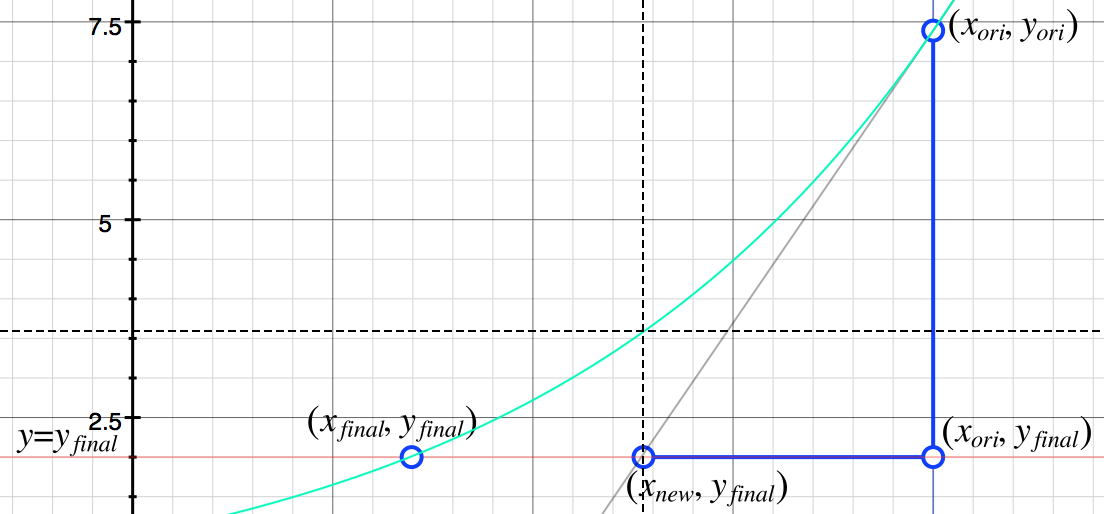
\includegraphics[scale=0.5]{./images/牛顿方法示例图片}
		\caption{牛顿方法示例图}
	\end{figure}

	\item 在逻辑回归中使用牛顿方法的过程
	\begin{enumerate}
		\item 由上图可知,$\tan\alpha = \frac{y_{ori}-y_{final}}{x_{ori}-x_{new}} = \frac{f(x_{ori})-f(x_{final})}{x_{ori}-x_{new}} = f'(x_{ori})$\footnote{$\alpha$是切线$y=f'(x_{ori})x + b$与水平线$y=y_{final}$的夹角,不好标就没画出来了},可以得到
		\begin{equation}
			x_{new} := x_{ori} - \frac{f(x_{ori})-f(x_{final})}{f'(x_{ori})}
		\end{equation}
		
		\item 此时,我们得到了一个新的点$(x_{new}, y_{new})$,相比与原来的点$(x_{ori},y_{ori})$,这个点离最终的$(x_{final}, y_{final})$更近了。

		\item 特殊地,在逻辑回归中,我们要得到的是似然函数$l(\theta)$的极值,极值点的导数为$0$。于是,为了在逻辑回归中使用牛顿方法,我们用$l'(\theta)$代替$f(x)$,且$l'(\theta_{final}) = 0$,于是,上式变成
		\begin{align}
			\theta_{new} &:= \theta_{ori} - \frac{l'(\theta_{ori})-l'(\theta_{final})}{l''(\theta_{ori})} \\
			&:=  \theta_{ori} - \frac{l'(\theta_{ori})}{l''(\theta_{ori})}
		\end{align}
		这就是逻辑回归使用牛顿方法时的迭代方式
	\end{enumerate}

	\item 矩阵表达形式 \\
	将上面的式子改写为矩阵表达的形式,如下
	\begin{equation}
		\theta := \theta - H^{-1}\nabla_{\theta}l(\theta)
	\end{equation}
	其中,$H$称为Hessian\footnote{关于Hessian矩阵的介绍请见附录},是一个$n*n$矩阵
	\begin{equation}
		H_{ij} = \frac{\partial^2l(\theta)}{\partial\theta_i\partial\theta_j}
	\end{equation}

	\item 关于牛顿方法的思考
	\begin{enumerate}
		\item 因为不论我们要得到的是最大值还是最小值,其极值点的导数均为$0$,因此,虽然上述逻辑回归中,我们要得到的时似然函数的极大值,但是,若在其他问题中我们要的得到的时极小值,最终的迭代方式还是一样的。
		\item 但是,通过此方法找到的只是极值点(且每次应该只能找到一个解),很可能只是局部最优,如何保证其为全局最优(最大或最小)呢?。{\color{red}{此项待研究。。}}
	\end{enumerate}

	\item 牛顿方法与梯度下降方法的异同
	\begin{enumerate}
		\item 牛顿方法可以在很少的迭代次数就收敛,而梯度下降要收敛需要迭代的次数可能较多
		\item 但是,牛顿方法每次迭代的计算量较大(因为要计算$H^{-1}$),这在特征维度$n$较大时将会耗费较多的性能
		\item 综上,在特征维度$n$不是太大时,使用牛顿方法能够很快就收敛;但是若特征维度$n$很大时,虽然使用牛顿方法需要迭代的次数较少,但是它每次耗费的计算量太大,整个学习的时间不一定能够比梯度下降少。
	\end{enumerate}
\end{enumerate}















			
		\section{广义线性模型}
\subsection{指数分布族}
\begin{enumerate}
	\item 指数分布族的一般形式
	\begin{equation}
		p(y;\eta) = b(y)e^{\eta^T T(y) - a(\eta)}
	\end{equation}
	其中,$\eta$称为自然参数(Natural Parameter); \\
	$T(y)$为$\eta$\footnote{\color{red}{应该是$\eta$,因为指数分布族的参数只有$\eta$,但正确与否待确认}}的充分统计量(Sufficient Statistic),大部分情况下,$T(y) = y$;在$T(y)=y$时,$\eta$往往为标量; \\
	$a(\eta)$称为 log partition function;
	\item 
\end{enumerate}

\subsection{伯努利分布与高斯分布中,GLM各部分的值}
主要是将伯努利分布(即$0-1$分布)与高斯分布的式子尽可能地转化成指数分布族的一般形式,然后在根据该一般形式写出$\eta$,$T(y)$,$a(\eta)$的形式。\\
\begin{enumerate}
	\item 伯努利分布
	\begin{align}
		P(y;\phi) &= \phi^y(1-\phi)^{1-y} \\
		&= e^{y\ln \phi + (1-y)\ln(1-\phi)} \\
		&= e^{ln{\frac{\phi}{1-\phi}} \cdot y + \ln(1-\phi)}
	\end{align}
	与广义线性模型的一般形式比较,可以发现:
	\begin{align}
		b(y) &= 1 \\
		\eta^T &= \ln{\frac{\phi}{1-\phi}} = \eta \rightarrow \phi = \frac{e^{\eta}}{1+e^{\eta}} \\
		T(y) &= y \\
		a(\eta) &= -\ln(1-\phi) = -\ln{(1-\frac{e^{\eta}}{1+e^{\eta}})} = -\ln{\frac{1}{1+e^\eta}} \\
		&= \ln(1+e^\eta)
	\end{align}

	\item 高斯分布 \\
	在证明使用最小二乘法作为线性回归的Cost Fuction\footnote{最大化$\theta$等同于最大化$\frac{1}{2} \sum_{i=1}^{m}\left(y^{(i)}-\theta^Tx^{(i)}-\mu\right)^2$}的可行性时提到: $J(\theta)$取到最值时的$\theta$值与$\sigma^2$无关(但与$\mu$有关),故在下面的证明中,我们另$\sigma^2=1$,以简化计算
	\begin{align}
		P(y;\mu) &= \frac{1}{\sqrt{2\pi}}e^{-\frac{1}{2}\left(y-\mu\right)^2} \\
		&= \frac{1}{\sqrt{2\pi}} e^{-\frac{y^2-2\mu y +\mu^2}{2}} \\
		&= \frac{1}{\sqrt{2\pi}}e^{-\frac{y^2}{2}} \cdot e^{\mu y-\frac{\mu^2}{2}}
	\end{align}
	故:
	\begin{align}
		b(y) &= \frac{1}{\sqrt{2\pi}}e^{-\frac{y^2}{2}} \\
		\eta^T &= \mu = \eta \\
		T(y) &= y \\
		a(\eta) &= -1\cdot (-\frac{\mu^2}{2}) = \frac{\mu^2}{2} = \frac{\eta^2}{2}
	\end{align}

	\item 注意事项
	\begin{enumerate}
		\item $\eta^T$要在$\eta$为标量时才能直接等于$\eta$,故上面的式子中是在得到$\eta^T$为标量后再写$=\eta$
		\item $a(\eta)$通常不会直接得到关于$\eta$的函数,需要通过$\eta^T$来与$\eta$关联,从而得到$a(\eta)$
	\end{enumerate}
\end{enumerate}

\subsection{如何构造广义线性模型}
\subsubsection{三个假设}
\begin{enumerate}
	\item 假设一:假设$y|x; \theta$服从指数分布族,即$y|x; \theta \sim E(\eta)$
	\item 假设二:假设$h_\theta(x)$ 是$p\left(T(y)|x; \theta\right)$的无偏估计量,即$h_\theta(x)=E\left(T(y)|x; \theta\right)$,并另$T(y)=y$,于是就有
	\begin{equation}
		h(x) = E(y|x)
	\end{equation}
	{\color{red}{暂时对此假设不怎么理解,待后续理解后补充}}
	\item 假设三:假设$\eta = \theta^Tx$ \\
	当$\theta$是一个向量时,$\eta_i = \theta_i^Tx$
	\item 解释说明
	\begin{enumerate}
		\item $y|x; \theta$表示的是一个事件,就像事件$X$,事件$Y$,只是写法比较不一样而已
		\item 在构造广义线性模型中,我们的目的是通过输入的$x$来得到$\theta$,进而得到$y$;因为$T(y)$是$\eta$的充分统计量,因此,我们通过得到$T(y)$的信息来了解$\eta$的信息{\color{red}{(此条正确性待查)}}
	\end{enumerate}
\end{enumerate}

\subsubsection{普通的最小二乘法}
对于普通的最小二乘法,由前面的证明我们知道$\mu = \eta$,故
\begin{equation}\begin{aligned}
	h_\theta(x) &= E(y|x;\theta) \\
	&= \mu \\
	&= \eta \\
	&= \theta^T x
\end{aligned}\end{equation}

\subsubsection{逻辑回归}
对于逻辑回归,由前面的证明可知$\phi=\frac{e^{\eta}}{1+e^{\eta}} = \frac{1}{1+e^{-\eta}}$,故
\begin{equation}\begin{aligned}
	h_\theta(x) &= E(y|x; \theta) \\
	&= \phi \\
	&= \frac{1}{1+e^{-\eta}} \\
	&= \frac{1}{1+e^{-\theta^Tx}}
\end{aligned}\end{equation}


\subsubsection{说明}
\begin{enumerate}
	\item 函数$g(\eta) = E\left[E(T(y);\eta)\right]$将$T(y)$的期望与自然参数$\eta$联系起来
	\item 我们将$g(\eta)$称为正则响应函数(Canonical Response Function)
	\item 将$g(\eta)$的反函数$g^{-1}(y)$称为正则关联函数(Canonical Link Function)
	\item {\color{red}{关于正则响应函数,正则关联函数的理解待补充}}
\end{enumerate}



% 

















			\subsection{Softmax Regression}
\subsubsection{关于$\phi$的说明}
\begin{enumerate}
	\item 对于总共有$k$类的分类问题,因为每个分类出现的概率和为1,故仅有$k-1$维特征是相互独立的
	\item 我们将$p(y=i;\phi)$记为$\phi_i$;于是$\phi_k=p(y=k;\phi)=1-\sum_{i=1}^{k-1}\phi_i$。
\end{enumerate}

\subsubsection{关于$T(y)$的表示法说明}
\begin{enumerate}
	\item 为了描述$T(y)$属于多分类问题中的那一类,我们用$k-1$维向量来描述$T(y)$,其中,若$T(y)$属于第$i$类,则第$i$维值为1,其余均为0\footnote{此种表示方法称为One-Hot}。示例如下:
	\begin{equation}
		T(2) = \left[\begin{matrix} 0 \\ 1 \\ 0 \\ \vdots \\ 0 \end{matrix}\right], \quad
		T(1) = \left[\begin{matrix} 1 \\ 0 \\ 0 \\ \vdots \\ 0 \end{matrix}\right], \quad 
		T(k-1) = \left[\begin{matrix} 0 \\ 0 \\ 0 \\ \vdots \\ 1 \end{matrix}\right]
	\end{equation}
	于是,$T(k)$就是个$\vec{0}$向量\footnote{因为它$0\to n-1$维均不是}
	\begin{equation}
		T(k) = \left[\begin{matrix} 0 \\ 0 \\ 0 \\ \vdots \\ 0 \end{matrix}\right]
	\end{equation}
	\item 为了描述方便,我们使用以下新的表示方法
	\begin{enumerate}
		\item $1\{\cdot\}$,在$\cdot$的值为$True$时,$1\{True\}=1$,否则$1\{False\}=0$。如$1\{2=3\}=0$,$1\{2=2\}=1$
		\item 在以上表示法下,$T(y)$可表示成以下形式
		\begin{align}
			\left(T(y)\right)_i &= 1\{y=i\} \\
			& \downarrow \\
			E\left[\left(T(y)\right)_i\right] &= P(y=i)=\phi_i
		\end{align}
	\end{enumerate}
\end{enumerate}

\subsubsection{证明多项式分布属于指数族分布}
\begin{enumerate}
	\item 在多分类问题中,$p(y;\phi)$表示的含义及其表示方式
	\begin{enumerate}
		\item 与逻辑回归时的二分类一样,$p(y=k;\phi)$表示的是取到第$k$类的概率,用$p(y;\phi)$将$p(y=1;\phi), p(y=2;\phi), \dots, p(y=k;\phi)$表示成一个表达式
		\item 参考逻辑回归的方式,我们将$p(y;\phi)$表示为
		\begin{align}
			p(y;\phi) &= \phi_{1}^{1\{y=1\}}\phi_{2}^{1\{y=2\}}\dots\phi_{k}^{1\{y=k\}} \\
			&= \phi_{1}^{1\{y=1\}}\phi_{2}^{1\{y=2\}}\dots\phi_{k}^{1-\sum_{i=1}^{k-1}1\{y=i\}} \\
			&= \phi_{1}^{\left(T(y)\right)_1}\phi_{2}^{\left(T(y)\right)_2}\dots\phi_{k}^{1-\sum_{i=1}^{k-1}\left(T(y)\right)_i} \\
			&= e^{\left(T(y)\right)_1\ln\phi_1 + \left(T(y)\right)_2\ln\phi_2 + \dots + \left(T(y)\right)_{k-1}\ln\phi_{k-1} + \left[1-\sum_{i=1}^{k-1}\left(T(y)\right)_i\right]\ln\phi_k } \\
			&= e^{\left(T(y)\right)_1\ln\frac{\phi_1}{\phi_k} + \left(T(y)\right)_2\ln\frac{\phi_2}{\phi_k} + \dots + \left(T(y)\right)_{k-1}\ln\frac{\phi_{k-1}}{\phi_k} + \ln\phi_k} \\
			&= b(y)e^{\eta^T T(y) - a(\eta)}
		\end{align}
		\end{enumerate}
	\item 从上式可得
	\begin{align}
		b(y) &= 1 \\
		\eta^TT(y) &= \left(T(y)\right)_1\ln\frac{\phi_1}{\phi_k} + \left(T(y)\right)_2\ln\frac{\phi_2}{\phi_k} + \dots + \left(T(y)\right)_{k-1}\ln\frac{\phi_{k-1}}{\phi_k} \\
		&\downarrow \\
		\eta^T &= \left[\begin{matrix}
		\ln\frac{\phi_1}{\phi_k} \\ \ln\frac{\phi_2}{\phi_k} \\ \vdots \\ \ln\frac{\phi_{k-1}}{\phi_k}
		\end{matrix}\right] \\
		a(\eta) &= -\ln\phi_k
	\end{align}
\end{enumerate}


\subsubsection{使用Softmax进行分类}
\begin{enumerate}
	\item 对于$\eta$中的某一项
	\begin{align}
		\eta_i &= \ln{\frac{\phi_i}{\phi_k}} \\
		&\downarrow \\
		e^{\eta_i} &= \phi_i \\
		&\downarrow \\
		\phi_k e^{\eta_i} &= \phi_i \\
		\phi_k\sum_{i=1}^{k}e^{\eta_i} &= \sum_{i=1}^{k}\phi_i = 1 \\
		&\Downarrow \\
		\phi_i &= \phi_k\cdot e^{\eta_i} \\
		&= e^{\eta_i} \cdot \frac{1}{\sum_{j=1}^{k}e^{\eta_j}}
	\end{align}
	如上所示,$\phi_i = \frac{e^{\eta_i}}{\sum_{j=1}^{k}e^{\eta_j}}$称为Softmax函数
	\item 最后,再使用前面的假设三:$\eta_i = \theta_i^Tx, \quad i=1,2, \dots, k-1, \quad \theta_i \in {\rm I\!R}^{n+1}$,可得到
	\begin{align}
		p(y=i|x; \theta) &= \phi_i \\
		&= \frac{e^{\eta_i}}{\sum_{j=1}^{k}e^{\eta_j}} \\ 
		&= \frac{e^{\theta_i^Tx}}{\sum_{j=1}^{k}e^{\theta_j^Tx}}
	\end{align}
	\item 故
	\begin{align}
		h_\theta(x) &= E\left[T(y)|x;\theta\right] \\
		&= E\left[\left[\begin{matrix} 1\{y=1\} \\ 1\{y=2\} \\ \vdots \\ 1\{y=k-1\} \end{matrix}\right|x;\theta\right] \\
		&= \left[\begin{matrix}\phi_1 \\ \phi_2 \\ \vdots \\ \phi_{k-1} \end{matrix}\right] \\ 
		&= \left[\begin{matrix}
		\frac{e^{\theta_1^Tx}}{\sum_{j=1}^{k}e^{\theta_j^Tx}} \\
		\frac{e^{\theta_2^Tx}}{\sum_{j=1}^{k}e^{\theta_j^Tx}} \\
		\vdots \\
		\frac{e^{\theta_{k-1}^Tx}}{\sum_{j=1}^{k}e^{\theta_j^Tx}}
		\end{matrix}\right]
	\end{align}
	如上,最终$h_\theta(x)$可得到$k-1$维向量,通过总概率为1得到第$k$维的概率值,由此可以得到每一种类别的概率值
	\item 以上得到多分类中每种分类概率值的方法就叫做Softmax回归(Softmax Regression)
\end{enumerate}


\subsubsection{参数$\theta$的拟合方式}
使用对数似然估计方法
\begin{align}
	l(\theta) &= \sum_{i=1}^{m}\ln p\left[y^{(i)}|x^{(i)};\theta\right] \\
	&= \sum_{i=1}^{m} \ln \prod_{l=1}^{k}\left[
	\frac{e^{\theta_l^Tx^{(i)}}}{\sum_{j=1}^{k}e^{\theta_l^Tx^{(i)}}}
	\right]^{1\{y^{(i)}=l\}}
\end{align}
{\color{red}{后续待补充}}













		\section{生成学习算法}
\subsection{生成学习算法简介}

\subsubsection{判别学习算法\&生成学习算法}
\begin{enumerate}
	\item 判别学习算法:计算$p(y|x)$,例如逻辑回归中计算$p(y=1|x)$与$p(y=0|x)$
	\item 生成学习算法:计算$p(x|y)$与$p(y)$,然后通过贝叶斯公式$p(y|x) = \frac{p(x|y)p(y)}{p(x)}$计算得到$p(y|x)$
	\begin{enumerate}
		\item 不论$p(y|x)$中$y$的值为多少,式中的$p(x)$均是一样的值(可通过全概率公式计算得到),因此,对于$p(y|x)$较大的$y=k$,$p(x|y)p(y)$也较大,因此,在最优化过程中,可以不计算$p(x)$,于是优化过程变为
		\begin{align}
			arg\max{p(y|x)} &= arg \max_y{\frac{p(x|y)p(y)}{p(x)}} \\
			&= arg\max_y{p(x|y)p(y)}
		\end{align}
		省去了计算$p(x)$的过程
	\end{enumerate}
	
	\item 判别学习算法是给出一系列特征,得到这些特征应该是哪一种结果;生成学习算法学习的是某一种结果应该有什么特征。

\end{enumerate}




















			\subsection{高斯判别分析}
以下内容中均假设$p(x|y)$服从多重正态分布(高斯分布)

\subsubsection{多重正态分布简介}
\begin{enumerate}
	\item $n$重正态分布可由均值向量$\mu \in {\rm I\!R}^n$和协方差矩阵$\Sigma \in {\rm I\!R}^{n\times n}$确定,记做$N(\mu, \Sigma)$,表示为:
	\begin{equation}
		p(x; \mu, \Sigma) = \frac{1}{(2\pi)^{\frac{n}{2}}|\Sigma|^\frac{1}{2}}e^{-\frac{1}{2}(x-\mu)^T\Sigma^{-1}(x-\mu)}
	\end{equation}
	其中,$|\Sigma|$是协方差矩阵$\Sigma$的行列式;$\Sigma=\mathrm{Cov}(X) = E(XX^T) - E(X)\left[E(X)\right]^T$,$X$的期望为$E(X) = \int_{x}xp(x;\mu,\Sigma)dx = \mu$
\end{enumerate}

\subsubsection{高斯判别分析模型}
\begin{enumerate}
	\item 高斯判别分析模型针对的是连续型随机变量,如果是离散型随机变量可使用后续会讲到的朴素贝叶斯
	\item 我们假设$p(x|y)$服从多重高斯分布,于是
	\begin{align}
		y & \sim B(1, \phi) = Bernoulli(\phi) \\
		x|y=0 &\sim N(\mu_0, \Sigma) \\
		x|y=1 &\sim N(\mu_1, \Sigma)
	\end{align}
	于是,其概率密度为:
	\begin{align}
		p(y) &= \phi^y(1-\phi)^{1-y} \\
		p(x|y=0) &= \frac{1}{(2\pi)^{\frac{n}{2}}|\Sigma|^\frac{1}{2}}e^{-\frac{1}{2}(x-\mu_0)^T\Sigma^{-1}(x-\mu_0)} \\
		p(x|y=1) &= \frac{1}{(2\pi)^{\frac{n}{2}}|\Sigma|^\frac{1}{2}}e^{-\frac{1}{2}(x-\mu_1)^T\Sigma^{-1}(x-\mu_1)}
	\end{align}
	在上式中,$\phi, \mu_0, \mu_1, \Sigma$就是我们要求的参数(注意,有2个$\mu$
	,共享1个$\Sigma$)。
	\begin{enumerate}
		\item $p(y)$表示的$y=k, k=0,1$的可能性
		\item $p(x|y=k)$表示的是,在已知$y=k$的情况下, $x$长这个样子的可能性
	\end{enumerate}
	\item 其对数似然函数为:
	\begin{align}
		l(\phi, \mu_0, \mu_1, \Sigma) &= \log \prod_{i=1}^{m} p\left(x^{(i)}, y^{(i)}; \phi, \mu_0, \mu_1, \Sigma\right) \\
		&= \log \prod_{i=1}^{m} p\left(x^{(i)}|y^{(i)}; \mu_0, \mu_1, \Sigma\right)p\left(y^{(i)};\phi\right)
	\end{align}
	注意$p(x|y)$中并没有参数$\phi$,$p(y)$中只有参数$\phi$\footnote{若对此有疑问,可回去复习一下似然函数}。
	\item 求解似然函数后可得参数如下
	\begin{align}
		\phi &= \frac{1}{m} \sum_{i=1}^{m}1\{y^{(i)=1}\} \\
		\mu_0 &= \frac{\sum_{i=1}^{m}1\{y^{(i)}=0\}x^{(i)}}{\sum_{i=1}^{m}1\{y^{(i)}=0\}} \\
		\mu_1 &= \frac{\sum_{i=1}^{m}1\{y^{(i)}=1\}x^{(i)}}{\sum_{i=1}^{m}1\{y^{(i)}=1\}} \\
		\Sigma &= \frac{1}{m}\sum_{i=1}^{m}\left(x^{(i)}-\mu_{y^{(i)}}\right)\left(x^{(i)}-\mu_{y^{(i)}}\right)^T
	\end{align}
	下面解释下以上各参数表达式的意义: \\
	$\phi$:表示所有数据中$y=1$所占的比例; \\
	$\mu_0$: 其分母表示所有数据中$y=0$的数目,分子表示$y=0$对应的$x$的和,表示的就是$y=0$所对应的$x$的均值;$\mu_1$同理 \\
	$\Sigma$: 协方差矩阵,前面已说过,不再赘述
	\item 说明
	\begin{enumerate}
		\item 使用通过高斯判别分析得到的模型得到的是两个高斯分布
		\item 这两个高斯分布有共同的协方差$\Sigma$,但是其期望$\mu$不一样,若画出其等高线,在图形上表现为两个等高线形状(由$\Sigma$决定)一样,但是其中心(由$\mu$决定)不一样。
	\end{enumerate}
\end{enumerate}

\subsubsection{高斯判别分析\&逻辑回归}
\begin{enumerate}
	\item 如果我们将$\phi, \mu_0, \mu_1, \Sigma$看出$x$的函数,进行整理后最终可得到
	\begin{equation}
		p(y=1|x; \phi, \mu_0, \mu_1, \Sigma) = \frac{1}{1+e^{-\theta^Tx}}
	\end{equation}
	其中,$\theta$是$\phi, \mu_0, \mu_1, \Sigma$的函数
	\item 在我们的证明过程中,我们假设了$p(x|y)$服从高斯分布,相较于逻辑回归,GDA做了更强的假设。
	\item 如果$p(x|y)$服从多重高斯分布,则$p(y|x)$服从逻辑回归;但是,从$p(y|x)$服从逻辑回归无法得到$p(x|y)$服从多重高斯分布。这说明GDA需要更多的条件,其做了更强的假设。
	\item 在两种算法的准确性上:如果$p(x|y)$确实服从或近似服从高斯分布(即我们对其做的假设正确),那么GDA能够更好地进行预测;但是,若我们的假设错误(即$p(x|y)$实际并不服从或近似服从高斯分布,可能是泊松分布或其他),此时,逻辑回归能得到更好的效果
	\item 在数据集$m$很大时,GDA可以得到比大部分算法更好的结果(包括逻辑回归);甚至在数据集较小时,GDA也往往比逻辑回归好
	\item 通常来讲,使用生成学习算法需要的数据更少(因为做了高斯分布的假设,从高斯分布继承了很多性质),因为大部分情况下,我们的数据虽然不是精确的高斯分布,但近似服从高斯分布。
	\item 因为逻辑回归的假设更弱(可理解为需要的条件更少),因此其具有更好的鲁棒性(可理解为适应能力更好),即使$p(y|x)$并不符合也不近似符合高斯分布,逻辑回归也能较好地预测。
	\item 使用逻辑回归可能需要比较多的数据样本
\end{enumerate}
















			\subsection{朴素贝叶斯}
\begin{enumerate}
	\item 在GDA中,随机变量$X$是连续的,当随机变量是离散值时,我们使用朴素贝叶斯来进行预测
	\item 朴素贝叶斯举例介绍:以通过邮箱中的文本预测是否为垃圾邮件为例,$y=1$表示该邮件是垃圾邮件
	\begin{enumerate}
		\item 对每封邮件建立词向量\footnote{此处的词向量比较简单,与文本分析(NLP)中的词向量不一样,也不是One-Hot的形式},每个词在向量中占据一个位置,若该词存在,则将该位的值设为1,若不存在则设为0,得到如下向量
		\begin{align}
			x = \left[\begin{matrix}1 \\ 0 \\ 0 \\ \vdots \\ 1 \\ \vdots \\ 0 \end{matrix}\right] \quad
			\begin{matrix}a \\ ad \\ address \\ \vdots \\ buy \\ \vdots \\ zygmurgy \end{matrix}
		\end{align}
		如上所示,该邮件中有a, buy等,没有ad, address, zygmurgy等。
		\footnote{一般来说,建议通过扫描训练集来获取可能出现的词(而不是从字典中获取),这样做一方面可以减小建模时的特征数,节省计算量和存储空间;另一方面还可以避免出现一些字典中没有的词(如CS299,或一些人名等)\\
		另外,还可以将一些无实意、出现频率又比较高的词去除,如a, an, the等}
		\item 若要使用多项式分布来进行预测,按照之前的逻辑回归方式,在词向量维度较多时并不可取(PS:讲义中的$2^{50000}-1$看起来似乎有问题,对$50000$个词建模只需要有$50000+1$个参数,哪来的$2^{50000}-1$??{\color{red}{待研究...}})
		\item 为了更方便地进行建模,我们做了一个假设:假设对于给定的$y$,$x_i$($x_i$指词向量中的第$i$个词)是相互条件独立的,即$p(x_2|y, x_1) = p(x_2|y)$,给定的$x_1$条件并不影响$p(x_2|y)$。此假设称为{\color{blue}{朴素贝叶斯假设}}。由此得到的分类器称为{\color{blue}{朴素贝叶斯分类器}}。
		\item 根据以上假设,我们可以得到以下式子:
		\begin{align}
			p(x_1, \dots, x_n|y) &= p(x_1|y)p(x_2|y, x_1)p(x_3|y, x_1, x_2)\dots p(x_n|y, x_1, x_2, \dots, x_{n-1}) \\
			&= p(x_1|y)p(x_2|y)p(x_3|y)\dots p(x_n|y) \\
			&= \prod_{i=1}^{n}p(x_i|y)
		\end{align}
		\item 与GDA类似,上式由参数$\phi_{i|y=1}=p(x_i=1|y=1)$,$\phi_{i|y=0}=p(x_i=1|y=0)$,$\phi_y=p(y=1)$决定。似然函数可表示为:
		\begin{align}
			L(\phi_y, \phi_{i|y=0}, \phi_{i|y=1}) = \prod_{i=1}^{n}p(x^{(i)}|y^{(i)})
		\end{align}
		\item 通过最大似然估计,可得
		\begin{align}
			\phi_{j|y=1} &= \frac{\sum_{i=1}^{m}1\{x_j^{(i)}=1 \cap y^{(i)}=1\}}{\sum_{i=1}^{m}1\{y^{(i)}=1\}} \\
			\phi_{j|y=0} &= \frac{\sum_{i=1}^{m}1\{x_j^{(i)}=1 \cap y^{(i)}=0\}}{\sum_{i=1}^{m}1\{y^{(i)}=0\}} \\
			\phi_y &= \frac{\sum_{i=1}^{m}1\{y^{(i)}=1\}}{m}
		\end{align}
		其中: \\
		$\cap$表并集,即两个条件同时满足 \\
		$\phi_{j|y=1}$表示出现词$x_j$的垃圾邮件在所有垃圾邮件中所占的比例 \\
		$\phi_{j|y=0}$表示出现词$x_j$的非垃圾邮件在所有非垃圾邮件中所占的比例 \\
		$\phi_y$表示垃圾邮件占所有邮件的比例
		\item 使用贝叶斯公式计算$p(y|x)$
		\begin{align}
			p(y=1|x) &= \frac{p(x|y=1)p(y=1)}{p(x)} \\
			&= \frac{\prod_{i=1}^{n}p(x_i|y=1)p(y=1)}{\left[\prod_{i=1}^{n}p(x_i|y=1)\right]p(y=1)+\left[\prod_{i=1}^{n}p(x_i|y=0)\right]p(y=0)}
		\end{align}
		对$p(y=0|x)$同理,通过比较那个概率更高\footnote{所以,其实$p(x)$并没有必要求,虽然也不难求}来判断是否为垃圾邮件。
		\item 虽然以上过程中只是二分类,但实际上,对于多分类也是以上的套路;
		\item 对于连续型随机变量,也可以对其分段离散化,然后使用朴素贝叶斯进行预测
	\end{enumerate}
\end{enumerate}

\subsection{拉普拉斯平滑}
\subsubsection{背景介绍}
\begin{enumerate}
	\item 在朴素贝叶斯中,若在预测时出现了一个我们训练集中没有的词,那么预测结果为
	\begin{align}
		\phi_{{x_j}|y=1} &= \frac{\sum_{i=1}^{m}1\{x_j^{(i)}=1 \cap y^{(i)}=1\}}{\sum_{i=1}^{m}1\{y^{(i)}=1\}} \\
		&= 0 \\
		\phi_{{x_j}|y=1} &= \frac{\sum_{i=1}^{m}1\{x_j^{(i)}=1 \cap y^{(i)}=0\}}{\sum_{i=1}^{m}1\{y^{(i)}=0\}} \\
		&= 0 \\
		p(y=1|x) &= \frac{\prod_{i=1}^{n}p(x_i|y=1)p(y=1)}{\left[\prod_{i=1}^{n}p(x_i|y=1)\right]p(y=1)+\left[\prod_{i=1}^{n}p(x_i|y=0)\right]p(y=0)} \\
		&= \frac{0}{0}
	\end{align}
	此时出现了$\frac{0}{0}$的情况,没法进行预测。为了解决此问题,我们可以使用拉普拉斯平滑。\footnote{吴恩达的视频中,举了一个已知前面5次比赛都失败,预测第6次失败的概率,可以看下。}
\end{enumerate}

\subsubsection{拉普拉斯平滑介绍}
\begin{enumerate}
	\item $\frac{0}{0}$出现的原因 \\
	由前面$\phi_j = \frac{\sum_{i=1}^{m}1\{z^{(i)}=j\}}{m}$可知,$\phi_j$为出现$z^{(i)}=j$的数据占总数据的比例,在$z^{(i)}=j$在训练集中未出现过时,就会出现$\phi_j=0$\footnote{在$=0$处频数为0,在$=1$处频数也为0},从而导致出现$\frac{0}{0}$的情况,为了解决此问题,我们队$\phi_j$稍作更改:
	\begin{equation}
		\phi_j = \frac{\sum_{i=1}^{m}1\{z^{(i)}=j\}+1}{m+k}
	\end{equation}
	经过此方式处理后:
	\begin{enumerate}
		\item $\sum_{j=1}^{k}\phi_j = 1$仍旧成立
		\item 对任意$\phi_j \neq 0$
	\end{enumerate}
\end{enumerate}














			\subsection{文本分类}
\begin{align}
	\phi_{k|y=1} &= \frac{\sum_{i=1}^{m}\sum_{j=1}^{n}1\{x_j^{(i)}=k \cap y^{(i)}=1\}+1}{\sum_{i=1}^{m}1\{y^{(i)}=1\}n_i + |V|} \\
	\phi_{k|y=0} &= \frac{\sum_{i=1}^{m}\sum_{j=1}^{n}1\{x_j^{(i)}=k \cap y^{(i)}=0\}+1}{\sum_{i=1}^{m}1\{y^{(i)}=0\}n_i + |V|}
\end{align}


详情略, 待补充









		\section{支持向量机}

\subsection{逻辑回归的缺陷}
\begin{enumerate}
	\item 按照逻辑回归的计算方式,我们得到的是一个分隔线(或平面或超平面\footnote{1维称为线,2维称为平面,更多维就称为超平面}),对于我们的数据点,总有一些点离超平面较近(如点C),有一些点离超平面较远(如点A);对于离超平面较远的点,我们有很大把握保证我们的预测是准确的,但是,对于离超平面较近的点我们就没把握了。
	\begin{figure}[htbp]
		\centering
		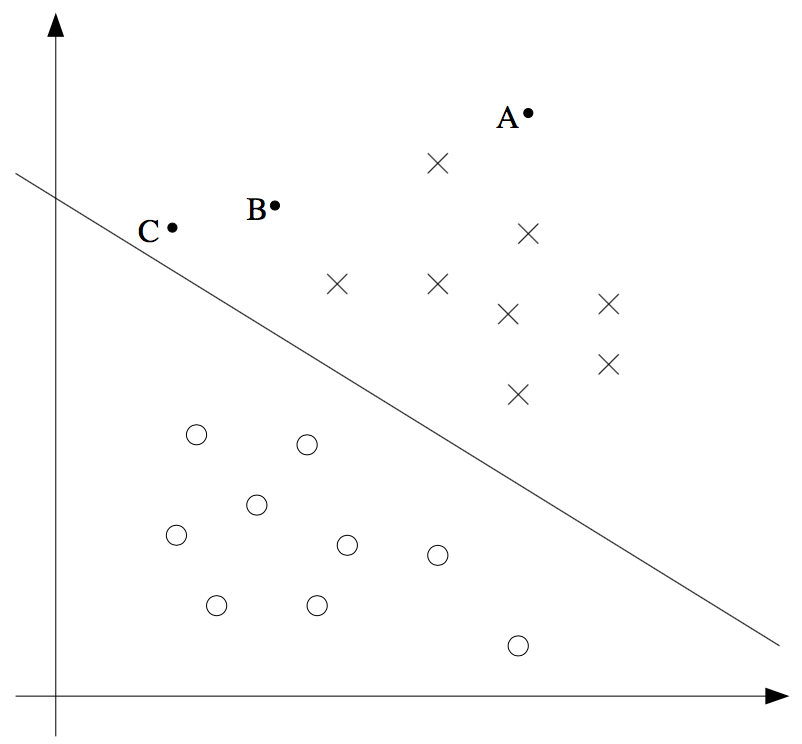
\includegraphics[scale=0.5]{images/逻辑回归缺陷讲述}
		\caption{支持向量机实例用图}
	\end{figure}
\end{enumerate}

\subsection{SVM前言}
\begin{enumerate}
	\item 在后续介绍SVM过程中,为了描述方便,我们对之前逻辑回归的一些描述做了更改
	\item 将$h_\theta(x)$更改为$h_{w,b}(x)$,其中:$w \to \left[\begin{matrix}\theta_1 \\ \theta_2 \\ \vdots \\ \theta_n  \end{matrix}\right]$,$b \to \theta_0$\footnote{此处为了表达方便,使用$\to$来表达类似的对应关系,且勿将其当做等于"$=$"}
	\begin{align}
		h_{w,b}(x) = g(w^Tx+b)
	\end{align}
	\item 将类标签$y$改为$\{-1, 1\}$;将$h=g(w^T+b)$的值从值域$\{0,1\}$切换到$\{-1, 1\}$,其中,$0\to -1$,$1\to 1$
	,且取消原有的$x_0=1$假设。通过此方式将$h(x)$由参数$\theta$变成了参数$(w, b)$,将截距项$b$与其他项分隔开,以便分析
\end{enumerate}

\subsection{Margin介绍}
\subsubsection{函数间隔}
\begin{enumerate}
	\item 对于数据点$(x^{(i)}, y^{(i)})$,其函数间隔定义为:
	\begin{align}
		\hat{\gamma}^{(i)} = y^{(i)}(w^Tx^{(i)} + b)
	\end{align}
	\item 对于$y^{(i)}=1$的点,为了让函数间隔$\hat{\gamma}$越大,我们需要让$w^Tx^{(i)} + b$正向越大;
	\item 对于$y^{(i)}=-1$的点,为了让函数间隔$\hat{\gamma}$越大,我们需要让$w^Tx^{(i)} + b$负向越大;
	\item 对于给定的训练集$S=\{(x^{(i)}, y^{(i)}); \quad i = 1, \dots, m\}$,我们将其中最小的函数间隔记为$\hat{\gamma}$:
	\begin{align}
		\hat{\gamma} = \min_{i=1,\dots,m}\hat{\gamma}^{(i)}
	\end{align}
	\item 对于函数间隔,若将参数$(w,b)$扩大2倍2为$(2w,2b)$,函数间隔的值$\hat{h}_{w,b}(x)$也变成了原来的2倍,但实际上,这对训练的效果并没有影响,原来错误的现在还是错误
\end{enumerate}

\subsubsection{几何间隔}
\begin{enumerate}
	\item 几何间隔表示为$\gamma^{(i)}$\footnote{与函数间隔相比,少了头顶的帽子: $\hat{ }$}。
	\item 对于数据点$(x^{(i)}, y^{(i)})$,其几何间隔定义为\footnote{证明过程:使用向量的加法表示出超平面外的某点的向量表示形式,然后两边乘以$w^T$,整理一下就能得到几何间隔表示形式,详情略}:
	\begin{align}
		\gamma^{(i)} &= \frac{\hat{\gamma}^{(i)}}{\|w\|}  \\
		&= \frac{y^{(i)}(w^Tx^{(i)} + b)}{\|w\|}  \\
		&=  y^{(i)} \left(\left(\frac{w}{\|w\|}\right)^T x^{(i)} + \frac{b}{\|w\|}\right)
	\end{align}
	\footnote{$\|w\|$是矩阵的范数,$\|w\|^2=w^Tw$}
	\item 当$\|w\|=1$时,几何间隔与函数间隔相等
	\item 相较于函数间隔,几何间隔任意缩放参数$(w,b)$不影响$h_{w,b}(x)$的值;鉴于此性质,我们可以在训练时对$w, b$视需求进行缩放
	\item 同样,对于给定的训练集$S=\{(x^{(i)}, y^{(i)}); \quad i = 1, \dots, m\}$,我们将其中最小的几何间隔记为$\gamma$:
	\begin{align}
		\gamma = \min_{i=1,\dots,m}\gamma^{(i)}
	\end{align}
\end{enumerate}

\subsubsection{函数间隔\&几何间隔}
\begin{enumerate}
	\item 当预测正确时,二者都是正值;当预测错误是,二者都是负值。
\end{enumerate}

\subsubsection{对SVM设计函数间隔、几何间隔原因的思考}
{\color{red}{注意,此部分内容仅仅是我自己的理解,不见得正确,请批判性地看。}}
\begin{enumerate}
	\item 与之前的逻辑回归类似,此处$w^Tx+b=0$是用来判断预测值$h_{w,b}(x)$取1或-1的分界线:若$w^Tx+b\geq0$,则通过激活函数$g(z)$让$h_{w,b}(x)=g(w^Tx+b)=1$,反之,让$h_{w,b}(x)=-1$。$w^Tx+b=0$相当于门槛的角色,没过门槛是一个世界,过了门槛又是另一个世界
	% \item 与前面逻辑回归一样,$w^Tx+b$与$\theta^Tx$计算出来的结果意义一样,且都是通过激活函数$g(z)$(虽然两者的$g(z)$形式不一样)来得到预测值;
	\item 但是,两者的激活函数$g(z)$不一样,其得到的结果也不一样,逻辑回归的$g(z)$得到的是概率值,后续也是通过让概率值达到最大来优化算法;
	\item SVM的$g(z)$得到的结果是一个我也不知道代表什么意义的值,后续优化的对象是预测值与门槛$w^Tx+b=0$的几何间隔
	\item 但是SVM优化的几何间隔又与线性回归中使用点与点间的距离$h_\theta(x^{(i)})-y^{(i)}$不大一样:它除了与线性回归类似计算了与{\color{red}{门槛}}的距离$w^Tx^{(i)}-b-0$\footnote{此处计算的是与{\color{red}{门槛}}的距离,对于门槛,$w^Tx-b$的值为0}之外,还乘以了它的实际值$y^{(i)}$,$y^{(i)}$的出现可以纠正它的正负号,若预测正确(即预测值与实际值在门槛的同一边),则得到的结果为正值;否则为负值,将此定义为函数间隔;又因为让函数间隔最大化不一定能够得到最优的门槛(总有些投机倒把的通过增大$w,b$来达到目的),于是我们又对函数间隔除以$\|w\|$,解决了这个Bug,将此定义为几何间隔。于是对SVM的优化就是对几何间隔最大值的优化\footnote{为什么对线性回归的优化是取最小值,而对SVM的优化是取最大值?这就是我们要能理解每一步推理目的的原因了}。
\end{enumerate}





















			\subsection{最优间隔分类器-优化目标}
\subsubsection{将难以优化的目标转为容易优化的}
\begin{enumerate}
	\item 通过前面的讲述我们知道,为了对给定的数据集进行分类,我们需要找到使得几何间隔最大化的决策边界(在下面的讲述中,先假设我们会遇到的数据集都是线性可切分的,等我们讲到核函数时再去除这个假设)。于是,可以用以下的式子来描述我们要优化的目标
	\begin{align}
		\max_{\gamma, w, b} \gamma
	\end{align}
	根据前面的定义:$\gamma = \min_{i=1,\dots,m}\gamma^{(i)}$,$\gamma$是所有数据点中几何间隔最小值,所以,对于任意数据点,其几何间隔均应大于$\gamma$\footnote{这是约束条件,请注意优化目标与约束条件的差别。}:
	\begin{align}
		y^{(i)}\frac{(w^Tx^{(i)}+b)}{\|w\|} \geq \gamma, \quad i=1, 2, \dots, m
	\end{align}
	因为对于几何间隔,缩放$w$或$b$或都缩放不会影响决策边界的位置\footnote{决策边界始终由$w^Tx^{(i)}+b=0$确定},于是,我们定义$\|w\|=1$,让几何间隔与函数间隔相等,于是:
	\begin{align}
		&\text{优化目标:} \\
		& \qquad \max_{\gamma, w, b} \gamma \\
		&\text{约束条件:} \\
		& \qquad y^{(i)}(w^Tx^{(i)}+b) \geq \gamma, \quad i=1, 2, \dots, m \\
		& \qquad \|w\| = 1
	\end{align}

	\item 经过上面的转化后,$\|w\|=1$这个约束还是不好处理,我们需要想办法去除这个约束,于是将优化目标$\gamma$改写为$\frac{\hat{\gamma}}{\|w\|}$\footnote{课上有人问为什么要使用函数间隔?为什么要对它除以$\|w\|$?实际上$\frac{\hat{\gamma}}{\|w\|}$只是$\gamma$的另一种表述,为了后续消去不好处理的约束$\|w\| = 1$才这样处理的。}:
	\begin{align}
		\max_{\gamma, w, b} \frac{\hat{\gamma}}{\|w\|}
	\end{align}
	约束条件变为:
	\begin{align}
		y^{(i)}\frac{(w^Tx^{(i)}+b)}{\|w\|} \geq \frac{\hat{\gamma}}{\|w\|}, \quad i=1, 2, \dots, m
	\end{align}
	消去$\|w\|$,得:
	\begin{align}
		&\text{优化目标:} \\
		& \qquad \max_{\gamma, w, b} \frac{\hat{\gamma}}{\|w\|} \\
		&\text{约束条件:} \\
		& \qquad y^{(i)}(w^Tx^{(i)}+b) \geq \hat{\gamma}, \quad i=1, 2, \dots, m
	\end{align}
	如上,经过这样的转化,我们将$\|w\|$消掉了,同时$\|w\| = 1$的假设也可以取消了。

	\item 我们令$\hat{\gamma}=1$\footnote{这样做是合理的,因为不论$\hat{\gamma}$取何值,我们都可以通过缩放$\|w\|$来消除实际的$\hat{\gamma}$与$\hat{\gamma}=1$的差距}\footnote{有的地方会将两条经过支持向量的直线标记为$w^Tx+b=1$和$w^Tx+b=-1$,这是正确的,因为,函数间隔中,$y^{(i)}$的作用只是改变函数间隔$\hat{\gamma}$的正负号,而支持向量对应的就是函数间隔为1的点,代入后就可以得到这两条直线的方程},于是优化目标变成:
	\begin{align}
		\max_{\gamma, w, b} \frac{1}{\|w\|}
	\end{align}
	最大化$\frac{1}{\|w\|}$也即最小化$\|w\|$,即最小化$\|w\|^2$,故:
	\begin{align}
		&\text{优化目标:} \\
		& \qquad \min_{\gamma, w, b} \frac{1}{2}\|w\|^2 \\
		&\text{约束条件:} \\
		& \qquad y^{(i)}(w^Tx^{(i)}+b) \geq 1, \quad i=1, 2, \dots, m
	\end{align}
\end{enumerate}




































			\subsection{拉格朗日对偶规划}
\subsubsection{拉格朗日乘数法}
\begin{enumerate}
	\item 在等式约束下求最优问题求解中可使用拉格朗日乘数法,其要解决的问题可表述如下:
	\begin{align}
		&\text{优化目标:} \\
		& \qquad \min_{w} f(w) \\
		&\text{约束条件:} \\
		& \qquad h_i(w) = 0, \quad i=1,\dots,l
	\end{align}
	$l$是等式约束的个数
	\item 其拉格朗日函数为:
	\begin{align}
		\mathcal{L}(w,\beta) = f(w) + \sum_{i=1}^{l}\beta_ih_i(w)
	\end{align}
	\item 求拉格朗日函数的偏导数
	\begin{align}
		\frac{\partial \mathcal{L}}{\partial w_i} &= 0\\
		\frac{\partial \mathcal{L}}{\partial \beta_i} &= 0
	\end{align}
	求解上式,得到$w, \beta$即可
\end{enumerate}

\subsubsection{拉格朗日对偶规划}
\begin{enumerate}
	\item 对于有不等约束的问题,拉格朗日乘数法就无能为力了;这时就需要用拉格朗日对偶规划,其所要解决的问题可表述如下:
	\begin{align}
		&\text{优化目标:} \\
		& \qquad \min_{w} f(w) \\
		&\text{约束条件:} \\
		& \qquad g_i(w) \leq 0, \quad i=1,\dots,k \\
		& \qquad h_i(w) = 0, \quad i=1,\dots,l
	\end{align}
	$k, l$为对应约束的个数。\\
	称其为原问题。
	\item 其Generalized Lagrangian\footnote{{\color{red}{不知道怎么翻译}}}为:
	\begin{align}
		\mathcal{L}(w, \alpha, \beta) = f(w) + \sum_{i=1}^{k}\alpha_ig_i(w) + \sum_{i=1}^{l}\beta_ih_i(w)
	\end{align}
	\item 下面我们定义以下式子:
	\begin{align}
		\theta_{\mathcal{P}}(w) = \max_{\alpha, \beta; \alpha_i\geq0} \mathcal{L}(w, \alpha, \beta)
	\end{align}
	注意,在上面的式子中,我们对$\alpha_i$做了限制:$\alpha_i\geq 0$,于是,$\theta_{\mathcal{P}}(w)$便有了以下性质:
	\begin{enumerate}
		\item 当$g_i(w)$不满足约束条件,即$g_i(w)>0$时,为了使$\mathcal{L}(w, \alpha, \beta)$取到更大,我们只需要让$\alpha_i$更大就行,很显然,此时$\max \mathcal{L}(w, \alpha, \beta) = +\infty = \theta_{\mathcal{P}}(w)$
		\item 当$h_i(w)$不满足约束条件时,即$h_i(w)>0$或$h_i(w)<0$,我们同样只需要更改$\beta_i$的值就能让$\max \mathcal{L}(w, \alpha, \beta)$取到$+\infty$
		\item 当$g_i(w)$与$h_i(w)$均满足约束条件时,$\sum_{i=1}^{k}\alpha_i g_i(w)$的最大值是0;$\sum_{i=1}^{l}\beta_ih_i(w)$始终为0;所以,$\theta_{\mathcal{P}}(w)=\max_{\alpha, \beta; \alpha_i\geq0} \mathcal{L}(w, \alpha, \beta)=f(w)$
		\item 综上,我们可以得到以下式子:
		\[ \theta_{\mathcal{P}}(w)=\begin{cases}
		f(w) \quad \text{符合所有约束条件} \\
		+\infty \quad \text{其他}
		\end{cases} \]
	\end{enumerate}

	\item 通过上面的式子我们可以知道,在满足所有约束条件的情况下,$f(w)=\theta_{\mathcal{P}}(w)$,求解$f(w)$的最小值就等同于求解$\theta_{\mathcal{P}}(w)$的最小值(所以我们将$\theta_{\mathcal{P}}(w)$称为{\color{blue}{原问题}}),于是我们的优化目标就变成了:
	\begin{align}
		\min_{w} \max_{\alpha, \beta; \alpha_i \geq 0} \mathcal{L}(w, \alpha, \beta)
	\end{align}
	注意:
	\begin{enumerate}
		\item 对于$\min_{w}$,这是由我们的优化目标$\min_{w}f(w)$带来的
		\item $\max_{\alpha, \beta; \alpha_i \geq 0} \mathcal{L}(w, \alpha, \beta)$是一个整体,此式子表示的是取得$\mathcal{L}(w, \alpha, \beta)$的最大值的最小值
	\end{enumerate}

	\item 相对于前面的求拉格朗日函数最大值$\theta_{\mathcal{P}}(w) = \max_{\alpha, \beta; \alpha_i\geq0} \mathcal{L}(w, \alpha, \beta)$,其{\color{blue}{对偶问题}}\footnote{为什么要讲到其对偶问题呢?后面会讲到。}为求拉格朗日函数的最小值:
	\begin{align}
		\theta_{\mathcal{D}}(\alpha, \beta) = \min_{w} \mathcal{L}(w, \alpha, \beta)
	\end{align}
	对偶问题对应的{\color{blue}{对偶优化问题}}为:
	\begin{align}
		\max_{\alpha, \beta;\alpha_i \geq 0} \theta_{\mathcal{D}}(\alpha, \beta) = \max_{\alpha, \beta;\alpha_i \geq 0} \min_{w} \mathcal{L}(w, \alpha, \beta)
	\end{align}
	\footnote{注意,这个对偶优化问题并不是我们推导出来的,可以说是我们为了后续需要设计出来的,所以不要去想为什么这个式子是这样子的了。}

	\item 对比一下原问题与其对偶问题,可以发现,两者之间的差别只是对调了求最大值$\max_{\alpha, \beta;\alpha_i \geq 0}$与最小值$\min_{w}$的顺序。在后面的描述中,我们用$p^{*}$表示原问题的最优解,用$d^{*}$表示对偶问题的最优解:
	\begin{align}
		p^{*} &= \min_{w} \max_{\alpha, \beta; \alpha_i \geq 0} \mathcal{L}(w, \alpha, \beta) \\
		d^{*} &= \max_{\alpha, \beta;\alpha_i \geq 0} \min_{w} \mathcal{L}(w, \alpha, \beta)
	\end{align}

	\item 原问题与其对偶问题有以下性质:
	\begin{align}
		d^{*} = \max_{\alpha, \beta;\alpha_i \geq 0} \min_{w} \mathcal{L}(w, \alpha, \beta) \leq 
		\min_{w} \max_{\alpha, \beta; \alpha_i \geq 0} \mathcal{L}(w, \alpha, \beta) = p^{*}
	\end{align}
	在一些特定条件(KKT条件)下,取等号。这时,就可以将原优化问题转化为对偶优化问题求解了。

	\item KKT条件 \\
	假设$f(w), g_i(w)$是凸函数、$h_i(w)$是仿射函数、存在$w$使得$g_i(w) < 0$对所有的$i$都成立,那么一定会存在$w^*, \alpha^*, \beta^*$\footnote{其中$w^*$是原问题的解,$\alpha^*, \beta^*$是对偶问题的解,且$p^*=d^*=\mathcal{L}(w^*, \alpha^*, \beta^*)$}满足以下条件:
	\begin{align}
		\frac{\partial\mathcal{L}(w^*, \alpha^*, \beta^*)}{\partial w_i} &= 0, \quad i=1, \dots, n \\
		\frac{\partial\mathcal{L}(w^*, \alpha^*, \beta^*)}{\partial \beta_i} &= 0, \quad i=1, \dots, l \\
		\alpha_i^*g_i(w^*) &= 0, \quad i=1, \dots, k \\
		g_i(w^*) &\leq 0, \quad i=1, \dots, k  \\
		\alpha^* &\geq 0, \quad i=1, \dots, k 
	\end{align}
	其中:\\
	$\alpha_i^*g_i(w^*) = 0, \quad i=1, \dots, k$称为{\color{blue}{KKT对偶互补条件}};当$\alpha^* > 0$时,$g_i(w^*) = 0$。后续会用到此性质。
\end{enumerate}
本部分内容参考资料:\url{http://blog.csdn.net/Victor_Gun/article/details/45227999}









































			\subsection{最优间隔分类器-优化方法}
\begin{enumerate}
	\item 根据前面推导出来的优化目标及拉格朗日对偶规划的内容,我们可以得到不等式约束为:
	\begin{align}
		g_i(w) = -y^{(i)}\left(w^Tx^{(i)}+b\right)+1 \leq 0
	\end{align}
	在此问题中,没有等式约束。\\
	由前面提到的KKT对偶互补条件可知,当且仅当$g_i(w)=0$时,$\alpha_i$可以不为0。令$g_i(w)=0$的点就是几何间隔$=1$的点,即与决策边界最靠近的点\footnote{在我们前面的推导过程中,有让几何间隔$=1$,所以这些点就是离决策边界最近的点},这些点称为支撑向量(Support Vectors),如下图3个红框标识的点:
	\begin{figure}[htbp]
		\centering
		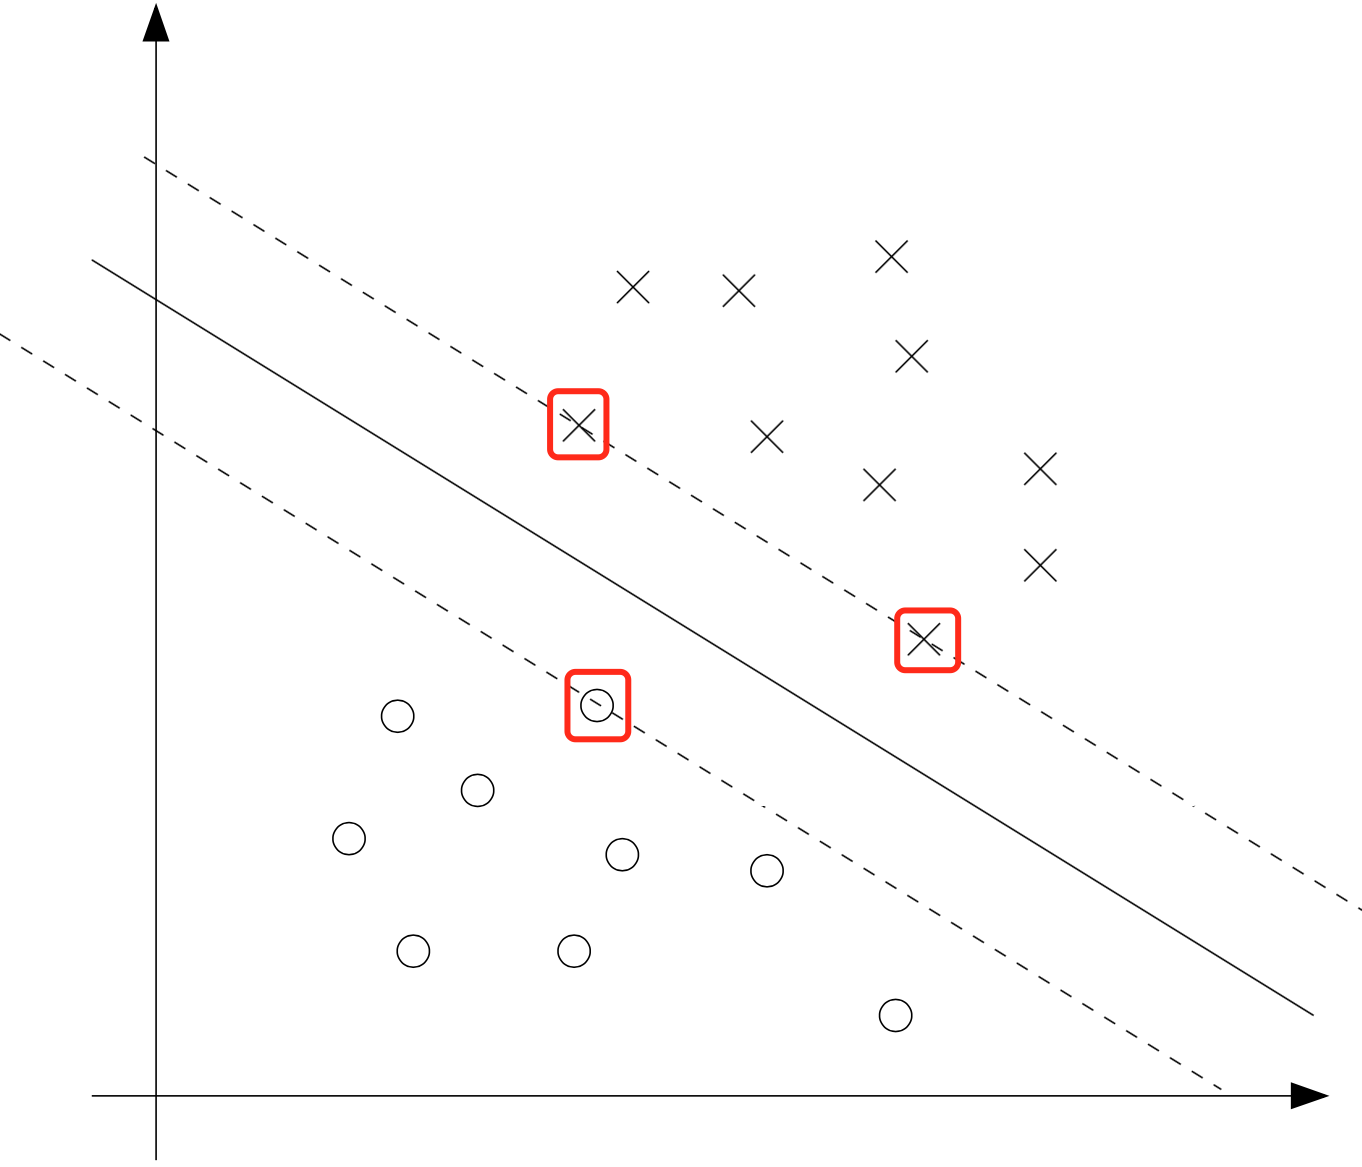
\includegraphics[scale=0.35]{images/支撑向量}
		\caption{支撑向量}
	\end{figure}

	\item 拉格朗日函数为:
	\begin{align}
		\mathcal{L}(w, b, \alpha) = \frac{1}{2}\|w\|^2 - \sum_{i=1}^{m}\alpha_i \left[y^{(i)}(w^Tx^{(i)}+b)-1\right]
	\end{align}
	注意,因为在我们的问题中没有等式约束,故上式没有$\beta_i$。

	\item 接下来我们对拉格朗日函数求偏导数,令偏导数的值为0。
	\begin{align}
		\nabla_{w}\mathcal{L}(w,b,\alpha)=w - \sum_{i=1}^{m}\alpha_iy^{(i)}x^{(i)}=0
	\end{align}
	可得:
	\begin{align}
		w = \sum_{i=1}^{m}\alpha_iy^{(i)}x^{(i)}
		\label{$w$}
	\end{align}
	对$b$:
	\begin{align}
		\frac{\partial}{\partial b}\mathcal{L}(w,b,a) = \sum_{i=1}^{m}a_iy^{(i)}=0
		\label{b}
	\end{align}
	将\ref{$w$}代入拉格朗日函数,得:
	\begin{align}
		\mathcal{L}(w,b,\alpha) = \sum_{i=1}^{m}\alpha_i-\frac{1}{2}\sum_{i,j=1}^{m}y^{(i)}y^{(j)}\alpha_i\alpha_j (x^{(i)})^Tx^{(j)} - b\sum_{i=1}^{m}a_iy^{(i)}
	\end{align}
	再将\ref{b}代入上式,得到:
	\begin{align}
		\mathcal{L}(w,b,\alpha) = \sum_{i=1}^{m}\alpha_i-\frac{1}{2}\sum_{i,j=1}^{m}y^{(i)}y^{(j)}\alpha_i\alpha_j (x^{(i)})^Tx^{(j)}
	\end{align}
	\item 下面我们考虑原问题的对偶优化问题,即:
	\begin{align}
		&\text{优化目标:} \\
		& \qquad \max_{\alpha} W(\alpha) = \sum_{i=1}^{m}\alpha_i-\frac{1}{2}\sum_{i,j=1}^{m}y^{(i)}y^{(j)}\alpha_i\alpha_j \langle x^{(i)}, x^{(j)}\rangle \\
		&\text{约束条件:} \\
		& \qquad \alpha_i \geq 0, \quad i=1,\dots,m \\
		& \qquad \sum_{i=1}^{m}\alpha_iy^{(i)} = 0
	\end{align}
	其中,$\langle x^{(i)}, x^{(j)}\rangle $表示内积\\
	第一个约束是我们一直有的,第二个约束通过求$b$的偏导数后得到\footnote{吴恩达在视频中解释这个约束说明的意义:若$\sum_{i=1}^{m}\alpha_iy^{(i)} \neq 0$,则$\theta_{\mathcal{D}}(\alpha)=-\infty$,所以,如果我们要$\max \theta_{\mathcal{D}}(\alpha)$,就应该取那些能让$\sum_{i=1}^{m}\alpha_iy^{(i)} = 0$的$\alpha$,这样,$\theta_{\mathcal{D}}(\alpha)=W(\alpha)$。{\color{red}{我也没怎么懂,待后面研究研究}}}。

	\item 若要得到$w$,根据公式\ref{$w$},我们可以知道,只要求得了$\alpha$就能得到$w$

	\item 在开始计算前,我们再仔细看下公式\ref{$w$},$w$是关于$\alpha$的函数,我们将其代入$w^Tx+b$后可以发现:
	\begin{align}
		w^Tx + b &= \left( \sum_{i=1}^{m}\alpha_i y^{(i)}x^{(i)} \right)^Tx + b \\
		&= \sum_{i=1}^{m}\alpha_iy^{(i)}\langle x^{(i)}, x \rangle + b \\
		&\downarrow	\\
		h_{w,b}(x) &= g(w^Tx + b) \\
		&= g(\sum_{i=1}^{m}\alpha_iy^{(i)}\langle x^{(i)}, x \rangle + b)
	\end{align}
	前面我们已经讨论过了,除了支撑向量对应的那几个点之外,其余的点$\alpha_i$均为0,而支撑向量的数目很少,这将大大简化我们的计算。

	\item 假设我们已经得到了$w^*$,我们便得到了一堆的平行线(因为决策边界只剩截距$b$不知道了),我们自然会取两类点中间的直线,这样才能保证离每一类都最远,于是:
	\begin{align}
		b^* = - \frac{\max_{i;y^{(i)}=-1}w^*x^{(i)} + \max_{i;y^{(i)}=1}w^*x^{(i)}}{2}
	\end{align}


\end{enumerate}


















			\subsection{核}
为方便后续内容的理解,我先大体讲一下下面的内容: \\

在我们碰到的问题中,有些在低维下不是线性可分的,但是其在高维下却是线性可分的,于是,我们可以将低维下的特征映射到高维中,然后再高维下进行分割,这里的从低维映射到高维就是的方法就是我们后面会提到的$\phi(x)$;但是,这又会带来一个问题,那就是,映射到高维后,如果仅仅制作映射而不做其他优化,我们计算的时间复杂度就上去了,于是我们就想办法来对计算方法进行改善,这个改善的方法就是使用核函数!通过使用核函数,我们并不需要知道我们从低维映射到高维到底是如何映射的(即我们并不显示地知道$\phi(x)$长什么样,我们只知道通过核函数可以达到与通过$\phi(x)$映射后一样的结果)。 \\

简而言之,引出$\phi(\cdot)$是为了说明低维不可分割的数据在高维可能可以分割;再举一堆例子说明通过得到$\phi(\cdot)$后再求$\phi(\cdot)$内积的方式计算量太大,不可取,有更好的计算方式,那就是使用核函数$K(x, z)$\\

按我个人的经验,吴恩达的视频在你还搞不明白核函数的内容时都听不懂他在讲什么,但是在搞明白后就觉得讲得很清晰(也不排除我没认真听......),可以先参考下下面的这篇博文:\url{http://blog.pluskid.org/?p=685} \\

下面开始正文

\subsubsection{特征映射与核函数引入}
\begin{enumerate}
	\item 在前面的线性回归中,我们提到,为了得到更好的拟合结果,我们可以添加高阶项如$x^2, x^3$等来优化拟合结果。为了区分远有的$x$,以及我们添加的$x^2, x^3, ...$,我们将原有的$x$称为问题的{\color{blue}{属性}},将新添加的$x^2, x^3,...$以及$x$一起称为问题的{\color{blue}{特征}}。从$x \to \left[\begin{matrix}x \\ x^2 \\ x^3\end{matrix}\right]$称为特征映射。记为$\phi$,如本例子中:$\phi(x) = \left[\begin{matrix}x \\ x^2 \\ x^3\end{matrix}\right]$

	\item 在前面的算法中,我们可以将内积$\langle x, z \rangle$改为$\langle \phi(x), \phi(x) \rangle$,我们将其定义为高斯函数:
	\begin{align}
		K(x, z) = \phi(x)^T \phi(z)
	\end{align}

	\item 但是,在映射后$\phi(x)^T \phi(z)$的计算量太大,比如
	\begin{enumerate}
		\item 我们先定义一个核函数$K(x, z)=(x^T z)^2$,然后找出其特征映射$\phi(x)$,以此说明若要显式地写出$\phi(x)$的式子与只知道核函数不使用显式的$\phi(x)$两者间的计算量差异。
		\item 对$K(x, z)$进一步计算
		\begin{align}
			K(x, z) &= \left(\sum_{i=1}^{n}x_iz_i \sum_{j=1}^{n}x_jz_j \right) \\
			&= \sum_{i=1}^{n} \sum_{j=1}^{n} x_i x_j z_i z_j \\
			&= \sum_{i,j=1}^{n}(x_i x_j) (z_i z_j)
		\end{align}
		如上,以$n=3$为例,若要将$K(x, z)$表示成$\phi(x)^T\phi(z)$的形式:
		\begin{align}
			\phi(x) = \left[\begin{matrix}x_1 x_1 \\ x_1 x_2 \\ x_1 x_3 \\ x_2 x_1 \\ x_2 x_2 \\ x_2 x_3 \\ x_3 x_1 \\ x_3 x_2 \\ x_3 x_3 \\\end{matrix}\right]
		\end{align}
		$\phi(z)$同理。显然,在上面的$\phi(x)$中,若要讲$x \to \phi(x)$,我们需要进行9次的计算;
		\item 但是,若我们不管$\phi(x)$应如何表示,直接先计算$x^Tz$后再取平方,$n=3$时只需要计算3次。
		\item 实际上,此处的$K(x, z) = (x^T z)^2$ 是我们后面会讲到的多项式核$K(x,z)=\left(\langle x, z \rangle +R \right)^d = \left(x^Tz +R\right)^d$的一种。虽然核函数$K(x,z)$可以很容易地表示出来,但是其特征映射$\phi(x)$却不见得容易表示。
	\end{enumerate}

	\item 所以,虽然前面使用将$x$映射到高维$\phi(x)$来说明这样做可以将低维无法线性分隔的点分隔开,但是在实际计算中,我们并不会去计算$\phi(x)$应如何表示,相当于我们实际上使用更容易计算的核函数$K(x, z)$来达到特征映射$\phi(x)$将低维映射到高维的效果

	\item 我们会做的是找到一个核函数,证明它确实对应着存在一个特征映射$\phi(x)$可以实现将数据在高维特征下分割开。

	\item 注: 下面说明下\url{http://blog.pluskid.org/?p=685}中的例子应如何理解
	\begin{enumerate}
		\item 例子中说明提到:$\phi(\cdot)$的目的是使得向量$x_1=(\eta_1, \eta_2)^T, x_2=(\xi_1, \xi_2)^T$在经过$\phi(\cdot)$映射后再求内积的结果为:
		\begin{align}
			\langle \phi(x_1), \phi(x_2) \rangle = \eta_1\xi_1 + \eta_1^2\xi_1^2 + \eta_2\xi_2 + \eta_2^2\xi_2^2 + \eta_1\eta_2\xi_1\xi_2
		\end{align}
		\item 但是,若我们不知道$\phi(\cdot)$是何种形式,直接通过某个核函数$K(x_1, x_2)$也可以得到同样的结果:
		\begin{align}
			\left( \langle x_1, x_2 \rangle +1 \right)^2 &= \langle x_1, x_2 \rangle ^2 + 2 \langle x_1, x_2 \rangle + 1 \\
			&= (x_1^T x_2)^2 + 2x_1^T x_2 + 1 \\
			&=\left\{ \left[\begin{matrix}\eta_1 & \eta_2\end{matrix}\right]\left[\begin{matrix}\xi_1 \\ \xi_2\end{matrix}\right] \right\}^2 + 2\left[\begin{matrix}\eta_1 & \eta_2\end{matrix}\right]\left[\begin{matrix}\xi_1 \\ \xi_2\end{matrix}\right] + 1 \\
			&= (\eta_1\xi_1+\eta_2\xi_2)^2 + 2(\eta_1\xi_1+\eta_2\xi_2) + 1 \\
			&= \eta_1^2\xi_1^2 + \eta_2^2\xi_2^2 + 2\eta_1\eta_2\xi_1\xi_2 + 2\eta_1\xi_1 + 2\eta_2\xi_2 + 1 \\
		\end{align}
		与前面的式子相比,只要对某些维度进行线性缩放即可,说明两者可以达到同样的效果。
		\item 但是,在计算量上,用第一种方法我们需要先找到其对应的$\phi(\cdot)$(若$\phi(x_1, x-2)=(\sqrt{2}x_1, x_1^2, \sqrt{2}x_2, x_2^2, \sqrt{2}x_1x_2, 1)^T$则可得到与$\left( \langle x_1, x_2 \rangle +1 \right)^2$一样的结果),然后再计算$\phi(\cdot)$的内积。显然,通过$\phi(\cdot)$的方式计算量太大,但是使用核函数计算的方式计算量就小多了。这就是该例子的目的
	\end{enumerate}

	\item 对$\phi(\cdot)$的一个直观但可能不是太准确的描述:对于$\phi(x)$和$\phi(z)$,如果两者比较相近,则其核函数$K(x,z)=\phi(x)^T\phi(z)$值较大;若干两者相差较远,则其结果值较小。所以我们可以将核函数$K(x,z)$看成是对$x,z$有多相近的一种表示。
\end{enumerate}

\subsubsection{常用核函数介绍}
\begin{enumerate}
	\item 多项式核
	\begin{align}
		K(x_1, x_2) = \left(\langle x_1, x_2 \rangle + R\right)^d
	\end{align}
	\item 高斯核
	\begin{align}
		K(x_1, x_2) = e^{-\frac{\|x_1 - x_2\|^2}{2\sigma^2}}
	\end{align}
	高斯核会将原始空间映射到无穷维空间。如果$\sigma$选得很大,高次特征上得权重就衰减得非常快,类似于一个低维的子空间;若$\sigma$选得很小,则可将任意的数据映射为线性可分,不过这可能会带来严重的过拟合问题。\\
	通过调整参数$\sigma$,高斯核具有很高的灵活性,它也是使用最广泛的核函数之一。
	\item 线性核
	\begin{align}
		K(x_1, x_2) = \langle x_1, x_2 \rangle
	\end{align}
	这实际上就是原始空间上的内积。
\end{enumerate}

\subsubsection{核函数需要满足的条件}
\begin{enumerate}
	\item 核矩阵
	对于一个有$\{x^{(1)}, x^{(2)}, \dots, x^{(m)}\}$个数据点的数据集,我们定义核矩阵中的某一项$K_{ij}$为:
	\begin{align}
		K_{ij} = K(x^{(i)}, x^{(j)})
	\end{align}
	核矩阵是一个$m\times m$矩阵
	\item 如果$K$是一个满足条件的(合法的)核函数,则
	\begin{align}
		K_{ij} = K(x^{(i)}, x^{(j)}) = \phi(x^{(i)})^T\phi(x^{(j)}) = \phi(x^{(j)})^T\phi(x^{(i)}) = K(x^{(j)}, x^{(i)}) = K_{ji}
	\end{align}
	所以说,一个合法的核函数要求其核矩阵是对称的。
	\item 用$\phi_k(x)$表示向量$\phi(x)$的第$k$项
	\begin{align}
		z^TKz &= \sum_{i}\sum_{j}z_j K_{ij} z_j \\
		&= \sum_{i}\sum_{j} z_i \phi(x^{(i)})^T \phi(x^{(j)}) z_j \\
		&= \sum_{i}\sum_{j}z_i \sum_{k}\phi_k(x^{(i)})\phi_k(x^{(j)})z_j \\
		&= \sum_{k}\sum_{i}\sum_{j}z_i \phi_k(x^{(i)}) \phi_k(x^{(j)}) z_j \\
		&= \sum_{k} \left(\sum_{i}z_i \phi_k(x^{(i)}) \right)^2 \\
		& \geq 0
	\end{align}
	所以,一个合法的核函数要求其核矩阵是半正定矩阵
	\item 综上,如果一个核函数是合法的,那么我们要求其对应的核矩阵应是一个对称半正定矩阵。我们将其称为Mercer条件,具体表述如下:
	\item Mercer条件
	略
	\item 虽然我们对核函数的推导、引入都是在SVM中进行,但是核函数并不仅仅能用在SVM中,在我们前面讲到的线性回归,逻辑回归中,若我们将式子改写成内积的形式,然后再讲内积替换为核函数的方法,就能够在其他算法中使用核函数了。
\end{enumerate}



		\section{附录}
\subsection{概念与定义}
\subsubsection{各类变量}
\begin{enumerate}
	\item $i$: 第$i$个数据集,从1开始,截止于m
	\item $j$: 第$j$维特征,从0开始,截止于n
	\item $m$: 数据集大小,共$m$组数据
	\item $n$: 维度大小,共$n$维特征
	\item $i, j, m, n$的关系: $\sum_{i=1}^{m}\sum_{j=0}^{j=n}{\theta_{j}x_j^{(i)}}$
	\item $(x^{(i)}, y^{(i)})$: 第i个训练集
	\item $P(y|x;\theta)$中,$y$作为一个个体。$x$作为一个个体。$;\theta$作为一个个体,表示$P(y|x)$以$\theta$为参数
	\item 先验概率: 事情还没有发生,要求这件事情发生的可能性的大小,是先验概率. 
	\item 后验概率: 事情已经发生,要求这件事情发生的原因是由某个因素引起的可能性的大小,是后验概率.
\end{enumerate}

\subsubsection{充分统计量}
\begin{enumerate}
	\item 不损失信息的统计量就是充分统计量,它概括了样本中所包含的未知参数的全部信息。
	\item 定义: 设$x_1, x_2, \dots, x_n$是来自某个总体$X$的样本,总体的分布函数为$F(x;\theta)$,若统计量$T=T(x_1, x_2, \dots, x_n)$为$\theta$的{\color{blue}{充分统计量}},则在给定了$T$的取值后,$x_1, x_2, \dots, x_n$的条件分布$P(X_1=x_1, X_2=x_2, \dots, X_n=x_n$与$\theta$无关
	\item 充分统计量不唯一。实际上,样本本身就是参数的一个充分统计量
	\item 因子分解定理{\color{red}{(没看懂)}}: 设总体的概率函数为$p(x;\theta)$,$x_1, x_2, \dots, x_n$是来自总体的样本,则统计量$T=T(x_1, x_2, \dots, x_n)$为充分统计量的充要条件为:
	\begin{equation}
		p(x_1, x_2, \dots, x_n;\theta) = g\left[T(x_1, x_2, \dots, x_n),\theta\right]\cdot h(x_1, x_2, \dots, x_n)
	\end{equation}
	其中,$g(t,\theta)$是通过统计量T的取值而依赖于样本的,而$h(x_1, x_2, \dots, x_n)$不依赖于$\theta$
\item 更详细内容: \url{http://wenku.baidu.com/view/8813423343323968011c92ed.html}
\end{enumerate}

\subsubsection{自然参数}
\begin{enumerate}
	\item {\color{red}{待补充}}
\end{enumerate}

\subsubsection{先验概率 \& 后验概率}
\begin{enumerate}
	\item 先验概率: 事情还没有发生,要求这件事情发生的可能性的大小,是先验概率. 
	\item 后验概率: 事情已经发生,要求这件事情发生的原因是由某个因素引起的可能性的大小,是后验概率.
\end{enumerate}

\subsubsection{似然函数}
\begin{enumerate}
	\item 似然函数的定义:给定$x$时,关于参数$\theta$的似然函数$L(\theta)$(在数值上)等于给定$\theta$后变量$X=x$的概率:
	\begin{equation}
		L(\theta|x) = P(X=x|\theta)
	\end{equation}
	\item 从定义上讲,似然函数和概率密度函数是两个不同的数学对象,前者是关于未知参数$\theta$的函数,后者是关于$x$的函数。两者的相等仅仅是在数值上的相等。
	\item 似然函数$L(\theta|x)$表示的意义是:在参数$\theta$下,随机变量$X$取到$x$的可能性有多大;概率密度$f(x|\theta)$表示的意义是:在给定样本$x$时,参数$\theta$为真实值的可能性有多大。二者表示的都是可能性。
	\item 若$X$是一个离散型随机变量,则$f(x|\theta)$可改写成$f(x|\theta)=P_\theta(X=x)$。式子$L(\theta_1|x)=P_{\theta_1}(X=x) > L(\theta_2|x)=P_{\theta_2}(X=x)$表示:在参数$\theta_1$下,随机变量$X$取到$x$的可能性大于参数$\theta_2$下随机变量$X$取到$x$的可能性,即$\theta_1$比$\theta_2$更可能是真实值。
	\item 若$X$是一个连续型随机变量也类似。
	\item 参考资料:\href{https://www.zhihu.com/question/54082000}{如何理解似然函数?-知乎} \\
	\href{http://baike.baidu.com/subview/1864828/1864828.htm}{似然函数-百度百科}
\end{enumerate}

\subsubsection{参数学习算法 \& 非参数学习算法}
\begin{enumerate}
	\item 参数学习算法: 对于线性回归算法,一旦拟合出适合训练数据的参数$\theta$,保存这些参数$\theta$,对于之后的预测,不需要再使用原始训练数据集; 
	\item 非参数学习算法: 对于局部加权线性回归算法,每次进行预测都需要全部的训练数据(每次进行的预测得到不同的参数$\theta$),没有固定的参数$\theta$
\end{enumerate}


\subsubsection{Hessian矩阵}
\begin{enumerate}
	\item Hessian矩阵又成海森矩阵
	\item 雅克比(Jacobian)矩阵:多元函数对各自变量的一阶导数
	\begin{align}
	J_F(x_1, \dots, x_n) = 
		\left[\begin{matrix}
			\frac{\partial y_1(x)}{\partial x_1} & \dots & \frac{\partial y_1(x)}{\partial x_n} \\
			\vdots & \ddots & \vdots \\
			\frac{\partial y_m(x)}{\partial x_1} & \dots & \frac{\partial y_m(x)}{\partial x_n}
		\end{matrix}\right]
	\end{align}
	\item 海森矩阵:多元函数对各自变量的二阶导数
	\begin{align}
		H(f) = 
		\left[\begin{matrix}
			\frac{\partial^2 f(x)}{\partial^2 x_1} & \frac{\partial^2 f(x)}{\partial x_1\partial x_2}& \dots & \frac{\partial^2 f(x)}{\partial x_1\partial x_n} \\
			\frac{\partial^2 f(x)}{\partial x_2\partial x_1} & \frac{\partial^2 f(x)}{\partial^2 x_2}& \dots & \frac{\partial^2 f(x)}{\partial x_2\partial x_n} \\
			\vdots & \vdots & \ddots & \vdots \\
			\frac{\partial^2 f(x)}{\partial x_n\partial x_1} & \frac{\partial^2 f(x)}{\partial x_n\partial x_2}& \dots & \frac{\partial^2 f(x)}{\partial^2 x_n} \\
		\end{matrix}\right]
	\end{align}




	\item 参考资料:\href{http://jacoxu.com/jacobian矩阵和hessian矩阵/}{Jacobian矩阵和Hessian矩阵}
\end{enumerate}








































			\subsection{中英对照表}
\begin{enumerate}
	\item 假设函数 - Hypothesis Function
	\item 学习速率 - Learning Rate
	\item 最小均方 - Least Mean Squares - LMS
	\item 线性回归 - Linear Regression - LR
	\item 逻辑回归 - Logistic Regression - LR
	\item 梯度下降 - Gradient Descent - GD
	\item 随机梯度下降 - Stochastic Gradient Descent - SGD
	\item 局部加权回归 - Local Weight Regression - LWR
	\item 独立同分布 - Independently and Identically Distributed - IID
	\item 广义线性模型 - Generalized Linear Model - GLM
	\item 正则响应函数 - Canonical Response Function
	\item 正则关联函数 - Canonical Link Function
	\item 判别学习算法 - Discriminative Learning Algorithm - DLA
	\item 生成学习算法 - Generative Learning Algorithm - GLA
	\item 朴素贝叶斯 - Naive Bayes
	\item 拉普拉斯平滑 - Laplace Smoothing
	\item  - Generalization Error
	\item 支持向量机 - Support Vector Machine - SVM
	\item 函数间隔 - Functional Margin
	\item 几何间隔 - Geometric Margins
\end{enumerate}
			\subsection{思考}
{\color{red}{以下内容均为个人的思考,不一定是正确的。}}
\begin{enumerate}
	\item 机器学习主要就是围绕几个部分进行各种改进:
	\begin{enumerate}
		\item 决策函数(假设函数):$h_\theta(x)$
		\item 最优化方式:
		\item Cost Function: $J(\theta)$
			\begin{enumerate}
				\item Cost Function仅仅只是一种评价预测值与实际值的方式,就算换种评价方式,差距大的仍旧差距大。表面上看起来通过改进Cost Function并没法得到多少改进,但实际上并非如此
				\item 一方面,通过改进Cost Function,可以在计算预测值与实际值误差时给不同的数据点$(x^{(i)}, y^{(i)})$不同的权重,让较重要的点的有较大权重,较不重要的点权重较小。事实上,局部加权回归就是采用此方式
				\item 另一方面,计算Cost Fuction也是需要计算量的,若采用更简单的计算方式也算对算法的一种优化。{\color{gray}{暂未找到实例}}
			\end{enumerate}
		\item 获取最优解的方式,如梯度下降中使用$\theta_j := \theta_j + \frac{\partial J(\theta)}{\theta_j}$进行迭代
	\end{enumerate}

	\item 线性回归

	\item 逻辑回归

	\item 生成学习算法
	\begin{enumerate}
		\item 随机变量连续时,使用高斯判别分析
		\item 随机变量离散时,使用朴素贝叶斯(拉普拉斯平滑)
	\end{enumerate}


	\item 支持向量机闪光点总结:
	\begin{enumerate}
		\item KKT对偶优化条件$\alpha_i^*g_i(w^*) = 0, \quad i=1, \dots, k$:只需要计算支持向量那一部分数据
		\item 特征映射$\phi(\cdot)$:把低维映射到高维,让低维下非线性可分的数据在高维上线性可分
		\item 核函数$K(x,z)$:让特征映射后的内积容易计算
		\item SMO: 
	\end{enumerate}

\end{enumerate}


















	\part{Coursera机器学习课程笔记}
		% \title{机器学习笔记}
\author{MingShun Wu}
\date{\today}
\maketitle
		% \renewcommand{\contentsname}{目录}
\tableofcontents
\setcounter{tocdepth}{3}
		\section{线性回归(Linear Regression)}
\subsection{各向量形式}
在机器学习中,各个变量在单独出现时均为列向量的形式,但若是以多个向量形成的矩阵形式出现时,均为行向量的形式。\\
以下将会写出各个变量单独出现的情况、各变量以矩阵的形式一起出现的情况。
\begin{enumerate}
\item $\vec{x}$
\begin{equation}
	\vec{x} = \left(\begin{matrix}
				x_0 \\ x_1 \\ x_2 \\ \vdots \\ x_n
			\end{matrix}\right)
			= \left(\begin{matrix}
				1 \\ x_1 \\ x_2 \\ \vdots \\ x_n
			\end{matrix}\right)_{(n+1)*1}
\end{equation}

\item $\vec{\theta}$
\begin{equation}
	\vec{\theta} = \left(\begin{matrix}
					\theta_0 \\ \theta_1 \\ \vdots \\ \theta_n
				\end{matrix}\right)_{(n+1)*1}
\end{equation}

\item $\vec{y}$
\begin{equation}
	\vec{y} = \left(\begin{matrix}
				y
			\end{matrix}\right)_{1*1}
\end{equation}

% \item $h_{\vec{\theta}}(\vec{x})$
% \begin{equation}\begin{aligned}
% 	h_{\vec{\theta}}(\vec{x}) & = \vec{\theta}^{T}\vec{X} = \vec{X}^T\vec{\theta} \\
% 		& = \left( \begin{matrix}
% 			1 & x_1 & x_2 & \dots & x_n
% 			\end{matrix}\right)
% 			\left(\begin{matrix}
% 				\theta_0 \\
% 				\theta_1 \\
% 				\dots \\
% 				\theta_n
% 			\end{matrix}\right) \\
% 		& = \theta_0 + \theta_1x_1 + \theta_2x_2 + \dots + \theta_nx_n
% \end{aligned} \end{equation}
\end{enumerate}

\subsection{批梯度下降}
\subsubsection{各矩阵形式}
下述式子中均为矩阵的形式 \\
\begin{enumerate}
\item $X$
\begin{equation} \begin{aligned}
	X & = \left(\begin{matrix}
			\vec{x}^{(1)} \\ \vec{x}^{(2)} \\ \vec{x}^{(3)} \\ \vdots \\ \vec{x}^{(m)}
		\end{matrix}\right) \\
	& = \left( \begin{matrix}
			x_0^{(1)} & x_1^{(1)} & x_2^{(1)} & x_3^{(1)} & \dots & x_n^{(1)} \\
			x_0^{(2)} & x_1^{(2)} & x_2^{(2)} & x_3^{(2)} & \dots & x_n^{(2)} \\
			x_0^{(3)} & x_1^{(3)} & x_2^{(3)} & x_3^{(3)} & \dots & x_n^{(3)} \\
			\vdots    & \vdots    & \vdots    & \vdots    & \ddots & \vdots   \\
			x_0^{(m)} & x_1^{(m)} & x_2^{(m)} & x_3^{(m)} & \dots & x_n^{(m)} \\
			\end{matrix}\right) \\
	& = \left(\begin{matrix}
			1 & x_1^{(1)} & x_2^{(1)} & x_3^{(1)} & \dots & x_n^{(1)} \\
			1 & x_1^{(2)} & x_2^{(2)} & x_3^{(2)} & \dots & x_n^{(2)} \\
			1 & x_1^{(3)} & x_2^{(3)} & x_3^{(3)} & \dots & x_n^{(3)} \\
			\vdots    & \vdots    & \vdots    & \vdots    & \ddots & \vdots   \\
			1 & x_1^{(m)} & x_2^{(m)} & x_3^{(m)} & \dots & x_n^{(m)} \\
		\end{matrix}\right)_{m*(n+1)}
\end{aligned} \end{equation}

\item $\vec{\theta}$
\begin{equation} \begin{aligned}
	\vec{\theta} & = \left(\begin{matrix}
			\theta_0 \\ \theta_1 \\ \theta_2 \\ \theta_3 \\ \vdots \\ \theta_n \\
		\end{matrix}\right)_{(n+1)*1}
\end{aligned}\end{equation}

\item $h_{\vec{\theta}}(\vec{x})$
\begin{equation}\begin{aligned}
	h_{\vec{\theta}}(\vec{x}) &= X * \vec{\theta} \\
	    & = \left(\begin{matrix}
			1 & x_1^{(1)} & x_2^{(1)} & x_3^{(1)} & \dots & x_n^{(1)} \\
			1 & x_1^{(2)} & x_2^{(2)} & x_3^{(2)} & \dots & x_n^{(2)} \\
			1 & x_1^{(3)} & x_2^{(3)} & x_3^{(3)} & \dots & x_n^{(3)} \\
			\vdots    & \vdots    & \vdots    & \vdots    & \ddots & \vdots   \\
			1 & x_1^{(m)} & x_2^{(m)} & x_3^{(m)} & \dots & x_n^{(m)} \\
		\end{matrix}\right)
		\left(\begin{matrix}
			\theta_0 \\ \theta_1 \\ \theta_2 \\ \theta_3 \\ \vdots \\ \theta_n \\
		\end{matrix}\right) \\
		& = \left(\begin{matrix}
			1\theta_0 + x_1^{(1)}\theta_1 + x_2^{(1)}\theta_2 + x_3^{(1)}\theta_3 + \dots + x_n^{(1)}\theta_n \\
			1\theta_0 + x_1^{(2)}\theta_1 + x_2^{(2)}\theta_2 + x_3^{(2)}\theta_3 + \dots + x_n^{(2)}\theta_n \\
			1\theta_0 + x_1^{(3)}\theta_1 + x_2^{(3)}\theta_2 + x_3^{(3)}\theta_3 + \dots + x_n^{(3)}\theta_n \\
			\vdots \\
			1\theta_0 + x_1^{(m)}\theta_1 + x_2^{(m)}\theta_2 + x_3^{(m)}\theta_3 + \dots + x_n^{(m)}\theta_n \\
		\end{matrix}\right)_{m*1}
\end{aligned}\end{equation}

\item $\vec{y}$
\begin{equation}
	\vec{y} = \left(\begin{matrix}
		y^{(1)} \\ y^{(2)} \\ y^{(3)} \\ \vdots \\ y^{(m)}
	\end{matrix}\right)_{m*1}
\end{equation}
\end{enumerate}

\subsubsection{Cost Function}
\begin{enumerate}
\item 数值计算形式:
\begin{equation}
	J(\theta) = \frac{1}{2m} \sum_{i=1}^m \left[ h_\theta(x^{(i)}) - y^{(i)}\right]^2
\end{equation}

\item 矩阵计算形式:
\begin{equation}
	J(\theta) = \frac{1}{2m} \left[h_{\vec{\theta}}(\vec{x}) - \vec{y}\right]^T \left[ h_{\vec{\theta}}(\vec{x}) - \vec{y}\right]
\end{equation}
\end{enumerate}


\subsubsection{偏导数$\frac{\partial J(\theta)}{\partial \theta_j}$计算}
\begin{enumerate}
\item 数值计算形式
\begin{equation}
	\frac{\partial J(\theta)}{\partial \theta_j} =
	    \frac{1}{m} \left[ h_\theta(x^{(i)}) - y^{(i)} \right] x_j^{(i)}
\end{equation}

\item 矩阵计算形式
\begin{equation}
	\nabla J(\theta) = \frac{1}{m} X^T \left[h_{\vec{\theta}}(\vec{x}) - \vec{y}\right]
\end{equation}
\end{enumerate}


\subsubsection{梯度下降迭代方式}
\begin{enumerate}
\item 数值计算形式
\begin{equation}\begin{aligned}
	\theta_j &:= \theta_j - \alpha\frac{\partial J(\theta)}{\partial \theta_j} \\
		&:= \theta_j - \alpha \frac{1}{m} \left[h_\theta(x^{(i)}) - y^{(i)}\right] x_j^{(i)} \\
\end{aligned}\end{equation}

\item 矩阵计算形式
\begin{equation}\begin{aligned}
	\theta &:= \theta - \alpha\nabla J(\theta) \\
		&:= \theta - \alpha \frac{1}{m} X^T \left[ h_{\vec{\theta}}(\vec{x}) - \vec{y}\right]
\end{aligned}\end{equation}
\end{enumerate}



\subsection{Feature Normalization}
\begin{equation}
	x_i = \frac{x_i - \mu}{\sigma}
\end{equation}
或
\begin{equation}
	x_i = \frac{x_i - \mu}{max - min}
\end{equation}



\subsection{公式法求解(Normal Equation)}
\begin{equation}
	\theta = (X^T X)^{-1} X^T y
\end{equation}
















		\section{逻辑回归(Logistic Regression)}
\subsection{当只有2个类别时,使用1个分类器}

\subsubsection{sigmoid函数}
\begin{equation}
	sigmoid(z) = \frac{1}{1 + e^z}
\end{equation}


\subsubsection{预测函数}
\begin{enumerate}
\item 数值形式
\begin{equation}
	h_\theta(x) = \frac{1}{1 + e^{\theta^T x}}
\end{equation}

\item 矩阵形式
\begin{equation}
	h_\theta(X) = \frac{1}{1 + e^{X \theta}}
\end{equation}
\end{enumerate}


\subsubsection{Cost Function}
\begin{enumerate}
\item 数值形式
\begin{equation}
	J(\theta) = \frac{1}{m}
	    \sum_{i=1}^m \left[ -y^{(i)}log{h_\theta(x^{(i)})} - (1-y^{(i)})log{(1-h_\theta(x^{(i)}))} \right]
\end{equation}

\item 矩阵形式
\begin{equation}
		J(\theta) = \frac{1}{m} \left[-y^T \log{h_\theta(x)} - (1-y^T) \log{(1-h_\theta(x)}\right]
\end{equation}
\end{enumerate}

\subsubsection{偏导数$\frac{\partial J(\theta)}{\partial \theta_j}$}
\begin{enumerate}
\item 数值计算形式
\begin{equation}
	\frac{\partial J(\theta)}{\partial \theta_j} =
	    \frac{1}{m} \sum_{i=1}^m \left[h_\theta(x^{(i)}) - y^{(i)}\right] x_j^{(i)}
\end{equation}

\item 矩阵计算形式
\begin{equation}
	\nabla J(\theta) = \frac{1}{m} X^T \left[h_\theta(x) - y\right]
\end{equation}
\end{enumerate}


\subsubsection{梯度下降迭代算法}
\begin{enumerate}
\item 数值计算形式
\begin{equation}\begin{aligned}
	\theta_j &:= \theta_j - \alpha\frac{\partial J(\theta)}{\partial \theta_j} \\
	    &:= \theta_j - \alpha \frac{1}{m} \sum_{i=1}^m \left[h_\theta(x^{(i)}) - y^{(i)}\right] x_j^{(i)}
\end{aligned}\end{equation}

\item 矩阵计算形式
\begin{equation}\begin{aligned}
	\theta &:= \theta - \alpha\nabla J(\theta) \\
		&:= \theta - \alpha \frac{1}{m} X^T \left[h_\theta(x) - y\right]
\end{aligned}\end{equation}
\end{enumerate}



\subsection{当只有k个类别时,使用k个分类器}
% 当只有k个类别时,使用k个分类器

		\section{Regularization}
\subsection{线性回归}


\subsubsection{数值计算方式}
\begin{equation}
	J(\theta) = \frac{1}{2m}\sum_{i=1}^m [h_\theta(x^{(i)})-y^{(i)}]^2 + \lambda \frac{1}{2m} \sum_{j=1}^n\theta_j^2
\end{equation}

\begin{equation}\begin{aligned}
	\frac{\partial{J(\theta)}}{\partial{\theta_j}} &= \frac{1}{2m}\sum_{i=1}^m 2[h_\theta(x^{(i)}-y^{(i)})] \frac{\partial{h_\theta(x^{(i)})}}{\partial{\theta_j}} + \lambda \frac{1}{2m} 2 \sum_{i=1}^n \theta_j \\
	    &= \frac{1}{m}\sum_{i=1}^m[h_\theta(x^{(i)})-y^{(i)}]x^{(i)} + \frac{\lambda}{m}\sum_{i=1}^n \theta_j
\end{aligned}\end{equation}

\[\begin{cases}
	\theta_0 := \theta_0 - \alpha \frac{1}{m} \sum_{i=1}^m(h_\theta(x^{(i)}) - y^{(i)})x_0^{(i)}, \quad j=0 \\
	\theta_j := \theta_j - \alpha \frac{1}{m} \sum_{i=1}^m(h_\theta(x^{(i)}) - y^{(i)})x_j^{(i)} + \alpha\frac{\lambda}{m}\theta_j, \quad j \neq 0
\end{cases}\]



\subsubsection{矩阵计算方式}
\begin{equation}
	J(\theta) = \frac{1}{2m} \left[h_\theta(x) - y\right]^T \left[ h_\theta(x) - y\right] + \frac{\lambda}{2m} \sum_{j=1}^n\theta_j^2
\end{equation}

\begin{equation}
	\nabla J(\theta) = \frac{1}{2m} X^T \left[h_\theta(x) - y\right] + \frac{\lambda}{m}\sum_{i=1}^n \theta_j
\end{equation}

% \[\begin{cases}
% 	\theta_0 := \theta_0 - \alpha \frac{1}{m} \sum_{i=1}^m(h_\theta(x^{(i)}) - y^{(i)})x_0^{(i)}, \quad j=0 \\
% 	\theta := \theta - \alpha \frac{1}{m} \sum_{i=1}^m(h_\theta(x^{(i)}) - y^{(i)})x^{(i)} + \alpha \frac{\lambda}{m}\theta, \quad j \neq 0
% \end{cases}\]

\[matlab\begin{cases}
	grad &= 1/m * X'*(h-y); , \quad\\
	grad(2:end) &= grad(2:end) + lambda/m * theta(2:end);
\end{cases}\]



\subsection{逻辑回归}

\subsubsection{数值计算方式}
\begin{equation}
	J(\theta) = \frac{1}{m}
	    \sum_{i=1}^m \left[ -y^{(i)}log{h_\theta(x^{(i)})} - (1-y^{(i)})log{(1-h_\theta(x^{(i)}))} \right]
		+ \lambda \frac{1}{2m} \sum_{j=1}^n\theta_j^2
\end{equation}

\[\begin{cases}
	\theta_0 := \theta_0 - \alpha \frac{1}{m} \sum_{i=1}^m(h_\theta(x^{(i)}) - y^{(i)})x_0^{(i)}, \quad j=0 \\
	\theta_j := \theta_j - \alpha \frac{1}{m} \sum_{i=1}^m(h_\theta(x^{(i)}) - y^{(i)})x_j^{(i)} + \alpha\frac{\lambda}{m}\theta_j, \quad j \neq 0
\end{cases}\]

\subsubsection{矩阵计算方式}
\begin{equation}
		J(\theta) = \frac{1}{m} \left[-y^T \log{h_\theta(x)} - (1-y^T) \log{(1-h_\theta(x)}\right] + \lambda \frac{1}{2m}\theta^T \theta
\end{equation}

% \[\begin{cases}
% 	\theta_0 := \theta_0 - \alpha \frac{1}{m} \sum_{i=1}^m(h_\theta(x^{(i)}) - y^{(i)})x_0^{(i)}, \quad j=0 \\
% 	\theta := \theta - \alpha \frac{1}{m} \sum_{i=1}^m(h_\theta(x^{(i)}) - y^{(i)})x^{(i)} + \alpha \frac{\lambda}{m}\theta, \quad j \neq 0
% \end{cases}\]

\[matlab\begin{cases}
	grad &= 1/m * X'*(h-y); , \quad\\
	grad(2:end) &= grad(2:end) + lambda/m * theta(2:end);
\end{cases}\]



\subsection{注意}
在实际计算$\theta$中,都是先计算没有Regularization的结果,再对(2:end)计算有Regularization的结果,再将其加到没有Regularization的结果中







		\section{神经网络--前向算法}

\subsection{神经网络示意图--前向算法}
\begin{tikzpicture}
\tikzset{
	a/.style={circle, draw=black}
}

% x
% \node[a] (x_0) at(0,10) {$x_0=+1$};
\node[a] (x_1) at(0,8) {$x_1$};
\node[a] (x_2) at(0,6) {$x_2$};
\node[a] (x_3) at(0,4) {$x_3$};
\filldraw (0,3) circle (.06);
\filldraw (0,2) circle (.06);
\filldraw (0,1) circle (.06);
\node[a] (x_n) at(0,0) {$x_n$};

% X与a的分隔线
\draw [dashed] (1,-1) -- (1,9);

% a^{(1)}
\node[a] (a_10) at(2,10)   {$+1$};
\node[a] (a_11) at(2,8)   {$a_1^{(1)}$};
\node[a] (a_12) at(2,6) {$a_2^{(1)}$};
\node[a] (a_13) at(2,4)   {$a_3^{(1)}$};
\filldraw (2,3) circle (.06);
\filldraw (2,2) circle (.06);
\filldraw (2,1) circle (.06);
\node[a] (a_1s1) at(2,0) {$a_{s_1}^{(1)}$};

% a^{(2)}
\node[a] (a_20) at(6,9.5) {$+1$};
\node[a] (a_21) at(6,8.0) {$a_1^{(2)}$};
\node[a] (a_22) at(6,6.5) {$a_2^{(2)}$};
\node[a] (a_23) at(6,5.0) {$a_3^{(2)}$};
\node[a] (a_24) at(6,3.5) {$a_4^{(2)}$};
\filldraw (6,2.4) circle (.06);
\filldraw (6,1.8) circle (.06);
\filldraw (6,1.2) circle (.06);
\node[a] (a_2s2) at(6,0) {$a_{s_2}^{(2)}$};

% a^{(3)}
\node[a] (a_30) at(10,9.5) {$+1$};
\node[a] (a_31) at(10,8.0) {$a_1^{(3)}$};
\node[a] (a_32) at(10,6.5) {$a_2^{(3)}$};
\node[a] (a_33) at(10,5.0) {$a_3^{(3)}$};
\node[a] (a_34) at(10,3.5) {$a_4^{(3)}$};
\filldraw (10,2.4) circle (.06);
\filldraw (10,1.8) circle (.06);
\filldraw (10,1.2) circle (.06);
\node[a] (a_3s3) at(10,0) {$a_{s_3}^{(3)}$};

% 中间部分
\filldraw (12,0) circle (.06);
\filldraw (12,2) circle (.06);
\filldraw (12,4) circle (.06);
\filldraw (12,6) circle (.06);
\filldraw (12,8) circle (.06);

% a^{(n)}

\node[a] (a_L1) at(14,7.5) {$a_1^{(L)}$};
\node[a] (a_L2) at(14,6)   {$a_2^{(L)}$};
\node[a] (a_L3) at(14,4.5) {$a_3^{(L)}$};
\node[a] (a_L4) at(14,3)   {$a_4^{(L)}$};
\filldraw (14,2.0) circle (.06);
\filldraw (14,1.5) circle (.06);
\filldraw (14,1.0) circle (.06);
\node[a] (a_Lsl) at(14,0) {$a_{s_l}^{(L)}$};


% 前向算法图例--仅连线:a1 -- a_21
% \draw[->] (a_10) -- (a_21);
\draw[->] (a_11) -- (a_21);
\draw[->] (a_12) -- (a_21);
\draw[->] (a_13) -- (a_21);
% \draw[->] (a_1s1) -- (a_21);

% 前向算法图例--有标注:a1 -- a_21
\path (a_10) edge[->] node[auto] {$\theta_{10}^{(1)}$} (a_21);
% \path (a_11) edge[->] node[auto] {$\theta_{11}^{(1)}$} (a_21);
% \path (a_12) edge[->] node[auto] {$\theta_{12}^{(1)}$} (a_21);
% \path (a_13) edge[->] node[auto] {$\theta_{13}^{(1)}$} (a_21);
\path (a_1s1) edge[->] node[auto] {$\theta_{1s1}^{(1)}$} (a_21);


% 前向算法--仅连线: a2 --> a34
% \draw[->] (a_20) -- (a_34);
\draw[->] (a_21) -- (a_34);
\draw[->] (a_22) -- (a_34);
\draw[->] (a_23) -- (a_34);
\draw[->] (a_24) -- (a_34);
% \draw[->] (a_2s2) -- (a_34);

% 前后算法图例--有标注:a2 -- a34
\path (a_20) edge[->] node[auto] {$\theta_{40}^{(2)}$} (a_34);
% \path (a_21) edge[->] node[auto] {$\theta_{41}^{(2)}$} (a_34);
% \path (a_22) edge[->] node[auto] {$\theta_{42}^{(2)}$} (a_34);
% \path (a_23) edge[->] node[auto] {$\theta_{43}^{(2)}$} (a_34);
% \path (a_24) edge[->] node[auto] {$\theta_{44}^{(2)}$} (a_34);
\path (a_2s2) edge[->] node[auto] {$\theta_{4s2}^{(2)}$} (a_34);


% 下方的标志
\node at (4, 11) {\color{red}{$\Theta^{(1)}$}};
\node at (8, 11) {\color{red}{$\Theta^{(2)}$}};

\end{tikzpicture}


\begin{equation}
	a^{(j)} = g(z^{(j-1)}) \Rightarrow {(m,s_j)}
\end{equation}

\begin{equation}
	\Theta^{(j)} = 
		\left(\begin{matrix}
			\theta_{10}^{(j)} & \theta_{11}^{(j)} & \theta_{12}^{(j)} & \dots & \theta_{1,s_{j}}^{(j)} \\
			\theta_{20}^{(j)} & \theta_{21}^{(j)} & \theta_{22}^{(j)} & \dots & \theta_{2,s_{j}}^{(j)} \\
			\theta_{30}^{(j)} & \theta_{31}^{(j)} & \theta_{32}^{(j)} & \dots & \theta_{3,s_{j}}^{(j)} \\
			\vdots    & \vdots    & \vdots    & \ddots & \vdots   \\
			\theta_{s_{j+1}0}^{(j)} & \theta_{s_{j+1}1}^{(j)} & \theta_{s_{j+1}2}^{(j)} & \dots & \theta_{s_{j+1},s_{j}}^{(j)}
		\end{matrix}\right) \Rightarrow {(s_{j+1},s_{j}+1)}
\end{equation}

\begin{equation}\begin{aligned}
	z^{(j+1)} &= (1, a^{(j)}) (\Theta^{(j)})^T \\
		\\ &= 
			\left(\begin{matrix}
				z_1^{(j+1)(1)} & z_2^{(j+1)(1)} & z_3^{(j+1)(1)} & \dots & z_{s_{j+1}}^{(j+1)(1)} \\
				z_1^{(j+1)(2)} & z_2^{(j+1)(2)} & z_3^{(j+1)(2)} & \dots & z_{s_{j+1}}^{(j+1)(2)} \\
				z_1^{(j+1)(3)} & z_2^{(j+1)(3)} & z_3^{(j+1)(3)} & \dots & z_{s_{j+1}}^{(j+1)(3)} \\
				\vdots & \vdots & \vdots & \ddots & \vdots \\
				z_1^{(j+1)(m)} & z_2^{(j+1)(m)} & z_3^{(j+1)(m)} & \dots & z_{s_{j+1}}^{(j+1)(m)} \\
			\end{matrix}\right)
\end{aligned}\end{equation}

\begin{equation}
	a^{(j+1)} = g(z^{(j+1)})  \Rightarrow {(m,s_{j+1})} 
\end{equation}


\begin{equation} \begin{aligned}
	y & = \left(\begin{matrix}
			y^{(1)} \\ y^{(2)} \\ y^{(3)} \\ \vdots \\ y^{(m)} \\
		\end{matrix}\right)_{m*1}
\end{aligned} \end{equation}

		\subsection{神经网络--前向算法}

\subsubsection{$X、\theta、\Theta、z、a$}
\begin{enumerate}
\item X
\begin{equation} \begin{aligned}
	X & = \left(\begin{matrix}
			(x^{(1)})^T \\ (x^{(2)})^T \\ (x^{(3)})^T \\ \vdots \\ (x^{(m)})^T \\
		\end{matrix}\right) \\
	& = \left( \begin{matrix}
			x_1^{(1)} & x_2^{(1)} & x_3^{(1)} & \dots & x_n^{(1)} \\
			x_1^{(2)} & x_2^{(2)} & x_3^{(2)} & \dots & x_n^{(2)} \\
			x_1^{(3)} & x_2^{(3)} & x_3^{(3)} & \dots & x_n^{(3)} \\
			\vdots    & \vdots    & \vdots    & \ddots & \vdots   \\
			x_1^{(m)} & x_2^{(m)} & x_3^{(m)} & \dots & x_n^{(m)} \\
			\end{matrix}\right) \\
	& = \left(\begin{matrix}
			x_1^{(1)} & x_2^{(1)} & x_3^{(1)} & \dots & x_n^{(1)} \\
			x_1^{(2)} & x_2^{(2)} & x_3^{(2)} & \dots & x_n^{(2)} \\
			x_1^{(3)} & x_2^{(3)} & x_3^{(3)} & \dots & x_n^{(3)} \\
			\vdots    & \vdots    & \vdots    & \ddots & \vdots   \\
			x_1^{(m)} & x_2^{(m)} & x_3^{(m)} & \dots & x_n^{(m)} \\
		\end{matrix}\right) \Rightarrow {(m,n)}
\end{aligned} \end{equation}

\item $a^{(1)}$
\begin{equation}
	a^{(1)} = X  \Rightarrow {(m,n)}
\end{equation}

\item $\Theta^{(1)}$
\begin{equation}
\Theta^{(1)} = 
	\left(\begin{matrix}
		\theta_{10}^{(1)} & \theta_{11}^{(1)} & \theta_{12}^{(1)} & \dots & \theta_{1,s_1}^{(1)} \\
		\theta_{20}^{(1)} & \theta_{21}^{(1)} & \theta_{22}^{(1)} & \dots & \theta_{2,s_1}^{(1)} \\
		\theta_{30}^{(1)} & \theta_{31}^{(1)} & \theta_{32}^{(1)} & \dots & \theta_{3,s_1}^{(1)} \\
		\vdots    & \vdots    & \vdots    & \ddots & \vdots   \\
		\theta_{s_{2}0}^{(1)} & \theta_{s_{2}1}^{(1)} & \theta_{s_{2}2}^{(1)} & \dots & \theta_{s_{2},s_{1}}^{(1)}
	\end{matrix}\right) \Rightarrow {(s_{2},s_1+1)=(s_{2},n+1)}
\end{equation}

\item $z^{(2)}$ \\
给$a^{(1)}$的每个数据均添加上$a_0 = 1$后与$\Theta^{(1)}$计算,得到$z^{(2)}
\footnote{从$a^{(1)}$得到$a^{(2)}$需要经过sigmoid()函数,后续的从$a^{(j)}$得到$a^{(j+1)}$均需要经过sigmoid()函数}
=(1, a^{(1)})(\Theta^{(1)})^T$
\begin{equation}\begin{aligned}
	z^{(2)} &= (1, a^{(1)}) (\Theta^{(1)})^T \Rightarrow (m,n+1) * (n+1,s_{2})
		\\ &= 
		  \left(\begin{matrix}
				1 & x_1^{(1)} & x_2^{(1)} & x_3^{(1)} & \dots & x_n^{(1)} \\
				1 & x_1^{(2)} & x_2^{(2)} & x_3^{(2)} & \dots & x_n^{(2)} \\
				1 & x_1^{(3)} & x_2^{(3)} & x_3^{(3)} & \dots & x_n^{(3)} \\
				\vdots        & \vdots    & \vdots    & \vdots    & \ddots & \vdots   \\
				1 & x_1^{(m)} & x_2^{(m)} & x_3^{(m)} & \dots & x_n^{(m)} \\
			\end{matrix}\right)
			\left(\begin{matrix}
				\theta_{10}^{(1)} & \theta_{11}^{(1)} & \theta_{12}^{(1)} & \dots & \theta_{1,n}^{(1)} \\
				\theta_{20}^{(1)} & \theta_{21}^{(1)} & \theta_{22}^{(1)} & \dots & \theta_{2,n}^{(1)} \\
				\theta_{30}^{(1)} & \theta_{31}^{(1)} & \theta_{32}^{(1)} & \dots & \theta_{3,n}^{(1)} \\
				\vdots    & \vdots    & \vdots    & \ddots & \vdots   \\
				\theta_{s_{2},0}^{(j)} & \theta_{s_{2},1}^{(j)} & \theta_{s_{2},2}^{(j)} & \dots & \theta_{s_{2},n}^{(1)}
			\end{matrix}\right)^T
		\\ &= 
		  \left(\begin{matrix}
				1 & x_1^{(1)} & x_2^{(1)} & x_3^{(1)} & \dots & x_n^{(1)} \\
				1 & x_1^{(2)} & x_2^{(2)} & x_3^{(2)} & \dots & x_n^{(2)} \\
				1 & x_1^{(3)} & x_2^{(3)} & x_3^{(3)} & \dots & x_n^{(3)} \\
				\vdots        & \vdots    & \vdots    & \vdots    & \ddots & \vdots   \\
				1 & x_1^{(m)} & x_2^{(m)} & x_3^{(m)} & \dots & x_n^{(m)} \\
			\end{matrix}\right)
			\left(\begin{matrix}
				\theta_{10}^{(1)} & \theta_{20}^{(1)} & \theta_{30}^{(1)} & \dots & \theta_{s_{2},0}^{(1)} \\
				\theta_{11}^{(1)} & \theta_{21}^{(1)} & \theta_{31}^{(1)} & \dots & \theta_{s_{2},1}^{(1)} \\
				\theta_{12}^{(1)} & \theta_{22}^{(1)} & \theta_{32}^{(1)} & \dots & \theta_{s_{2},2}^{(1)} \\
				\theta_{13}^{(1)} & \theta_{23}^{(1)} & \theta_{33}^{(1)} & \dots & \theta_{s_{2},3}^{(1)} \\
				\vdots    & \vdots    & \vdots    & \ddots & \vdots   \\
				\theta_{1,n}^{(1)} & \theta_{2,n}^{(1)} & \theta_{3,n}^{(1)} & \dots & \theta_{s_{2},n}^{(1)}
			\end{matrix}\right)
		\\ &=
			\left(\begin{matrix}
				z^{(2)(1)} \\ z^{(2)(2)} \\ z^{(2)(3)} \\ \vdots \\ z^{(2)(m)} 
			\end{matrix}\right)
		\\ &= 
			\left(\begin{matrix}
				z_1^{(2)(1)} & z_2^{(2)(1)} & z_3^{(2)(1)} & \dots & z_{s_2}^{(2)(1)} \\
				z_1^{(2)(2)} & z_2^{(2)(2)} & z_3^{(2)(2)} & \dots & z_{s_2}^{(2)(2)} \\
				z_1^{(2)(3)} & z_2^{(2)(3)} & z_3^{(2)(3)} & \dots & z_{s_2}^{(2)(3)} \\
				\vdots & \vdots & \vdots & \ddots & \vdots \\
				z_1^{(2)(m)} & z_2^{(2)(m)} & z_3^{(2)(m)} & \dots & z_{s_2}^{(2)(m)} \\
			\end{matrix}\right)
		\\ &  \Rightarrow  (m,n+1) * (n+1, s_{2}) = (m,s_2)
\end{aligned}\end{equation}
\footnote{上式$z_{s_2}^{(2)(m)}$中,$(2)$表示第2层神经网络,$(m)$表示第m个训练集,$s_2$表示第2层神经网络的最后一个单元}


\item $a^{(2)}$
\begin{equation}
	a^{(2)}=g(z^{(2)}) \Rightarrow {(m,s_2)}
\end{equation}

\item 后续同理 \\
\begin{equation}\begin{aligned}
	\Theta^{(2)} &= 
		\left(\begin{matrix}
			\theta_{10}^{(2)} & \theta_{11}^{(2)} & \theta_{12}^{(2)} & \dots & \theta_{1,s_2}^{(2)} \\
			\theta_{20}^{(2)} & \theta_{21}^{(2)} & \theta_{22}^{(2)} & \dots & \theta_{2,s_2}^{(2)} \\
			\theta_{30}^{(2)} & \theta_{31}^{(2)} & \theta_{32}^{(2)} & \dots & \theta_{3,s_2}^{(2)} \\
			\vdots    & \vdots    & \vdots    & \ddots & \vdots   \\
			\theta_{s_{3}0}^{(2)} & \theta_{s_{3}1}^{(2)} & \theta_{s_{3}2}^{(2)} & \dots & \theta_{s_{3},s_{2}}^{(2)}
		\end{matrix}\right) \Rightarrow {(s_{3},s_2+1)}\\
	z^{(3)} &= (1, a^{(2)}) (\Theta^{(2)})^T \Rightarrow (m,s_2+1) * (s_2+1, s_3) = (m,s_3) \\
	a^{(3)} &= g(z^{(3)}) \Rightarrow {(m,s_3)} \\
	& \vdots \\
\end{aligned} \end{equation}

\item 一般式
\begin{equation}\begin{aligned}
	a^{(j)} &= g(z^{(j-1)}) \Rightarrow {(m,s_j)} \\
	\Theta^{(j)} &= 
		\left(\begin{matrix}
			\theta_{10}^{(j)} & \theta_{11}^{(j)} & \theta_{12}^{(j)} & \dots & \theta_{1,s_{j}}^{(j)} \\
			\theta_{20}^{(j)} & \theta_{21}^{(j)} & \theta_{22}^{(j)} & \dots & \theta_{2,s_{j}}^{(j)} \\
			\theta_{30}^{(j)} & \theta_{31}^{(j)} & \theta_{32}^{(j)} & \dots & \theta_{3,s_{j}}^{(j)} \\
			\vdots    & \vdots    & \vdots    & \ddots & \vdots   \\
			\theta_{s_{j+1}0}^{(j)} & \theta_{s_{j+1}1}^{(j)} & \theta_{s_{j+1}2}^{(j)} & \dots & \theta_{s_{j+1},s_{j}}^{(j)}
		\end{matrix}\right) \Rightarrow {(s_{j+1},s_{j}+1)}\\
	z^{(j+1)} &= (1, a^{(j)}) (\Theta^{(j)})^T \\
		% \\ &= 
		%   \left(\begin{matrix}
		% 		1 & x_1^{(1)} & x_2^{(1)} & x_3^{(1)} & \dots & x_n^{(1)} \\
		% 		1 & x_1^{(2)} & x_2^{(2)} & x_3^{(2)} & \dots & x_n^{(2)} \\
		% 		1 & x_1^{(3)} & x_2^{(3)} & x_3^{(3)} & \dots & x_n^{(3)} \\
		% 		\vdots        & \vdots    & \vdots    & \vdots    & \ddots & \vdots   \\
		% 		1 & x_1^{(m)} & x_2^{(m)} & x_3^{(m)} & \dots & x_n^{(m)} \\
		% 	\end{matrix}\right)
		% 	\left(\begin{matrix}
		% 		\theta_{10}^{(1)} & \theta_{11}^{(1)} & \theta_{12}^{(1)} & \dots & \theta_{1,n}^{(1)} \\
		% 		\theta_{20}^{(1)} & \theta_{21}^{(1)} & \theta_{22}^{(1)} & \dots & \theta_{2,n}^{(1)} \\
		% 		\theta_{30}^{(1)} & \theta_{31}^{(1)} & \theta_{32}^{(1)} & \dots & \theta_{3,n}^{(1)} \\
		% 		\vdots    & \vdots    & \vdots    & \ddots & \vdots   \\
		% 		\theta_{s_{2},0}^{(j)} & \theta_{s_{2},1}^{(j)} & \theta_{s_{2},2}^{(j)} & \dots & \theta_{s_{2},n}^{(1)}
		% 	\end{matrix}\right)^T
		\\ &= 
		  \left(\begin{matrix}
				1 & a_1^{(j)(1)} & a_2^{(j)(1)} & a_3^{(j)(1)} & \dots & a_{s_j}^{(j)(1)} \\
				1 & a_1^{(j)(2)} & a_2^{(j)(2)} & a_3^{(j)(2)} & \dots & a_{s_j}^{(j)(2)} \\
				1 & a_1^{(j)(3)} & a_2^{(j)(3)} & a_3^{(j)(3)} & \dots & a_{s_j}^{(j)(3)} \\
				\vdots        & \vdots    & \vdots    & \vdots    & \ddots & \vdots   \\
				1 & a_1^{(j)(m)} & a_2^{(j)(m)} & a_3^{(j)(m)} & \dots & a_{s_j}^{(j)(m)} \\
			\end{matrix}\right)
			\left(\begin{matrix}
				\theta_{10}^{(j)} & \theta_{20}^{(j)} & \theta_{30}^{(j)} & \dots & \theta_{s_{j+1},0}^{(j)} \\
				\theta_{11}^{(j)} & \theta_{21}^{(j)} & \theta_{31}^{(j)} & \dots & \theta_{s_{j+1},1}^{(j)} \\
				\theta_{12}^{(j)} & \theta_{22}^{(j)} & \theta_{32}^{(j)} & \dots & \theta_{s_{j+1},2}^{(j)} \\
				\theta_{13}^{(j)} & \theta_{23}^{(j)} & \theta_{33}^{(j)} & \dots & \theta_{s_{j+1},3}^{(j)} \\
				\vdots    & \vdots    & \vdots    & \ddots & \vdots   \\
				\theta_{1,s_j}^{(j)} & \theta_{2,s_j}^{(j)} & \theta_{3,s_j}^{(j)} & \dots & \theta_{s_{j+1},s_j}^{(j)}
			\end{matrix}\right)
		\\ &=
			\left(\begin{matrix}
				z^{(j+1)(1)} \\ z^{(j+1)(2)} \\ z^{(j+1)(3)} \\ \vdots \\ z^{(j+1)(m)} 
			\end{matrix}\right)
		\\ &= 
			\left(\begin{matrix}
				z_1^{(j+1)(1)} & z_2^{(j+1)(1)} & z_3^{(j+1)(1)} & \dots & z_{s_{j+1}}^{(j+1)(1)} \\
				z_1^{(j+1)(2)} & z_2^{(j+1)(2)} & z_3^{(j+1)(2)} & \dots & z_{s_{j+1}}^{(j+1)(2)} \\
				z_1^{(j+1)(3)} & z_2^{(j+1)(3)} & z_3^{(j+1)(3)} & \dots & z_{s_{j+1}}^{(j+1)(3)} \\
				\vdots & \vdots & \vdots & \ddots & \vdots \\
				z_1^{(j+1)(m)} & z_2^{(j+1)(m)} & z_3^{(j+1)(m)} & \dots & z_{s_{j+1}}^{(j+1)(m)} \\
			\end{matrix}\right)
		\\ & \Rightarrow (m,s_j+1) * (s_j+1, s_{j+1}) = (m,s_{j+1}) \\
	a^{(j+1)} &= g(z^{(j+1)})  \Rightarrow {(m,s_{j+1})} 
\end{aligned}\end{equation}
\end{enumerate}

\subsubsection{y}
\begin{equation} \begin{aligned}
	y & = \left(\begin{matrix}
			y^{(1)} \\ y^{(2)} \\ y^{(3)} \\ \vdots \\ y^{(m)} \\
		\end{matrix}\right)_{m*1}
\end{aligned} \end{equation}

为进行矩阵运算,要将其转化为如下形式:\footnote{y所对应的值所在的索引位置值为1,其他位置均为0}
\begin{equation}\begin{aligned}
	Y &= \left(\begin{matrix}
	        0 & 0 & 0 & \dots & 0 & 1 \\
	        0 & 1 & 0 & \dots & 0 & 0 \\
	        0 & 0 & 1 & \dots & 0 & 0 \\
	        \vdots & \vdots & \vdots & \vdots & \ddots & \vdots \\
	        1 & 0 & 0 & \dots & 0 & 0 \\
		\end{matrix}\right)_{m,s_L}
\end{aligned}\end{equation}\footnote{上式$m*s_L$中的$s_L$表示共有$s_L$个分类器,$s_L$表示的是输出层的unit数}

		\section{神经网络--后向算法}

\subsection{神经网络示意图--后向算法}
\begin{tikzpicture}
\tikzset{
	a/.style={circle, draw=black}
}

% x
% \node[a] (x_0) at(0,10) {$x_0=+1$};
\node[a] (x_1) at(0,8) {$x_1$};
\node[a] (x_2) at(0,6) {$x_2$};
\node[a] (x_3) at(0,4) {$x_3$};
\filldraw (0,3) circle (.06);
\filldraw (0,2) circle (.06);
\filldraw (0,1) circle (.06);
\node[a] (x_n) at(0,0) {$x_n$};

% X与a的分隔线
\draw [dashed] (1,-1) -- (1,9);

% \delta^{(1)}
\node[a] (a_10) at(2,10)   {0};
\node[a] (a_11) at(2,8)   {0};
\node[a] (a_12) at(2,6) {0};
\node[a] (a_13) at(2,4)   {0};
\filldraw (2,3) circle (.06);
\filldraw (2,2) circle (.06);
\filldraw (2,1) circle (.06);
\node[a] (a_1s1) at(2,0) {0};

% \delta^{(2)}
\node[a] (a_20) at(6,9.5) {$\delta_0^{(2)}$};
\node[a] (a_21) at(6,8.0) {$\delta_1^{(2)}$};
\node[a] (a_22) at(6,6.5) {$\delta_2^{(2)}$};
\node[a] (a_23) at(6,5.0) {$\delta_3^{(2)}$};
\node[a] (a_24) at(6,3.5) {$\delta_4^{(2)}$};
\filldraw (6,2.4) circle (.06);
\filldraw (6,1.8) circle (.06);
\filldraw (6,1.2) circle (.06);
\node[a] (a_2s2) at(6,0) {$\delta_{s_2}^{(2)}$};

% \delta^{(3)}
\node[a] (a_30) at(10,9.5) {$\delta_0^{(3)}$};
\node[a] (a_31) at(10,8.0) {$\delta_1^{(3)}$};
\node[a] (a_32) at(10,6.5) {$\delta_2^{(3)}$};
\node[a] (a_33) at(10,5.0) {$\delta_3^{(3)}$};
\node[a] (a_34) at(10,3.5) {$\delta_4^{(3)}$};
\filldraw (10,2.4) circle (.06);
\filldraw (10,1.8) circle (.06);
\filldraw (10,1.2) circle (.06);
\node[a] (a_3s3) at(10,0) {$\delta_{s_3}^{(3)}$};

% 中间部分
\filldraw (12,0) circle (.06);
\filldraw (12,2) circle (.06);
\filldraw (12,4) circle (.06);
\filldraw (12,6) circle (.06);
\filldraw (12,8) circle (.06);

% \delta^{(n)}

\node[a] (a_L1) at(14,7.5) {$\delta_1^{(L)}$};
\node[a] (a_L2) at(14,6)   {$\delta_2^{(L)}$};
\node[a] (a_L3) at(14,4.5) {$\delta_3^{(L)}$};
\node[a] (a_L4) at(14,3)   {$\delta_4^{(L)}$};
\filldraw (14,2.0) circle (.06);
\filldraw (14,1.5) circle (.06);
\filldraw (14,1.0) circle (.06);
\node[a] (a_Lsl) at(14,0) {$\delta_{s_l}^{(L)}$};


% % 后向算法图例--仅连线:\delta21 -- \delta_1
% \draw[->] (a_21) -- (a_10);
% \draw[->] (a_21) -- (a_11);
% \draw[->] (a_21) -- (a_12);
% \draw[->] (a_21) -- (a_13);
% \draw[->] (a_21) -- (a_1s1);
% % 后向算法图例--仅连线:\delta22 -- \delta_1
% \draw[->] (a_22) -- (a_10);
% \draw[->] (a_22) -- (a_11);
% \draw[->] (a_22) -- (a_12);
% \draw[->] (a_22) -- (a_13);
% \draw[->] (a_22) -- (a_1s1);
% % 后向算法图例--仅连线:\delta23 -- \delta_1
% \draw[->] (a_23) -- (a_10);
% \draw[->] (a_23) -- (a_11);
% \draw[->] (a_23) -- (a_12);
% \draw[->] (a_23) -- (a_13);
% \draw[->] (a_23) -- (a_1s1);
% % 后向算法图例--仅连线:\delta24 -- \delta_1
% \draw[->] (a_24) -- (a_10);
% \draw[->] (a_24) -- (a_11);
% \draw[->] (a_24) -- (a_12);
% \draw[->] (a_24) -- (a_13);
% \draw[->] (a_24) -- (a_1s1);
% % 后向算法图例--仅连线:\delta2s2 -- \delta_1
% \draw[->] (a_2s2) -- (a_10);
% \draw[->] (a_2s2) -- (a_11);
% \draw[->] (a_2s2) -- (a_12);
% \draw[->] (a_2s2) -- (a_13);
% \draw[->] (a_2s2) -- (a_1s1);


% 后向算法--仅连线: \delta31 --> \delta2
\draw[->] (a_31) -- (a_20);
\draw[->] (a_31) -- (a_21);
\draw[->] (a_31) -- (a_22);
\draw[->] (a_31) -- (a_23);
\draw[->] (a_31) -- (a_24);
\draw[->] (a_31) -- (a_2s2);
% 后向算法--仅连线: \delta32 --> \delta2
\draw[->] (a_32) -- (a_20);
\draw[->] (a_32) -- (a_21);
\draw[->] (a_32) -- (a_22);
\draw[->] (a_32) -- (a_23);
\draw[->] (a_32) -- (a_24);
\draw[->] (a_32) -- (a_2s2);
% 后向算法--仅连线: \delta33 --> \delta2
\draw[->] (a_33) -- (a_20);
\draw[->] (a_33) -- (a_21);
\draw[->] (a_33) -- (a_22);
\draw[->] (a_33) -- (a_23);
\draw[->] (a_33) -- (a_24);
\draw[->] (a_33) -- (a_2s2);
% 后向算法--仅连线: \delta34 --> \delta2
\draw[->] (a_34) -- (a_20);
\draw[->] (a_34) -- (a_21);
\draw[->] (a_34) -- (a_22);
\draw[->] (a_34) -- (a_23);
\draw[->] (a_34) -- (a_24);
\draw[->] (a_34) -- (a_2s2);
% 后向算法--仅连线: \delta3s3 --> \delta2
\draw[->] (a_3s3) -- (a_20);
\draw[->] (a_3s3) -- (a_21);
\draw[->] (a_3s3) -- (a_22);
\draw[->] (a_3s3) -- (a_23);
\draw[->] (a_3s3) -- (a_24);
\draw[->] (a_3s3) -- (a_2s2);


% 标志
\node at (4, 11) {$\Theta^{(1)}$};
\node at (8, 11) {$\Theta^{(2)}$};
\node at (2, -1) {\color{red}{无$\delta^{(1)}$}};
\node at (6, -1) {\color{red}{$\delta^{(2)}$}};
\node at (10, -1) {\color{red}{$\delta^{(3)}$}};


% \node at (4, -2) {\color{red}{$\delta^{(1)}=(\Theta^{(1)})^T [\delta^{2}(2:end)] .* g(z^{1}) .* (1-g(z^{1}))$}};
% \node at (8, -3) {\color{red}{$\delta^{(l)}=(\Theta^{(l)})^T [\delta^{l+1}(2:end)] .* g(z^{l}) .* (1-g(z^{l}))$}};


\end{tikzpicture}



\[\begin{cases}
	\delta^{L} &= a^{L} - y ,\quad l=L \\
	\delta^{L-1} &= (\Theta^{(L-1)})^T \delta^{L} .* g^{'}(z^{L-1}) \\
		&= (\Theta^{(L-1)})^T \delta^{L} .* g(z^{L-1}) .* (1-g(z^{L-1})),\quad l=L-1 \\
		\delta^{l} &= (\Theta^{(l)})^T [\delta^{l+1}(2:end)] .* g^{'}(z^{l}) \\
	&= (\Theta^{(l)})^T [\delta^{l+1}(2:end)] .* g(z^{l}) .* (1-g(z^{l})) ,\quad 2<=l<=L-2 \\
	% 无 a^{(1)}, \quad l=1
\end{cases}\] \\
无 $\delta^{(1)}$

\begin{equation}\begin{aligned}
		\Delta^{(l)} := \Delta^{(l)} + \delta^{(l+1)} (a^{(l)})^T
	\end{aligned}\end{equation}

\[ D_{ij}^{(l)} = \begin{cases}
	\frac{1}{m}\Delta_{ij}^{(l)} ,\quad j=0 \\
	\frac{1}{m}(\Delta_{ij}^{(l)} + \Theta_{ij}^{(l)}), \quad j \neq 0
\end{cases}\]

\begin{equation*}
	\frac{\partial{J(\Theta)}}{\partial{\Theta_{ij}^{(l)}}} = D_{ij}^{(l)}
\end{equation*}





		\subsection{神经网络--后向算法}

\subsubsection{输出层结果:$a^L$}
\begin{equation}
	a^L = 
		\left(\begin{matrix}
			a_1^{(L)(1)} & a_2^{(L)(1)} & a_3^{(L)(1)} & \dots & a_{s_L}^{(L)(1)} \\
			a_1^{(L)(2)} & a_2^{(L)(2)} & a_3^{(L)(2)} & \dots & a_{s_L}^{(L)(2)} \\
			a_1^{(L)(3)} & a_2^{(L)(3)} & a_3^{(L)(3)} & \dots & a_{s_L}^{(L)(3)} \\
			\vdots & \vdots & \vdots & \ddots & \vdots \\
			a_1^{(L)(m)} & a_2^{(L)(m)} & a_3^{(L)(m)} & \dots & a_{s_L}^{(L)(m)} \\
		\end{matrix}\right)_{m,s_L}
\end{equation}

\subsubsection{格式化后的Y}
\begin{equation}\begin{aligned}
	Y &= \left(\begin{matrix}
	        0 & 0 & 0 & \dots & 0 & 1 \\
	        0 & 1 & 0 & \dots & 0 & 0 \\
	        0 & 0 & 1 & \dots & 0 & 0 \\
	        \vdots & \vdots & \vdots & \vdots & \ddots & \vdots \\
	        1 & 0 & 0 & \dots & 0 & 0 \\
		\end{matrix}\right)_{m,s_L}
\end{aligned}\end{equation}

\subsubsection{$\delta^{L}$}
\begin{equation}\begin{aligned}
	\delta^{L} &= a^{L} - y \\
		&= \left(\begin{matrix}
			a_1^{(L)} \\ a_2^{(L)} \\ a_3^{(L)} \\ \vdots \\ a_{s_L}^{(L)}
		\end{matrix}\right) - 
		\left(\begin{matrix}
	        1 \\ 0 \\ 0 \\ \vdots \\ 0 \\ 0 
		\end{matrix}\right)
\end{aligned}\end{equation}
\begin{itemize}
	\item 此时,$\delta^{L}, a^{L}, y$表示的是均向量(不是矩阵)
\end{itemize}

% \begin{equation}\begin{aligned}
% 	\Delta^{L} &= a^{L} - Y \\
% 	&= 	
% 		\left(\begin{matrix}
% 			a_1^{(L)(1)} & a_2^{(L)(1)} & a_3^{(L)(1)} & \dots & a_{s_L}^{(L)(1)} \\
% 			a_1^{(L)(2)} & a_2^{(L)(2)} & a_3^{(L)(2)} & \dots & a_{s_L}^{(L)(2)} \\
% 			a_1^{(L)(3)} & a_2^{(L)(3)} & a_3^{(L)(3)} & \dots & a_{s_L}^{(L)(3)} \\
% 			\vdots & \vdots & \vdots & \ddots & \vdots \\
% 			a_1^{(L)(m)} & a_2^{(L)(m)} & a_3^{(L)(m)} & \dots & a_{s_L}^{(L)(m)} \\
% 		\end{matrix}\right) - 
% 		 \left(\begin{matrix}
% 	        0 & 0 & 0 & \dots & 0 & 1 \\
% 	        0 & 1 & 0 & \dots & 0 & 0 \\
% 	        0 & 0 & 1 & \dots & 0 & 0 \\
% 	        \vdots & \vdots & \vdots & \vdots & \ddots & \vdots \\
% 	        1 & 0 & 0 & \dots & 0 & 0 \\
% 		\end{matrix}\right)_{m,s_L}
% \end{aligned}\end{equation}
% \begin{itemize}
% 	\item 此时,$\Delta^{L}, a^{L}, Y$表示的是均是矩阵
% 	\item {\color{red}{从教程看,似乎不用这样算,都用迭代的方式,这大概也是$\delta^{l}$ 与 $\Delta^{l}$表示的意义不一样的来源}}
% \end{itemize}

\subsubsection{$\delta^{L-1}$}
\begin{equation}\begin{aligned}
	\delta^{L-1} &= (\Theta^{(L-1)})^T \delta^{L} .* g^{'}(z^{L-1}) \\
	&= (\Theta^{(L-1)})^T \delta^{L} .* g(z^{L-1}) .* (1-g(z^{L-1}))
\end{aligned}\end{equation}
\begin{enumerate}
	\item 其中,式$g^{'}(z) = g(z)(1-g(z))$,此为sigmoid()函数的特性
	\item 此时,$z^{L-1}$表示的是一个向量(不是矩阵)
	\item 此时不需要舍弃$\delta_0^{L}$,因为根本就没有
\end{enumerate}

% \begin{equation}\begin{aligned}
% 	\Delta^{L-1} &= (\Theta^{(L-1)})^T \Delta^{L} .* g^{'}(z^{L-1}) \\
% 	&= (\Theta^{(L-1)})^T \Delta^{L} .* g(z^{L-1}) .* (1-g(z^{L-1}))
% \end{aligned}\end{equation}
% \begin{enumerate}
% 	\item 此时,$z^{L-1}$表示的是矩阵
% 	\item 与上述的$\delta^{L-1}$相比,此式批量计算的训练集中的所有数据
% 	\item {\color{red}{从教程看,似乎不用这样算,都用迭代的方式,这大概也是$\delta^{l}$ 与 $\Delta^{l}$表示的意义不一样的来源}}
% \end{enumerate}


\subsubsection{$\delta^{l}$($2<=l<=L-2$)}
\begin{equation}\begin{aligned}
	\delta^{l} &= (\Theta^{(l)})^T [\delta^{l+1}(2:end)] .* g^{'}(z^{l}) \\
	&= (\Theta^{(l)})^T [\delta^{l+1}(2:end)] .* g(z^{l}) .* (1-g(z^{l}))
\end{aligned}\end{equation}
\begin{enumerate}
	\item 因$a^{(1)}$直接从X得到,不会有误差,故无$\delta^{(1)}$
	\item (2:end)表示舍弃第一个数据$\delta_0^{s_{L-1}}$(Matlab索引从1开始)
	\item 对比于从$a^{l}$到$a^{l+1}$要添加一个$a_0^{l}=1$;从$\delta^{l+1}$到$\delta^{l}$要舍弃一个$\delta_0^{l+1}$
	\item 同样地,此时$z^{l}$表示的是一个向量(不是矩阵)
\end{enumerate}

\subsubsection{$\Delta^{l}$(用迭代的方式计算)}
\begin{enumerate}
	\item 数值计算方式
	\begin{equation}\begin{aligned}
		\Delta_{ij}^{(l)} := \Delta_{ij}^{(l)} + a_j^{(l)} \delta_i^{(l+1)}
	\end{aligned}\end{equation}
	\item 矩阵计算方式
	\begin{equation}\begin{aligned}
		\Delta^{(l)} := \Delta^{(l)} + \delta^{(l+1)} (a^{(l)})^T
	\end{aligned}\end{equation}
\end{enumerate}

\subsubsection{$D_{ij}^{(l)}$}
\begin{enumerate}
	\item $j=0$时
	\begin{equation}
		D_{ij}^{(l)} := \frac{1}{m}\Delta_{ij}^{(l)}
	\end{equation}
	\item $j \neq 0$时
		\begin{equation}
		D_{ij}^{(l)} := \frac{1}{m}(\Delta_{ij}^{(l)} + \Theta_{ij}^{(l)})
	\end{equation}
\end{enumerate}

\subsubsection{$\frac{\partial{J(\Theta)}}{\partial{\Theta_{ij}^{(l)}}}$}
\begin{equation}
	\frac{\partial{J(\Theta)}}{\partial{\Theta_{ij}^{(l)}}} = D_{ij}^{(l)}
\end{equation}

\subsubsection{$\delta^{l}$ 与 $\Delta^{l}$的区别与联系}














		\section{调试技巧}

\subsection{Error Analysis}
\begin{enumerate}
	\item 0-1错分率 or 误分类率
	1. 将当前的数据分成2份,$70\%$作为训练集,$30\%$作为测试集\\
	2. 用新的训练集训练,用新的测试集检验效果\\
	3. 若$J_{train}(\theta)$很小,$J_{test}(\theta)$很大,则说明出现了过拟合
	\item 训练集 \& 交叉验证集 \& 测试集
	\item 过拟合、欠拟合的判断方法
	1. 欠拟合对应高偏差,表现为$J_{cv}(\theta) \approx J_{train}(\theta)$,且二者都很高 \\
	2. 过拟合对应高方差,表现为$J_{cv}(\theta) >> J_{train}(\theta)$,且$J_{train}(\theta)$很小 \\
	3. $J_{taain}(\theta)$对应训练集的学习能力;$J_{cv}(\theta)$对应训练结果对新样本的适应能力,适应能力越强,$J_{cv}(\theta)$越小 \\
	4. 在训练集和验证集(测试集)效果均不好,说明欠拟合;在训练集效果很好,但在说明欠拟合,但在验证集(测试集)效果不好,说明过拟合
\end{enumerate}

\subsection{Error Metrics for Skewed Classes}
\begin{enumerate}
	\item Skewed Classes
	那些两种(或多种)情况发生的概率相关较大的情况称为Skewed Classes。如买彩票中奖的概率与不中奖的概率
	\item True vs. False \& Positive vs. Negative
	Predicted:1, Actual:1 --- True Positive --- TP; \\
	Predicted:0, Actual:0 --- True Negative ---TN; \\
	Predicted:1, Actual:0 --- False Positive --- FP; \\
	Predicted:0, Actual:0 --- False Negative --- FN; \\
	True \& False 对应预测的是否正确; \\
	Positive \& Negative 对应实际是否发生
	\item Accuracy \& Precision \& Recall
	Accuracy: 发生的概率:$\frac{True}{False} = \frac{TP+TN}{TP+TN+FP+FN}$; 
	Precision: 查准率,在预测为1的情况下,实际为1的概率:$frac{TP}{TP+FP}$ \\
	Recall:召回率,在实际为1的情况下,被预测出来的概率: $\frac{TP}{TP+FN}$
	\item Precision \& Recall均是越高越好,但实际上,两者无法同时都很高。(PS:两者加起来并不一定会等于1,甚至很小情况下才全等于1))
\end{enumerate}

\subsection{如何评价Precision与Recall}
\begin{enumerate}
	\item 使用$F_1Score = 2\frac{PR}{P+R}$
	\item 用交叉验证集的$F_1$值来选取最大的$F_1$值对应的P和R,不用训练集(或测试集)中的。
\end{enumerate}



\subsection{拟合效果不好时的解决方法指导}
\begin{enumerate}
	\item 获取更多数据 ---- 解决高方差
	\item 减少特征 ---- 解决高方差
	\item 增加特征 ---- 解决高偏差
	\item 增加高阶多项式 ---- 解决高偏差
	\item 减小$\lambda$ ---- 解决高偏差
	\item 增大$\lambda$ ---- 解决高方差
\end{enumerate}

\subsection{不同神经网络的优缺点}
\begin{enumerate}
	\item 小型神经网络 -- 更少的参数;容易出现欠拟合
	\item 大型神经网络 -- 更多的参数;容易出现过拟合
	\item parameters越复杂,或隐藏的层越多,对训练集的拟合效果越好,但若对验证集的拟合效果不好,说明已经过拟合,此时再增加神经网络的复杂度并不能提高神经网络的效果
\end{enumerate}

\subsection{绘制Learning Curve}
绘制Learning Curve时,对训练集计算训练误差时,每次迭代只能使用训练集的部分数据(第i次迭代使用第1到第i个数据);但对验证集计算验证误差时,每次均应使用所有数据









		\section{SVM}
\subsection{Cost Function}
\begin{equation}\begin{aligned}
	J(\theta) = C\sum_{i=1}^m y^{(i)}cost_1(\theta^Tx^{(i)}) + (1-y^{(i)})cost_0(\theta^Tx^{(i)}) + \frac{1}{2}\sum_{j=1}^n\Theta_j^2
\end{aligned}\end{equation}
其中,$cost_1(\theta^Tx^{(i)})$对应$y=1$; $cost_0(\theta^Tx^{(i)})$对应$y=0$


\subsection{Gaussian Kernel}
\begin{equation}\begin{aligned}
	f_i = similarity(x, l^{(i)}) = exp(-\frac{\sum_{j=1}^n(x_j - l_j^{(i)})^2}{2\sigma^2})
\end{aligned}\end{equation}
\begin{enumerate}
	\item 当$x \approx l^{(i)}$时,$f_i=exp(-\frac{\approx 0^2}{2\sigma^2}) \approx 1$
	\item 当$x$远离$l^{(i)}$时,$f_i=exp(-\frac{inf^2}{2\sigma^2}) \approx 1$
	\item 3
\end{enumerate}





\subsection{SVM中,$C$与$\sigma^2$对欠拟合或过拟合的影响}
\begin{enumerate}
	\item C:C过大:低偏差,高方差;C过小:高偏差,第方差
	\item $\lambda^2$: 过大: 高偏差,低方差;过小: 低偏差,高方差
\end{enumerate}



\subsection{如何选项使用Logistic Regression还是 SVM}
\begin{enumerate}
	\item $n$很大时,使用Logistic Regression或无kernel(即linear kernel)的SVM
	\item $n$很小,$m$中等:使用Gaussian kernel的SVM
	\item $n$很小,$m$很大:增加特征,并使使用Logistic Regression或无kernel(即linear kernel)的SVM
	\item 神经网络可能更加适合,但是使用神经网络训练需要耗费的时间较长
\end{enumerate}


	\part{概率统计基础知识}
		% \title{机器学习笔记}
\author{MingShun Wu}
\date{\today}
\maketitle
		% \renewcommand{\contentsname}{目录}
\tableofcontents
\setcounter{tocdepth}{3}
		\section{随机事件和概率}
\subsection{基本概念及公式}
\begin{enumerate}
	\item 完备事件组 \\
	满足$\cup_{i=1}^nB_i=\Omega$,且$B_iB_j = \emptyset$的事件组$B_1$, $B_2$, ..., $B_n$成为完备事件组
	\item 乘法公式
	\begin{align}
	P(A_1A_2...A_n) &= P(A_1)P(A_2|A_1)P(A_3|A_1A_2)....P(A_n|A_1A_2...A_{n-1})
	\end{align}
	乘法公式并没有$A_k$要相互独立或条件独立的要求。

	\item 全概率公式
	\begin{equation}
	P(A) = \sum_{i=1}^{n}P(A|B_i)P(B_i)
	\end{equation}
	其中,$B$为一完备事件组

	\item 贝叶斯公式
	\begin{align}
	P(B_j|A) &= \frac{P(A|B_j)P(B_j)}{P(A)} \\
	&= \frac{P(A|B_j)P(B_j)}{\sum_{i=1}^{n}P(A|B_i)P(B_i)},  \quad j = 1, 2, 3, ..., n
	\end{align}
	\footnote{$P(B_j|A)=\frac{P(AB_j)}{P(A)}$,再将分子用乘法公式展开,分母用全概率公式展开,即可得到贝叶斯公式} \\
	同样,要求B为完备事件组。 \\
	贝叶斯公式求得是条件概率,求解过程中一般需要用到全概率公式(除非$P(A)$已知)。 \\
	事情还没有发生,要求这件事情发生的可能性的大小,是先验概率;事情已经发生,要求这件事情发生的原因是由某个因素引起的可能性的大小,是后验概率。所以贝叶斯公式求的是后验概率。
	\item 其他
	\begin{enumerate}
		\item 加法公式
		\begin{align}
			P(A\cup B) &= P(A) + P(B) - P(AB) \\
			P(A\cup B\cup C) &= P(A)+P(B)+P(C)-P(AB)-P(BC)-P(AC) +P(ABC)
		\end{align}
		\item 减法公式
		\begin{equation}
			P(A-B) = P(A)-P(AB)
		\end{equation}
	\end{enumerate}
\end{enumerate}

		\section{常用分布}

\subsection{离散型}
\begin{enumerate}
	\item $0-1$分布
	\begin{align}
		P(X=1) &= p \\
		P(X=0) &= 1-p
	\end{align}
	即
	\begin{align}
		P(X=x) = p^x(1-p)^{(1-x)}
	\end{align}
	\footnote{在机器学习中常用此式子表示$0-1$分布}
	\item 二项分布
	\begin{equation}
		P(X=k) = C_n^kp^kq^{n-k}, \quad k=0, 1, 2, \dots, n, \quad q=1-p
	\end{equation}

	\item 几何分布:第$k$次首次发生
	\begin{equation}
		P(X=k) = pq^{k-1}, \quad k=1, 2, 3, ...
	\end{equation}

	\item 超几何分布:共$N$件产品,其中有$M$件次品,共取$n$次,取到$k$件次品
	\begin{equation}
	P(X=k) = \frac{C_M^kC_{N-M}^{n-k}}{C_N^n}, \quad k = l_1, \dots, l_2
	\end{equation}
	其中,$l_1 = max(0, n-N+M\footnote{通过$N-M {\geq} n-k$可以得到})$, $l_2=min(M,n)$

	\item 泊松分布
	\begin{equation}
		P(X=k) = \frac{\lambda^k}{k!}e^{-\lambda}, \quad k=0, 1, 2, \dots
	\end{equation}
	其中,$\lambda>0$且为常数
\end{enumerate}

\subsection{连续型}\footnote{在数学解题中常用分布函数$F(x)$,若有需要再求导得到概率密度;但在机器学习中,常用概率密度函数$f(x)$}
\begin{enumerate}
	\item 连续型随机变量的分布函数$F(x)$必定连续,但是,其概率密度函数$f(x)$不一定连续
	\item 均匀分布
	\[ f(x)=\begin{cases}
	\frac{1}{b-a}, \quad a \leq x \leq b, \\
	0, \quad Others
	\end{cases} \]

	\item 指数分布
	\[ f(x)=\begin{cases}
	\lambda e^{-\lambda x}, \quad x>0, \\
	0, \quad x \leq 0
	\end{cases} \]
	\footnote{对比一下机器学习中的指数分布族:$p(y;\eta) = b(y)e^{\eta^T T(y) - a(\eta)}$,相当于$b(y)=\lambda, \eta^T=-\lambda, T(y)=y, a(\eta)=0$}
	其中,$\lambda>0$。\\
	其分布函数为
	\[ F(x)=\begin{cases}
	1-e^{-\lambda x}, \quad x>0 \\
	0, \quad x \leq 0
	\end{cases} \]

	\item 正态分布
	\begin{equation}
		f(x) = \frac{1}{\sqrt{2\pi} \sigma}e^{-\frac{(x-\mu)^2}{2\sigma^2}}, \quad -\infty < x < +\infty
	\end{equation}
	其分布函数为
	\begin{equation}
		F(x) = \frac{1}{\sqrt{2\pi}\sigma} \int_{-\infty}^x  e^{-\frac{(t-\mu)^2}{2\sigma^2}} dt, \quad -\infty < x < +\infty
	\end{equation}
	标准正态分布
	\begin{equation}
		\Phi(x) = \frac{1}{\sqrt{2\pi}} \int_{-\infty}^x e^{-\frac{t^2}{2}} dt
	\end{equation}
\end{enumerate}

\subsection{泊松定理}
在伯努利实验中,若$n$较大,$p_n$较小,是的$np_n$在$n \to +\infty$时为一常数,则有
\begin{equation}
	\lim_{n \to +\infty}C_n^k p^k (1-p)^{n-k} = \frac{\lambda ^k}{k!}e^{-\lambda}
\end{equation}
其中,$\lim_{n\to+\infty}np = \lambda$







		\section{多维随机变量及其分布}
\subsection{二维随机变量及其分布}
\subsubsection{连续型}
\begin{enumerate}
	\item 二维随机变量的分布
	\begin{equation}
		F(x, y) = P(X\leq x, Y \leq y), \quad -\infty < x < +\infty, -\infty < y < + \infty
	\end{equation}

	\item 二维随机变量的边缘分布
	\begin{equation}\begin{aligned}
			F_X(x) &= P(X\leq x) = P(X\leq x, y< +\infty) = F(x, +\infty) \\
			F_Y(y) &= P(Y\leq y) = P(X< +\infty, Y\leq y) = F(+\infty, y)
	\end{aligned}\end{equation}
	\item 二维随机变量的条件分布
	\begin{align}
		F_{X|Y}(x|y) = P(X \leq x | Y=y) 
		= \lim_{\epsilon \to 0^+}P(X \leq x | y - \epsilon < Y \leq y + \epsilon) \\
		= \lim_{\epsilon \to 0^+} \frac{P(X \leq x, y - \epsilon < Y \leq y + \epsilon)}{P(y - \epsilon < Y \leq y + \epsilon)}
	\end{align}
	$F_{Y|X}(y|x)$同理 \\
	若$f(x,y)$在$(x,y)$点连续,且$f_Y(y)>0$,则:
	\begin{equation}
		F_{X|Y}(x|y) = \int_{-\infty}^{x}\frac{f(s,y)}{f_Y(y)}ds
	\end{equation}
	$F_{Y|X}(y|x)=\int_{-\infty}^{y}\frac{f(x,s)}{f_X(x)}ds$

\end{enumerate}

\subsubsection{离散型}
\begin{enumerate}
	\item 二维离散型随机变量的概率分布(或称分布律)
	\begin{equation}
		P(X=x_i, Y=y_j) = p_{ij}, \quad i,j = 1, 2, \dots
	\end{equation}

	\item 二维离散型随机变量的边缘分布
	\begin{align}
		p_{i\cdot} &= P(X=x_i) 
		= \sum_{j=1}^{+\infty}P(X=x_i, Y=y_j) 
		= \sum_{j=1}^{+\infty}p_{ij}, \quad i = 1, 2, \dots \\
		p_{\cdot j} &= P(Y=y_j) 
		= \sum_{i=1}^{+\infty}P(X=x_i, Y=y_j) 
		= \sum_{i=1}^{+\infty}p_{ij}, \quad j = 1, 2, \dots 
	\end{align}
	\item 二维离散型随机变量的条件分布
	\begin{equation}\begin{aligned}
		P(X=x_i|Y=y_j) = \frac{P(X=x_i, Y=y_j)}{P(Y=y_j)} = \frac{p_{ij}}{p_{\cdot j}}, \quad i = 1, 2, \dots
	\end{aligned}\end{equation}


\end{enumerate}

\subsection{概率密度}
\subsubsection{连续型}
\begin{enumerate}
	\item 二维随机变量及其概率密度 \\
	满足以下条件的$f(x, y)$成为$(X, Y)$的概率密度 \\
	\begin{equation}
		F(x, y) = \int_{-\infty}^{x} \int_{-\infty}^{y}f(u, v)dudv, \quad -\infty <x, y < +\infty
	\end{equation}
	\item 边缘密度
	\begin{equation}
		f_X(x) = \int_{-\infty}^{+\infty}f(x, y)dy
	\end{equation}
	\begin{equation}
		f_Y(y) = \int_{-\infty}^{+\infty}f(x, y)dx
	\end{equation}
	\item 条件密度
	\begin{equation}
		f_{X|Y}(x|y) = \frac{f(x,y)}{F_Y(y)}, \quad f_Y(y) > 0
	\end{equation}
\end{enumerate}

\subsubsection{离散型}
无


\subsection{分布函数与概率密度的性质} % (fold)
\label{sub:性质}
\subsubsection{$F(x,y)$的性质}
\begin{enumerate}
	\item
	\begin{equation}
		F(-\infty, y) = F(x, -\infty) = F(-\infty, \infty) = 0
	\end{equation}
	\begin{equation}
		F(+\infty, +\infty) = 1
	\end{equation}

	\item 
	\begin{equation}
		P(a<X\leq b, c<Y\leq d) = F(b,d) - F(b,c) - F(a,d) + F(a,c)
	\end{equation}
\end{enumerate}

\subsubsection{$P(X=x_i, Y=y_j)=p_{ij}$的性质}
\begin{enumerate}
	\item 
	\begin{equation}
		p_{ij} \geq 0, \quad i,j = 1,2, \dots
	\end{equation}

	\item 
	\begin{equation}
		\sum_i \sum_j p_{ij} = 1
	\end{equation}
\end{enumerate}

\subsubsection{$f(x,y)$的性质}
\begin{enumerate}
	\item 
	\begin{equation}
		f(x, y) \geq 0
	\end{equation}
	\item 
	\begin{equation}
		\int_{-\infty}^{+\infty} \int_{-\infty}^{+\infty}f(x,y)dxdy = 1
	\end{equation}
	\item 
	\begin{equation}
		P((X,y)\in D) = \iint_Df(x,y) dxdy
	\end{equation}
	
\end{enumerate}


\subsection{随机变量的独立性}
\subsubsection{随机变量$X$与$Y${\color{red}{相互独立}}的{\color{red}{充要条件}}}
\begin{enumerate}
	\item 离散型
	\begin{equation}
		P(X=x_i, Y=y_j) = P(X=x_i)P(Y=y_j)
	\end{equation}
	即
	\begin{equation}
		p_{ij} = p_{i\cdot} p_{\cdot j}
	\end{equation}
	\footnote{在机器学习中,若两事件独立,常会用到$P(B|A)=\frac{P(AB)}{P(A)}=\frac{P(A)P(B)}{P(A)}=P(B)$;或$B_k$条件独立时$P(B_2|A, B_1) = P(B_2|A)$}

	\item 连续型
	\begin{equation}
		f(x, y) = f_X(x)f_Y(y)
	\end{equation}
	
\end{enumerate}


\subsection{二维均匀分布\&二维正态分布}
\begin{enumerate}
	\item 二维均匀分布
		\[ f(x, y)=\begin{cases}
			\frac{1}{A}, \quad (x, y) \in G \\
			0, \quad others
		\end{cases} \]

	\item 二维正态分布
	\begin{equation}
		f(x,y) = \frac{1}{2\pi \sigma_1 \sigma_2 \sqrt{1-\rho^2}}e^{-\frac{1}{2(1-\rho^2)}\left[ \frac{(x-\mu_1)^2}{\sigma_1^2} - \frac{2\rho(x-\mu_1)(y-\mu_2)}{\sigma_1 \sigma_2} + \frac{(y-\mu_2)^2}{\sigma_2^2} \right]}, \quad -\infty<x<+\infty, -\infty<y<+\infty
	\end{equation}
	其中,$\mu_1, \mu_2 > 0, \sigma_1>0, \sigma_2 > 0, -1<\rho < 1$,且均为常数,记作
	\begin{equation}
		(X,Y) \sim N(\mu_1, \mu_2; \sigma_1^2, \sigma_2^2; \rho)
	\end{equation}

	\item 若$(X,Y)$二维正态,则$X, Y$均正态,即: 若$(X, Y) \sim N(\mu_1, \mu_2; \sigma_1^2, \sigma_2^2; \rho)$,则$X \sim N(\mu_1, \sigma_1^2), Y \sim N(\mu_2, \sigma_2^2)$
	
	\item 若$(X,Y)$二维正态,则$X, Y$相互独立的充要条件为:$\rho = 0$

	\item 如果$X_1, X_2, \dots X_n$相互独立,且$X_i \sim N(\mu_i, \sigma_i^2) \quad (i = 1, 2, \dots, n)$,则$\sum_{i=1}^{n}C_iX_i \sim N(\sum_{i=1}^{n}C_i\mu_i, \sum_{j=1}^{n}C_j^2\sigma_j^2)$
\end{enumerate}



\subsection{两个随机变量函数$Z=g(X,Y)$的分布}
\begin{enumerate}
	\item $X,Y$均为离散型 \\
	与一维的一致
	\item $X,Y$均为连续型 \\ 
	\begin{enumerate}
		\item 一般情况
		\begin{equation}
			F_Z(z) = P(Z \leq z) = P(g(X,Y) \leq z) = \iint_{g(x,y)\leq z} f(x,y)dxdy
		\end{equation}
		\item 特殊地,若$Z=X+Y$
		若$Z=X+Y$,则
		\begin{align}
			F_Z(z) &= P(X+Y\leq z) = \iint_{x+y \leq z} f(x,y)dxdy \\
			&= \int_{-\infty}^{+\infty}dx\int_{-\infty}^{z-x}f(x,y)dy \\
			&= \int_{-\infty}^{+\infty}dy\int_{-\infty}^{z-y}f(x,y)dx
		\end{align}
		由上可得,$Z=X+Y$的概率密度为:
		\begin{align}
			f_Z(z) &= \int_{-\infty}^{+\infty}f(x, z-x)dx \\
			&= \int_{-\infty}^{+\infty}f(z-y, y)dy
		\end{align}
		特别地,当$X, Y$相互独立时,$f(x,y) = f_X(x)f_Y(y)$,故
		\begin{align}
			f_Z(z) &= \int_{-\infty}^{+\infty}f_X(x)f_Y(z-x)dx \\
			&= \int_{-\infty}^{+\infty} f_X(z-y)f_Y(y)dy
		\end{align}
		这就是卷积公式,记为$f_X * f_Y$
	\end{enumerate}
	\item $X$为离散型,$Y$为连续型时
	\begin{align}
		F_Z(z) &= P(Z\leq z) = P(g(X,Y)\leq z) \\
		&= \sum_iP(X=x_i)P(g(X,Y)\leq z|X=x_i) \\
		&= \sum_ip_iP(g(x_i, Y)\leq z | X=x_i)
	\end{align}
\end{enumerate}














		\section{随机变量的数字特征}
\subsection{随机变量的数学期望和方差}
\subsubsection{期望}
\begin{enumerate}
	\item 数学期望
	\begin{enumerate}
		\item 离散型
			\begin{equation}
				E(X) = \sum_{k=1}^{+\infty}x_kp_k
			\end{equation}
			如果上式绝对收敛,则期望存在;否则期望不存在
		\item 连续型
			\begin{equation}
				E(X) = \int_{-\infty}^{+\infty}xf(x)dx
			\end{equation}
			同样地,若上式绝对收敛,则期望存在;否则不存在
	\end{enumerate}

	\item 数学期望的性质
	\begin{enumerate}
		\item 
		\begin{equation}
			E(CX) = CE(X)
		\end{equation}
		\item 
		\begin{equation}
			E(X \pm Y) = E(X) \pm E(Y)
		\end{equation}
		\item 若随机变量$X$, $Y$相互独立,则
		\begin{equation}
			E(XY) = E(X)E(Y)
		\end{equation}
		其实,$X, Y$不相关即可,不相关就是上式成立的充要条件
	\end{enumerate}

	\item $Y=g(X)$的数学期望
	\begin{enumerate}
		\item 离散型
			\begin{equation}
				E(Y) = E\left(g(X)\right) = \sum_{k=1}^{+\infty} g(x_k)p_k
			\end{equation}
			如果上式绝对收敛,则期望存在;否则期望不存在
		\item 连续型
			\begin{equation}
				E(Y) = E(g(X)) = \int_{-\infty}^{+\infty}g(x)f(x)dx
			\end{equation}
			同样地,若上式绝对收敛,则期望存在;否则不存在
	\end{enumerate}

	\item $Z=g(X,Y)$的数学期望
	\begin{enumerate}
		\item 离散型
			\begin{equation}
				E(Y) = E(g(X,Y)) = \sum_{i=1}^{+\infty}\sum_{j=1}^{+\infty} g(x_i, y_j)p_{ij}
			\end{equation}
			如果上式绝对收敛,则期望存在;否则期望不存在
		\item 连续型
			\begin{equation}
				E(Y) = E(g(X,Y)) = \int_{-\infty}^{+\infty}\int_{-\infty}^{+\infty}g(x,y)f(x,y)dxdy
			\end{equation}
			同样地,若上式绝对收敛,则期望存在;否则不存在
	\end{enumerate}
\end{enumerate}

\subsubsection{方差}
\begin{enumerate}
	\item 方差
	\begin{enumerate}
		\item 方差的定义
		\begin{equation}
			D(X) = E\{\left[X-E(X)\right]^2\}
		\end{equation}
		记做$\sigma^2$
		\item 方差计算公式
		\begin{equation}
			D(X) = E(X^2) - \left[ E(X) \right]^2
		\end{equation}
		另,因为方差恒$\geq 0$,故由上式可得出$E(X^2) \geq \left[ E(X) \right]^2$
	\end{enumerate}

	\item 方差的性质
	\begin{enumerate}
		\item 
		\begin{equation}
			D(aX+b) = a^2D(X)
		\end{equation}
		\item $X,Y$相互独立时
		\begin{equation}
			D(X\pm Y) = D(X) + D(Y)
		\end{equation}
		注意,不论是$X+Y$还是$X-Y$,结果均是方差之和
	\end{enumerate}
\end{enumerate}

\subsubsection{常用随机变量的数学期望和方差}
\begin{enumerate}
	\item $0-1$分布
	\begin{align}
		E(X) &= p \\
		D(X) &= p(1-p)
	\end{align}
	\item 二项分布: $X \sim B(n,p)$
	\begin{align}
		E(X) &= np \\
		D(X) &= np(1-p)
	\end{align}
	\item 泊松分布: $X \sim P(\lambda)$
	\begin{align}
		E(X) &= \lambda \\
		D(X) &= \lambda
	\end{align}
	\item 几何分布: $P\{X=k\} = p(1-p)^{k-1}, \quad k = 1, 2, \dots, \quad 0<p<1$
	\begin{align}
		E(X) &= \frac{1}{p} \\
		D(X) &= \frac{1-p}{p^2}
	\end{align}
	\item 均匀分布: $X \sim U(a,b)$
	\begin{align}
		E(X) &= \frac{a+b}{2} \\
		D(X) &= \frac{(b-a)^2}{12}
	\end{align}
	\item 指数分布: $X \sim E(\lambda)$
	\begin{align}
		E(X) &= \frac{1}{\lambda} \\
		D(X) &= \frac{1}{\lambda^2}
	\end{align}
	\item 正态分布: $X \sim N(\mu, \sigma^2)$
	\begin{align}
		E(X) &= \mu \\
		D(X) &= \sigma^2
	\end{align}
\end{enumerate}

\subsection{矩、协方差、相关系数}
\begin{enumerate}
	\item 矩
	\begin{enumerate}
		\item $X$的$k$阶原点矩
		\begin{equation}
			E(X^k), \quad k = 1, 2, \dots
		\end{equation}

		\item $X$的$k$阶中心矩
		\begin{equation}
			E\left\{\left[X-E(X) \right]^k\right\}, \quad k,l = 1, 2, \dots
		\end{equation}

		\item $X,Y$的$k+l$阶原点矩
		\begin{equation}
			E(X^kY^l), \quad k = 1, 2, \dots
		\end{equation}

		\item $X,Y$的$k+l$阶中心矩
		\begin{equation}
			E\left\{\left[X-E(X) \right]^k \left[Y-E(Y) \right]^l\right\}, \quad k,l = 1, 2, \dots
		\end{equation}
	\end{enumerate}
	
	\item 协方差 
	\footnote{协方差在大学数学中用到的不多,但是在机器学习中时常用到,尤其是多重高斯分布时} \\
	\begin{enumerate}
		\item 如果$E\left\{\left[X-E(X)\right]\left[Y-E(Y)\right]\right\}$存在,则$X,Y$的协方差为:
		\begin{align}
			\mathrm{cov}(X,Y) = E\left\{\left[X-E(X)\right]\left[Y-E(Y)\right]\right\}
		\end{align}
		\footnote{方差可看成$X=Y$时的特殊情况} \\
		可理解成两个方向上当前值与均值间的差异组成的矩形面积的期望
		\item 
		\begin{equation}
			\mathrm{cov}(X,Y) = E(XY) - E(X)E(Y)
		\end{equation}

		\item 
		\begin{equation}
			D(X\pm Y) = D(X) + D(Y) \pm 2\mathrm{cov}(X,Y)
		\end{equation}

		\item 
		\begin{equation}
			\mathrm{cov}(X,Y) = \mathrm{cov}(Y,X)
		\end{equation}

		\item 
		\begin{equation}
			\mathrm{cov}(aX, bY) = ab\mathrm{cov}(X,Y), \quad a,b\in {\rm I\!R}
		\end{equation}

		\item 
		\begin{equation}
			\mathrm{cov}(X_1+X_2, Y) = \mathrm{cov}(X_1, Y) + \mathrm{cov}(X_2, Y)
		\end{equation}
	\end{enumerate}

	\item 协方差矩阵 \\
	\begin{enumerate}
		\item 定义 \\
		假设$X$是以$n$个标量随机变量组成的列向量,且$\mu_k$是其第$k$个元素的期望值,即$\mu_k=E(X_k)$,则协方差矩阵被定义为:
		\begin{equation}
			\Sigma = E\left\{\left[X-E(X)\right]\left[X-E(X)\right]^T\right\}
		\end{equation}
		矩阵中的第$(i,j)$个元素是$x_i$与$x_j$的协方差。
		\begin{equation}
		\left[\begin{matrix}
		E\left[(X_1-\mu_1)(X_1-\mu_1)\right] & E\left[(X_1-\mu_1)(X_2-\mu_2)\right] & \dots & E\left[(X_1-\mu_1)(X_n-\mu_n)\right] \\
		E\left[(X_2-\mu_2)(X_1-\mu_1)\right] & E\left[(X_2-\mu_2)(X_2-\mu_2)\right] & \dots & E\left[(X_2-\mu_2)(X_n-\mu_n)\right] \\
		\vdots & \vdots & \ddots & \vdots \\
		E\left[(X_n-\mu_n)(X_1-\mu_1)\right] & E\left[(X_n-\mu_n)(X_2-\mu_2)\right] & \dots & E\left[(X_n-\mu_n)(X_n-\mu_n)\right] \\
		\end{matrix}\right]
		\end{equation}
	\end{enumerate}
	
	
	\item 相关系数
	\begin{enumerate}
		\item 
		\[ \rho_{XY}=\begin{cases}
			\frac{\mathrm{cov}(X,Y)}{\sqrt{D(X)}\sqrt{D(Y)}}, \quad \sqrt{D(X)}\sqrt{D(Y)} \neq 0 \\
			0, \quad \sqrt{D(X)}\sqrt{D(Y)} = 0
		\end{cases} \]
		由上式可知,$\rho_{XY} = 0$有两种可能,$\sqrt{D(X)}\sqrt{D(Y)} = 0$或$\mathrm{cov}(X,Y)=0$

		\item 如果$\rho_{XY}=0$,则称$X$与$Y$不相关

		\item 
		\begin{equation}
			\left|\rho_{XY}\right| \leq 1
		\end{equation}
		\item $\rho_{XY} = 1$的充分必要条件是:存在不全为$0$的常数$a,b$,使得
		\begin{equation}
			P(aX+bY=1) = 1
		\end{equation}
	\end{enumerate}

	\item 独立与不相关
	\begin{enumerate}
		\item 若随机变量$X,Y$相互独立,则$X,Y$必不相关;反之却不成立。
		\item 对于二维正态随机变量$(X,Y)$,其相互独立与其不相关是等价的,即:$\rho=0$是$X,Y$相互独立的充分必要条件。\\
		但若$(X,Y)$不是二维正态随机变量,则没有这个性质。
	\end{enumerate}
	

\end{enumerate}


















		\section{大数定律与中心极限定律}
略
		\section{数理统计的基本概念}
\subsection{总体\&样本}
\begin{enumerate}
	\item 总体: 数理统计中所研究对象的某项指标$X$的全体称为总体。
	\item 样本: 如果$X_1, X_2, \dots, X_n$相互独立且都与总体$X$同分布,则称$X_1, X_2, \dots, X_n$为来自总体的简单随机样本,简称为样本。\\
	其中,$n$为样本容量,样本的具体观测值$x_1, x_2, \dots, x_n$为样本值,或称总体$X$的$n$个独立观测值。
	\begin{enumerate}
		\item 若总体$X$的分布为$F(x)$,则样本$X_1, X_2, \dots, X_n$的分布为
		\begin{equation}
			F_n(x_1, x_2, \dots, x_n) = \prod_{i=1}^{n}F(x_i)
		\end{equation}

		\item 若总体$X$的概率密度为$f(x)$,则样本$x_1, x_2, \dots, x_n$的概率密度为
		\begin{equation}
			f_n(x_1, x_2, \dots, x_n) = \prod_{i=1}^{n}f(x_i)
		\end{equation}
		\item 若总体$X$的概率分布为$P(X=a_j)=p_j, \quad j = 1,2, \dots$,则样本$X_1, X_2, \dots, X_n$的概率分布为
		\begin{equation}
			P(X_1=x_1, X_2=x_2, \dots, X_n=x_n) = \prod_{i=1}^{n}P(X_i = x_i)
		\end{equation}
		所以,在逻辑回归中,似然函数$L(\theta)$可以写成各个概率的乘积:
		\begin{equation}
			L(\theta)=\prod_{i=1}^{m}p(y^{(i)}|x^{(i)}; \theta)
		\end{equation}
		在机器学习中,每个数据点$(x^{(i)},y^{(i)})$就是总体中的一个个体(满足独立同分布)。所以上式中,乘积的上下限对应的是样本,故应为$i=1 \to m$
	\end{enumerate}
\end{enumerate}

\subsection{统计量}
\begin{enumerate}
	\item 统计量: 样本$X_1, X_2, \dots, X_n$的不含未知参数的函数$T = T(X_1, X_2, \dots, X_n)$称为统计量。
	\item 作为随机样本的函数,统计量本身也是一个随机变量。
	\item 若$x_1, x_2, \dots, x_n$是样本$X_1, X_2, \dots, X_n$的样本值,则数值$T(x_1, x_2, \dots, x_n)$是统计量$T = T(X_1, X_2, \dots, X_n)$的观测值。
	% \item 在迷你梯度下降中的Cost Function应该就是个统计量,$J(\theta)=\frac{1}{2}\sum_{i=1}^{m}\left[h_\theta(x^{(i)}) - y^{(i)}\right]^2$,其中,$\sum_{i=1}^{m}$就是这个$T${\color{red}{(正确性待查)}}
	\item 在指数分布族中,$T(y)$是个充分统计量
\end{enumerate}

\subsection{样本的数字特征}
设$X_1, X_2, \dots, X_n$是来自总体$X$的样本,则
\begin{enumerate}
	\item 样本均值
	\begin{equation}
		\bar X = \frac{1}{n}\sum_{i=1}^{n} X_i
	\end{equation}

	\item 样本方差
	\begin{equation}
		S^2 = \frac{1}{n-1}\sum_{i=1}^{n}(X_i - \bar X)^2
	\end{equation}
	样本标准差
	\begin{equation}
		S = \sqrt{\frac{1}{n-1}\sum_{i=1}^{n}(X_i - \bar X)^2}
	\end{equation}

	\item 样本$k$阶原点距
	\begin{equation}
		A_k = \frac{1}{n}\sum_{i=1}^{n}X_i^k, \quad k = 1, 2; \quad A_1 = \bar X
	\end{equation}

	\item 样本$k$阶中心距
	\begin{equation}
		B_k = \frac{1}{n}\sum_{i=1}^{n}(X_i - \bar X)^k, \quad k = 1, 2; \quad B_2 = \frac{n-1}{n}S^2 \neq S^2
	\end{equation}
\end{enumerate}

\subsection{样本的数字特征的性质}
\begin{enumerate}
	\item 若总体$X$具有数学期望$E(X)=\mu$,则
	\begin{equation}
		E(\bar X) = E(X) = \mu
	\end{equation}
	注意均值与期望的区别,均值针对的是样本(样本均值),期望针对的是事件(事件期望)。
	\item 若总体$X$具有方差$D(X)=\sigma^2$,则
	\begin{align}
		D(\bar X) &= \frac{1}{n}D(X) = \frac{\sigma^2}{n} \\
		E(S^2) &= D(X) = \sigma^2
	\end{align}
	\item 若总体$X$的$k$阶原点矩$E(X^k) = \mu_k, \quad k = 1, 2, \dots$存在,则当$n \to \infty$时:
	\begin{equation}
		\lim_{n\to \infty} \frac{1}{n}\sum_{i=1}^{n}X_i^k \xrightarrow{\quad P \quad} \mu_k, \quad k = 1, 2, \dots
	\end{equation}
\end{enumerate}

\subsection{常用统计抽样分布}
\subsubsection{$\chi^2$分布}
\begin{enumerate}
	\item $\chi^2$分布 \\
	若随机变量$X_1, X_2, \dots, X_n$相互独立且均服从标准正态分布$N(0,1)$,则称随机变量$\chi^2 = X_1^2+X_2^2+\dots+X_n^2$服从自由度为$n$的$\chi^2$分布,记做$\chi^2 \sim \chi^2(n)$
	\item $\chi^2$分布的性质 \\
	\begin{enumerate}
		\item $n$个相互独立的标准正态随机变量的平方和$\chi^2 = X_1^2+X_2^2+\dots+X_n^2$又称为$\chi^2(n)$的典型模式。
		\item 若$0<\alpha<1$,则称满足条件
		\begin{equation}
			P(\chi^2 > \chi_{\alpha}^{2}(n)) = \int_{\chi_{\alpha}^{2}(n)}^{+\infty}f(x)dx = \alpha
		\end{equation}
		的点为$\chi_{\alpha}^{2}(n)$为$\chi^2(n)$分布的上$\alpha$分位点。
		\begin{figure}[htbp]
			\centering
			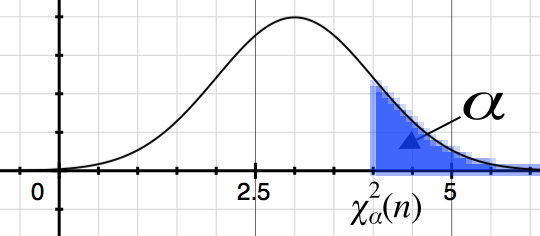
\includegraphics[scale=0.9]{images/分位点}
			\caption{$\chi^2$分布分位点示例图}
		\end{figure}
		\item $E(\chi^2) = n$,$D(\chi^2)=2n$
		\item 若$\chi_1^2 \sim \chi^2(n_1)$,$\chi_2^2 \sim \chi^2(n_2)$,且$\chi_1^2$与$\chi_2^2$相互独立,则$\chi_1^2 + \chi_2^2 \sim \chi^2(n_1+n_2)$
	\end{enumerate}
\end{enumerate}

\subsubsection{$t$分布}
\begin{enumerate}
	\item $t$分布 \\
	若随机变量$X$与$Y$相互独立,且$X\sim N(0,1)$,$Y\sim \chi^2(n)$,则称随机变量
	\begin{equation}
		T = \frac{X}{\sqrt{\frac{Y}{n}}}
	\end{equation}
	服从自由度为$n$的$t$分布,记做$T \sim t(n)$

	\item $t$分布的性质
	\begin{enumerate}
		\item 满足$X,Y$相互独立,$X\sim N(0,1)$,$Y\sim \chi^2(n)$三个条件的$T = \frac{X}{\sqrt{\frac{Y}{n}}}$称为$t(n)$的典型分布
		\item $t$分布的概率密度$f(x)$是偶函数,即$f(x) = f(-x)$
		\item 当$n$充分大时,$t(n)$分布近似于$N(0,1)$分布
		\item 若$0<\alpha<1$,则称满足条件
		\begin{equation}
			P(T > t_{\alpha}(n)) = \int_{t_{\alpha}(n)}^{+\infty}f(x)dx = \alpha
		\end{equation}
		的点为$t_{\alpha}(n)$为$t(n)$分布的上$\alpha$分位点。
		\item 因为$t(n)$分布的概率密度为偶函数,故可知$t$分布的双侧$\alpha$分位点$t_{\frac{\alpha}{2}}(n)$,即
		\begin{equation}
			P\left(|T|>t_{\frac{\alpha}{2}}(n)\right) = \alpha
		\end{equation}
		\begin{figure}[htbp]
			\centering
			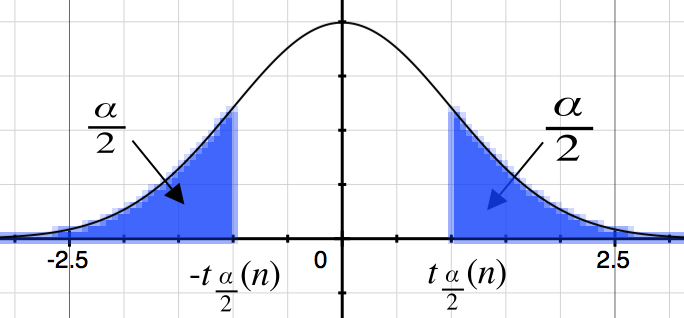
\includegraphics[scale=0.9]{images/t分布分位点}
			\caption{$t$分布分位点示例图}
		\end{figure}
		如图可知,$t_{1-\alpha}(n) = -t_{\alpha}(n)$(将$\frac{\alpha}{2}$用$\alpha$代替,公式更好看)。
	\end{enumerate}
\end{enumerate}

\subsubsection{$F$分布}
\begin{enumerate}
	\item $F$分布 \\
	若随机变量$X$与$Y$相互独立,且$X\sim \chi^2(n_1)$,$Y\sim \chi^2(n_2)$,则称随机变量
	\begin{equation}
		F = \frac{\frac{X}{n_1}}{\frac{Y}{n_2}}
	\end{equation}
	服从自由度为$(n_1, n_2)$的$F$分布,记做$F \sim F(n_1, n_2)$,其中,$n_1, n_2$分别称为第一自由度和第二自由度
	\item $F$分布的性质 \\
	\begin{enumerate}
		\item 满足$X,Y$独立,$X\sim \chi^2(n_1)$,$Y\sim \chi^2(n_2)$三个条件的$F=\frac{\frac{X}{n_1}}{\frac{Y}{n_2}}$称为$F(n_1, n_2)$的典型模式
		\item 若$0<\alpha<1$,则称满足条件
		\begin{equation}
			P(F > F_{\alpha}(n_1, n_2)) = \int_{F_{\alpha}(n_1, n_2)}^{+\infty}f(x)dx = \alpha
		\end{equation}
		的点为$F_{\alpha}(n_1, n_2)$为$F_{\alpha}(n_1, n_2)$分布的上$\alpha$分位点。
		\item 如果$F\sim F(n_1, n_2)$,则$\frac{1}{F}\sim F(n_2, n_1)$,且有
		\begin{equation}
			F_{1-\alpha}(n_1, n_2) = \frac{1}{F_{\alpha}(n_2, n_1)}
		\end{equation}
	\end{enumerate}
\end{enumerate}


\subsection{正态总体的抽样分布}
\subsubsection{一个正态总体的抽样分布}
设总体$X\sim N(\mu, \sigma^2)$,$X_1, X_2, \dots, X_n$是来自总体的样本,样本均值为$\bar X$,样本方差为$S^2$,则有
\begin{enumerate}
	\item $\bar X \sim N(\mu, \frac{\sigma^2}{n})$, $\frac{\bar X - \mu}{\frac{\sigma}{\sqrt{n}}} \sim N(0,1)$
	\item $\bar X$与$S^2$相互独立,且$\frac{(n-1)S^2}{\sigma^2} \sim \chi^2(n-1)$
	\item $\frac{\bar X - \mu}{\frac{S}{\sqrt{n}}} \sim t(n-1)$
	\item $\frac{1}{\sigma^2}\sum_{i=1}^{n}(X_i-\mu)^2 \sim \chi^2(n)$
\end{enumerate}

\subsubsection{两个正态总体的抽样分布}
设总体$X\sim N(\mu_1, \sigma_1^2)$和总体$Y \sim N(\mu_2, \sigma_2^2)$,$X_1, X_2, \dots, X_{n_1}$,$Y_1, Y_2, \dots, Y_{n_2}$是分别来自总体$X$和总体$Y$的样本,且相互独立,样本均值分别为$\bar X$和$\bar Y$,样本方差分别为$S_1^2$和$S_2^2$,则有
\begin{enumerate}
	\item $\bar X - \bar Y \sim N(\mu_1-\mu_2, \frac{\sigma_1^2}{n_1}+\frac{\sigma_2^2}{n_2})$, $\frac{(\bar X - \bar Y)-(\mu_1-\mu_2)}{\sqrt{\frac{\sigma_1^2}{n_1}+\frac{\sigma_2^2}{n_2}}} \sim N(0,1)$
	\item 若$\sigma_1^2 = \sigma_2^2$,则
	\begin{equation}
		\frac{\bar X - \bar Y-(\mu_1 - \mu_2)}{S_\omega \sqrt{\frac{1}{n_1} + \frac{1}{n_2}}} \sim t(n_1+n_2-2)
	\end{equation}
	其中,$S_\omega^2 = \frac{(n_1-1)S_1^2+ (n_2-1)S_2^2}{n_1+n_2-2}$
	\item 
	\begin{equation}
		\frac{\frac{S_1^2}{\sigma_1^2}}{\frac{S_2^2}{\sigma_2^2}} \sim F(n_1-1, n_2-1)
	\end{equation}
\end{enumerate}





















		\section{参数估计}
\subsection{点估计}
\begin{enumerate}
	\item 点估计 
	\footnote{为了区分估计量与实际值,我们给估计量带个帽子,如:$\hat{\theta}$} \\
	用样本$X_1, X_2, \dots, X_n$构造的统计量$\hat{\theta}(X_1, X_2, \dots, X_n)$来估计未知参数$\theta$称为点估计,统计量$\hat{\theta}(X_1, X_2, \dots, X_n)$称为估计量
	\item 无偏估计量 \\
	若$\hat{\theta}$是$\theta$的估计量,如果$E(\hat{\theta})=\theta$,则称$\hat{\theta} = \hat{\theta}(X_1, X_2, \dots, X_n)$是未知参数$\theta$的无偏估计量
	\item 更有效估计量 \\
	若$\hat{\theta_1}$和$\hat{\theta_2}$都是$\theta$的无偏估计量,且$D(\hat{\theta_1})\leq D(\hat{\theta_2})$,则称$\hat{\theta_1}$比$\hat{\theta_2}$更有效,或$\hat{\theta_1}$比$\hat{\theta_2}$更有效估计量
	\item 一致估计量 \\
	若$\hat{\theta}(X_1, X_2, \dots, X_n)$是$\theta$的估计值,如果$\hat{\theta}$依概率收敛于$\theta$,则称$\hat{\theta}(X_1, X_2, \dots, X_n)$为$\theta$的一致估计量
	\item 估计量\&统计量 \\
	估计量来自于样本,是一个值;\\
	统计量同样来自样本,但它是一个关于样本的,不含未知参数的函数。
\end{enumerate}

\subsection{矩估计法}
\begin{enumerate}
	\item 矩估计法 \\
	用样本矩估计相应的总体矩,用样本矩的函数估计总体矩相应的函数,然后求出要估计的参数,称这种估计法为矩估计法
	\item 矩估计法的步骤 \\
	略
\end{enumerate}

\subsection{最大似然估计法}
\begin{enumerate}
	\item 似然函数
	\begin{enumerate}
		\item 离散型 \\
		假设其概率分布为:$P(X=a_i) = p(a_i;\theta), \quad i=1,2, \dots$,则似然函数为
		\begin{equation}
			L(\theta) = L(X_1, X_2, \dots, X_n; \theta) = \prod_{i=1}^{n}p(X_i;\theta)
		\end{equation}
		\item 连续型 \\
		假设其概率密度为$f(x;\theta)$,则其似然函数为:
		\begin{equation}
			L(\theta) = L(X_1, X_2, \dots, X_n; \theta) = \prod_{i=1}^{n}f(X_i;\theta)
		\end{equation}
	\end{enumerate}
	\item 最大似然估计法求解步骤
	\begin{enumerate}
		\item 写出似然函数
		\item 求似然函数的导数
		\begin{equation}
			\frac{\mathrm{d}L(\theta)}{\mathrm{d}\theta} = 0
		\end{equation}
		或其对数的导数
		\begin{equation}
			\frac{\mathrm{d}\ln L(\theta)}{\mathrm{d}\theta} = 0
		\end{equation}
		\item 解方程组,得到其驻点
		\item 对每个驻点进行分析,得到最值
		\item 注意:有时使得似然函数达到最值的$\hat{\theta}$不一定是$L(\theta)$或$\ln L(\theta)$的驻点,这种情况下不能用似然方法来求解,应使用其他方法
	\end{enumerate}
\end{enumerate}

\subsection{区间估计}
\begin{enumerate}
	\item 置信区间 \\
	设$\theta$是总体$X$的未知参数,$X_1, X_2, \dots, X_n$是来自总体$X$的样本,对于给定的$\alpha(0<\alpha<1)$,如果两个统计量满足
	\begin{equation}
		P(\theta_1<\theta<\theta_2) = 1-\alpha
	\end{equation}
	则称随机区间$(\theta_1, \theta_2)$为参数$\theta$的置信水平(或置信度)为$1-\alpha$的置信区间(或区间估计),简称为$\theta$的$1-\alpha$置信区间,$\theta_1$和$\theta_2$分别称为置信下限和置信上限
	\item 一个正态总体参数的区间估计 \\
	略
	\item 两个正态总体参数的区间估计 \\
	略
\end{enumerate}
















		\section{假设检验}
\subsection{假设检验}
\begin{enumerate}
	\item 实际推断原理: 小概率事件在一次试验中是不会发生的。 \\
	实际推断原理又称小概率原理。
	\item 假设检验
	\begin{enumerate}
		\item 假设是关于总体的论断或命题,常用字母"$H$"表示。
		\item 假设分为基本假设$H_0$和备选假设 \\
		基本假设又称原假设、零假设 \\
		备选假设又称备择假设、对立假设
		\item 假设检验: 根据样本,按照一定规则判断所做假设$H_0$的真伪,并作出接受还是拒绝接受$H_0$的决定。
	\end{enumerate}
	\item 两类错误
	\begin{enumerate}
		\item 拒绝实际真的假设$H_0$(弃真)称为第一类错误
		\item 接受实际不真的假设$H_0$(纳伪)称为第二类错误
	\end{enumerate}
	\item 显著性检验
	\begin{enumerate}
		\item 显著性水平:在假设检验中允许犯第一类错误的概率称为显著水平,记为$\alpha(0<\alpha<1)$。
		它表现了对$H_0$弃真的控制程度,一般$\alpha$取0.1, 0.05, 0.01, 0.001等
		\item 显著性检验: 只控制第一类错误概率$\alpha$的统计检验称为显著性检验
		\item 显著性检验的一般步骤 \\
		略
	\end{enumerate}
\end{enumerate}


\subsection{正态总体参数的假设检验}
略











		\section{中心极限定理}
\subsection{待添加}
		\section{常用公式}
\begin{enumerate}
	\item 
	\begin{equation}
		\sum_{k=0}^{+\infty}\frac{x^k}{k!} \approx e^x
	\end{equation}

	\item 变上下积分求导公式
	\begin{equation}
		\frac{d}{dy}\int_{\alpha{(y)}}^{\beta{(y)}}f(x)dx = f(\beta(y)){\beta^{'}(y)} - f(\alpha(y)){\alpha^{'}(y)}
	\end{equation}

	\item 等比数列求和公式
	\begin{equation}
	 	\begin{aligned}
			S_n &= n a_1 \quad (q = 1) \\
			S_n &=  \frac{a_1(1-q^n)}{1-q} = \frac{a_1 - a_n q}{1-q} \quad (q \neq 1)
		\end{aligned}
	 \end{equation}

	 \item 最大最小值公式
	 \begin{align}
	 	\max(X,Y) &= \frac{X+Y+|X-Y|}{2} \\
	 	\min(X,Y) &= \frac{X+Y-|X-Y|}{2}
	 \end{align}


\end{enumerate}


\end{document}










